\section{Supplementary results}
\label{sec:result_balibase}

% Table generated by Excel2LaTeX from sheet 'pasta varaints (2)'
\begin{table}[htbp]
	\centering
	\small
	\caption{FN rate achieved by the four variants of PASTA for each dataset in set A. On each row, the lower (better) FN rate values are marked with darker color.}
	\begin{tabular}{|l|r|r|r|r|}
		\hline
		\multirow{2}{*}{Dataset} & \multicolumn{4}{c|}{FN rate of PASTA variants } \\
		\cline{2-5}          & \multicolumn{1}{l|}{PASTA-3I-D} & \multicolumn{1}{l|}{PASTA-8I-D} & \multicolumn{1}{l|}{PASTA-3I-S} & \multicolumn{1}{l|}{PASTA-8I-S} \\
		\hline
		BB11005 & \cellcolor[rgb]{ .384,  .745,  .478}0.27 & \cellcolor[rgb]{ .988,  1,  .992}0.55 & \cellcolor[rgb]{ .584,  .827,  .647}0.36 & \cellcolor[rgb]{ .384,  .745,  .478}0.27 \\
		\hline
		BB11018 & \cellcolor[rgb]{ .384,  .745,  .478}0.27 & \cellcolor[rgb]{ .384,  .745,  .478}0.27 & \cellcolor[rgb]{ .584,  .827,  .647}0.36 & \cellcolor[rgb]{ .988,  1,  .992}0.55 \\
		\hline
		BB11020 & \cellcolor[rgb]{ .686,  .871,  .733}0.67 & \cellcolor[rgb]{ .988,  1,  .992}0.83 & \cellcolor[rgb]{ .384,  .745,  .478}0.50 & \cellcolor[rgb]{ .384,  .745,  .478}0.50 \\
		\hline
		BB11033 & \cellcolor[rgb]{ .502,  .796,  .58}0.50 & \cellcolor[rgb]{ .384,  .745,  .478}0.38 & \cellcolor[rgb]{ .624,  .847,  .682}0.63 & \cellcolor[rgb]{ .988,  1,  .992}1.00 \\
		\hline
		BB12001 & \cellcolor[rgb]{ .988,  1,  .992}0.50 & \cellcolor[rgb]{ .384,  .745,  .478}0.25 & \cellcolor[rgb]{ .686,  .871,  .733}0.38 & \cellcolor[rgb]{ .686,  .871,  .733}0.38 \\
		\hline
		BB12013 & \cellcolor[rgb]{ .988,  1,  .992}0.20 & \cellcolor[rgb]{ .988,  1,  .992}0.20 & \cellcolor[rgb]{ .988,  1,  .992}0.20 & \cellcolor[rgb]{ .988,  1,  .992}0.20 \\
		\hline
		BB12022 & \cellcolor[rgb]{ .384,  .745,  .478}0.00 & \cellcolor[rgb]{ .384,  .745,  .478}0.00 & \cellcolor[rgb]{ .384,  .745,  .478}0.00 & \cellcolor[rgb]{ .988,  1,  .992}0.50 \\
		\hline
		BB12035 & \cellcolor[rgb]{ .467,  .78,  .549}0.04 & \cellcolor[rgb]{ .384,  .745,  .478}0.00 & \cellcolor[rgb]{ .467,  .78,  .549}0.04 & \cellcolor[rgb]{ .988,  1,  .992}0.29 \\
		\hline
		BB12044 & \cellcolor[rgb]{ .988,  1,  .992}0.50 & \cellcolor[rgb]{ .988,  1,  .992}0.50 & \cellcolor[rgb]{ .384,  .745,  .478}0.38 & \cellcolor[rgb]{ .384,  .745,  .478}0.38 \\
		\hline
		BB20002 & \cellcolor[rgb]{ .988,  1,  .992}0.65 & \cellcolor[rgb]{ .988,  1,  .992}0.65 & \cellcolor[rgb]{ .988,  1,  .992}0.65 & \cellcolor[rgb]{ .988,  1,  .992}0.65 \\
		\hline
		BB20010 & \cellcolor[rgb]{ .988,  1,  .992}0.38 & \cellcolor[rgb]{ .835,  .933,  .863}0.35 & \cellcolor[rgb]{ .686,  .871,  .733}0.31 & \cellcolor[rgb]{ .384,  .745,  .478}0.23 \\
		\hline
		BB20022 & \cellcolor[rgb]{ .988,  1,  .992}0.11 & \cellcolor[rgb]{ .988,  1,  .992}0.11 & \cellcolor[rgb]{ .988,  1,  .992}0.11 & \cellcolor[rgb]{ .988,  1,  .992}0.11 \\
		\hline
		BB20033 & \cellcolor[rgb]{ .988,  1,  .992}0.38 & \cellcolor[rgb]{ .835,  .933,  .863}0.36 & \cellcolor[rgb]{ .988,  1,  .992}0.38 & \cellcolor[rgb]{ .384,  .745,  .478}0.29 \\
		\hline
		BB20041 & \cellcolor[rgb]{ .502,  .792,  .58}0.40 & \cellcolor[rgb]{ .384,  .745,  .478}0.38 & \cellcolor[rgb]{ .624,  .843,  .682}0.42 & \cellcolor[rgb]{ .988,  1,  .992}0.49 \\
		\hline
		BB30002 & \cellcolor[rgb]{ .988,  1,  .992}0.32 & \cellcolor[rgb]{ .988,  1,  .992}0.32 & \cellcolor[rgb]{ .988,  1,  .992}0.32 & \cellcolor[rgb]{ .988,  1,  .992}0.32 \\
		\hline
		BB30008 & \cellcolor[rgb]{ .384,  .745,  .478}0.33 & \cellcolor[rgb]{ .384,  .745,  .478}0.33 & \cellcolor[rgb]{ .584,  .827,  .647}0.36 & \cellcolor[rgb]{ .988,  1,  .992}0.42 \\
		\hline
		BB30015 & \cellcolor[rgb]{ .384,  .745,  .478}0.17 & \cellcolor[rgb]{ .384,  .745,  .478}0.17 & \cellcolor[rgb]{ .384,  .745,  .478}0.17 & \cellcolor[rgb]{ .988,  1,  .992}0.33 \\
		\hline
		BB30022 & \cellcolor[rgb]{ .988,  1,  .992}0.54 & \cellcolor[rgb]{ .584,  .827,  .647}0.51 & \cellcolor[rgb]{ .384,  .745,  .478}0.49 & \cellcolor[rgb]{ .584,  .827,  .647}0.51 \\
		\hline
		BB40001 & \cellcolor[rgb]{ .988,  1,  .992}0.68 & \cellcolor[rgb]{ .384,  .745,  .478}0.48 & \cellcolor[rgb]{ .624,  .847,  .682}0.56 & \cellcolor[rgb]{ .384,  .745,  .478}0.48 \\
		\hline
		BB40013 & \cellcolor[rgb]{ .384,  .745,  .478}0.38 & \cellcolor[rgb]{ .384,  .745,  .478}0.38 & \cellcolor[rgb]{ .384,  .745,  .478}0.38 & \cellcolor[rgb]{ .988,  1,  .992}0.47 \\
		\hline
		BB40025 & \cellcolor[rgb]{ .384,  .745,  .478}0.00 & \cellcolor[rgb]{ .384,  .745,  .478}0.00 & \cellcolor[rgb]{ .384,  .745,  .478}0.00 & \cellcolor[rgb]{ .988,  1,  .992}0.09 \\
		\hline
		BB40038 & \cellcolor[rgb]{ .988,  1,  .992}0.25 & \cellcolor[rgb]{ .988,  1,  .992}0.25 & \cellcolor[rgb]{ .988,  1,  .992}0.25 & \cellcolor[rgb]{ .988,  1,  .992}0.25 \\
		\hline
		BB40048 & \cellcolor[rgb]{ .384,  .745,  .478}0.29 & \cellcolor[rgb]{ .988,  1,  .992}0.43 & \cellcolor[rgb]{ .384,  .745,  .478}0.29 & \cellcolor[rgb]{ .384,  .745,  .478}0.29 \\
		\hline
		BB50001 & \cellcolor[rgb]{ .988,  1,  .992}0.32 & \cellcolor[rgb]{ .384,  .745,  .478}0.29 & \cellcolor[rgb]{ .988,  1,  .992}0.32 & \cellcolor[rgb]{ .384,  .745,  .478}0.29 \\
		\hline
		BB50005 & \cellcolor[rgb]{ .988,  1,  .992}0.38 & \cellcolor[rgb]{ .988,  1,  .992}0.38 & \cellcolor[rgb]{ .988,  1,  .992}0.38 & \cellcolor[rgb]{ .988,  1,  .992}0.38 \\
		\hline
		BB50010 & \cellcolor[rgb]{ .988,  1,  .992}0.07 & \cellcolor[rgb]{ .384,  .745,  .478}0.00 & \cellcolor[rgb]{ .988,  1,  .992}0.07 & \cellcolor[rgb]{ .384,  .745,  .478}0.00 \\
		\hline
		BB50016 & \cellcolor[rgb]{ .384,  .745,  .478}0.27 & \cellcolor[rgb]{ .988,  1,  .992}0.47 & \cellcolor[rgb]{ .384,  .745,  .478}0.27 & \cellcolor[rgb]{ .384,  .745,  .478}0.27 \\
		\hline		
	\end{tabular}%
	\label{tab:pasta-variants-a}%
\end{table}%



\begin{table}[htbp]
	\centering
	\small
	\caption{FN rate achieved by the four variants of PASTA for each dataset in set B. On each row, the lower (better) FN rate values are marked with darker color.}
	\begin{tabular}{|l|r|r|r|r|}
		\hline
		\multirow{2}{*}{Dataset} & \multicolumn{4}{c|}{FN rate of PASTA variants} \\
		\cline{2-5}          & \multicolumn{1}{l|}{PASTA-3I-D} & \multicolumn{1}{l|}{PASTA-8I-D} & \multicolumn{1}{l|}{PASTA-3I-S} & \multicolumn{1}{l|}{PASTA-8I-S} \\
		\hline
		BB11007 & \cellcolor[rgb]{ .988,  1,  .992}0.67 & \cellcolor[rgb]{ .384,  .745,  .478}0.50 & \cellcolor[rgb]{ .988,  1,  .992}0.67 & \cellcolor[rgb]{ .384,  .745,  .478}0.50 \\
		\hline
		BB11019 & \cellcolor[rgb]{ .988,  1,  .992}0.43 & \cellcolor[rgb]{ .682,  .871,  .733}0.29 & \cellcolor[rgb]{ .384,  .745,  .478}0.14 & \cellcolor[rgb]{ .682,  .871,  .733}0.29 \\
		\hline
		BB11034 & \cellcolor[rgb]{ .384,  .745,  .478}0.20 & \cellcolor[rgb]{ .686,  .871,  .733}0.40 & \cellcolor[rgb]{ .686,  .871,  .733}0.40 & \cellcolor[rgb]{ .988,  1,  .992}0.60 \\
		\hline
		BB11038 & \cellcolor[rgb]{ .384,  .745,  .478}0.40 & \cellcolor[rgb]{ .384,  .745,  .478}0.40 & \cellcolor[rgb]{ .988,  1,  .992}0.60 & \cellcolor[rgb]{ .988,  1,  .992}0.60 \\
		\hline
		BB12005 & \cellcolor[rgb]{ .384,  .745,  .478}0.33 & \cellcolor[rgb]{ .384,  .745,  .478}0.33 & \cellcolor[rgb]{ .384,  .745,  .478}0.33 & \cellcolor[rgb]{ .988,  1,  .992}0.50 \\
		\hline
		BB12026 & \cellcolor[rgb]{ .384,  .745,  .478}0.40 & \cellcolor[rgb]{ .624,  .843,  .682}0.53 & \cellcolor[rgb]{ .624,  .843,  .682}0.53 & \cellcolor[rgb]{ .988,  1,  .992}0.73 \\
		\hline
		BB12029 & \cellcolor[rgb]{ .988,  1,  .992}0.44 & \cellcolor[rgb]{ .988,  1,  .992}0.44 & \cellcolor[rgb]{ .988,  1,  .992}0.44 & \cellcolor[rgb]{ .988,  1,  .992}0.44 \\
		\hline
		BB12037 & \cellcolor[rgb]{ .482,  .784,  .561}0.30 & \cellcolor[rgb]{ .584,  .827,  .647}0.40 & \cellcolor[rgb]{ .988,  1,  .992}0.80 & \cellcolor[rgb]{ .384,  .745,  .478}0.20 \\
		\hline
		BB20002 & \cellcolor[rgb]{ .988,  1,  .992}0.65 & \cellcolor[rgb]{ .988,  1,  .992}0.65 & \cellcolor[rgb]{ .988,  1,  .992}0.65 & \cellcolor[rgb]{ .988,  1,  .992}0.65 \\
		\hline
		BB20012 & \cellcolor[rgb]{ .686,  .871,  .733}0.29 & \cellcolor[rgb]{ .686,  .871,  .733}0.29 & \cellcolor[rgb]{ .988,  1,  .992}0.33 & \cellcolor[rgb]{ .384,  .745,  .478}0.25 \\
		\hline
		BB20030 & \cellcolor[rgb]{ .384,  .745,  .478}0.64 & \cellcolor[rgb]{ .384,  .745,  .478}0.64 & \cellcolor[rgb]{ .502,  .792,  .58}0.66 & \cellcolor[rgb]{ .988,  1,  .992}0.75 \\
		\hline
		BB20037 & \cellcolor[rgb]{ .988,  1,  .992}0.29 & \cellcolor[rgb]{ .384,  .745,  .478}0.13 & \cellcolor[rgb]{ .867,  .949,  .886}0.26 & \cellcolor[rgb]{ .804,  .922,  .835}0.24 \\
		\hline
		BB30003 & \cellcolor[rgb]{ .682,  .871,  .733}0.30 & \cellcolor[rgb]{ .682,  .871,  .733}0.30 & \cellcolor[rgb]{ .988,  1,  .992}0.31 & \cellcolor[rgb]{ .384,  .745,  .478}0.29 \\
		\hline
		BB30011 & \cellcolor[rgb]{ .988,  1,  .992}0.35 & \cellcolor[rgb]{ .988,  1,  .992}0.35 & \cellcolor[rgb]{ .988,  1,  .992}0.35 & \cellcolor[rgb]{ .988,  1,  .992}0.35 \\
		\hline
		BB30021 & \cellcolor[rgb]{ .522,  .804,  .596}0.38 & \cellcolor[rgb]{ .451,  .773,  .537}0.36 & \cellcolor[rgb]{ .988,  1,  .992}0.53 & \cellcolor[rgb]{ .384,  .745,  .478}0.34 \\
		\hline
		BB30026 & \cellcolor[rgb]{ .988,  1,  .992}0.22 & \cellcolor[rgb]{ .384,  .745,  .478}0.19 & \cellcolor[rgb]{ .988,  1,  .992}0.22 & \cellcolor[rgb]{ .682,  .871,  .733}0.21 \\
		\hline
		BB40006 & \cellcolor[rgb]{ .988,  1,  .992}0.00 & \cellcolor[rgb]{ .988,  1,  .992}0.00 & \cellcolor[rgb]{ .988,  1,  .992}0.00 & \cellcolor[rgb]{ .988,  1,  .992}0.00 \\
		\hline
		BB40009 & \cellcolor[rgb]{ .988,  1,  .992}0.19 & \cellcolor[rgb]{ .988,  1,  .992}0.19 & \cellcolor[rgb]{ .988,  1,  .992}0.19 & \cellcolor[rgb]{ .988,  1,  .992}0.19 \\
		\hline
		BB40019 & \cellcolor[rgb]{ .988,  1,  .992}0.43 & \cellcolor[rgb]{ .988,  1,  .992}0.43 & \cellcolor[rgb]{ .988,  1,  .992}0.43 & \cellcolor[rgb]{ .988,  1,  .992}0.43 \\
		\hline
		BB40033 & \cellcolor[rgb]{ .384,  .745,  .478}0.06 & \cellcolor[rgb]{ .988,  1,  .992}0.13 & \cellcolor[rgb]{ .988,  1,  .992}0.13 & \cellcolor[rgb]{ .988,  1,  .992}0.13 \\
		\hline
		BB50002 & \cellcolor[rgb]{ .988,  1,  .992}0.60 & \cellcolor[rgb]{ .384,  .745,  .478}0.50 & \cellcolor[rgb]{ .988,  1,  .992}0.60 & \cellcolor[rgb]{ .384,  .745,  .478}0.50 \\
		\hline
		BB50006 & \cellcolor[rgb]{ .384,  .745,  .478}0.21 & \cellcolor[rgb]{ .384,  .745,  .478}0.21 & \cellcolor[rgb]{ .835,  .933,  .863}0.26 & \cellcolor[rgb]{ .988,  1,  .992}0.28 \\
		\hline
		BB50009 & \cellcolor[rgb]{ .384,  .745,  .478}0.16 & \cellcolor[rgb]{ .784,  .914,  .82}0.24 & \cellcolor[rgb]{ .584,  .827,  .647}0.20 & \cellcolor[rgb]{ .988,  1,  .992}0.28 \\
		\hline
		BB50014 & \cellcolor[rgb]{ .988,  1,  .992}0.44 & \cellcolor[rgb]{ .384,  .745,  .478}0.41 & \cellcolor[rgb]{ .988,  1,  .992}0.44 & \cellcolor[rgb]{ .988,  1,  .992}0.44 \\
		\hline
	\end{tabular}%
	\label{tab:pasta-variants-b}%
\end{table}%

% Table generated by Excel2LaTeX from sheet 'stat test'
\begin{table}[htbp]
	\small
	\centering
	\caption{\underline{Friedman Aligned Ranks test (Column 2):} Friedman Aligned ranks (lower is better) of the four variants of PASTA based on Table~\ref{tab:pasta-variants-a}, \ref{tab:pasta-variants-b}. We also show the computed statistics and corresponding $ p $-value. 
		\underline{Holm's post-hoc procedure (Columns 3 - 6):} Comparison among the PASTA variants using the Holm's post-hoc procedures. Each entry shows the adjusted $p$-value which indicates the significance of the difference in performance between two methods.}
	\begin{tabular}{|l|r||c|c|c|c|}
		\hline
		\multicolumn{1}{|c|}{1} & \multicolumn{1}{c||}{2} & \multicolumn{1}{c|}{3} & \multicolumn{1}{c|}{4} & \multicolumn{1}{c|}{5} & 6 \\
		\hline
		\multirow{2}{*}{\makecell{PASTA\\ variants}} & \multirow{2}{*}{\makecell{Friedman Aligned\\ rank*}} & \multicolumn{4}{c|}{Holm's adjusted $p$-value} \\
		\cline{3-6}          &       & 8I-D & 3I-D & 3I-S & 8I-S \\
		\hline
		8I-D  & 89.2843 & \multicolumn{1}{c|}{-} & \multicolumn{1}{r|}{1.0000} & \multicolumn{1}{r|}{0.4481} & \multicolumn{1}{r|}{0.1746} \\
		\hline
		3I-D  & 96.7941 & \multicolumn{1}{r|}{1.0000} & \multicolumn{1}{c|}{-} & \multicolumn{1}{r|}{0.8743} & \multicolumn{1}{r|}{0.4945} \\
		\hline
		3I-S  & 109.1275 & \multicolumn{1}{r|}{0.4481} & \multicolumn{1}{r|}{0.8743} & \multicolumn{1}{c|}{-} & \multicolumn{1}{r|}{1.0000} \\
		\hline
		8I-S  & 114.7941 & \multicolumn{1}{r|}{0.1746} & \multicolumn{1}{r|}{0.4945} & \multicolumn{1}{r|}{1.0000} & - \\
		\hline
		*Statistic & 4.8016 & \multicolumn{4}{c|}{\multirow{2}{*}{N/A}} \\
		\cline{1-2}    *$p$-value & 0.1869 & \multicolumn{4}{c|}{} \\
		\hline
	\end{tabular}%
	\label{tab:test-pasta-variants}%
\end{table}%

\begin{figure}[!htbp]%
	\begin{adjustwidth}{-1.0cm}{}
	\centering
	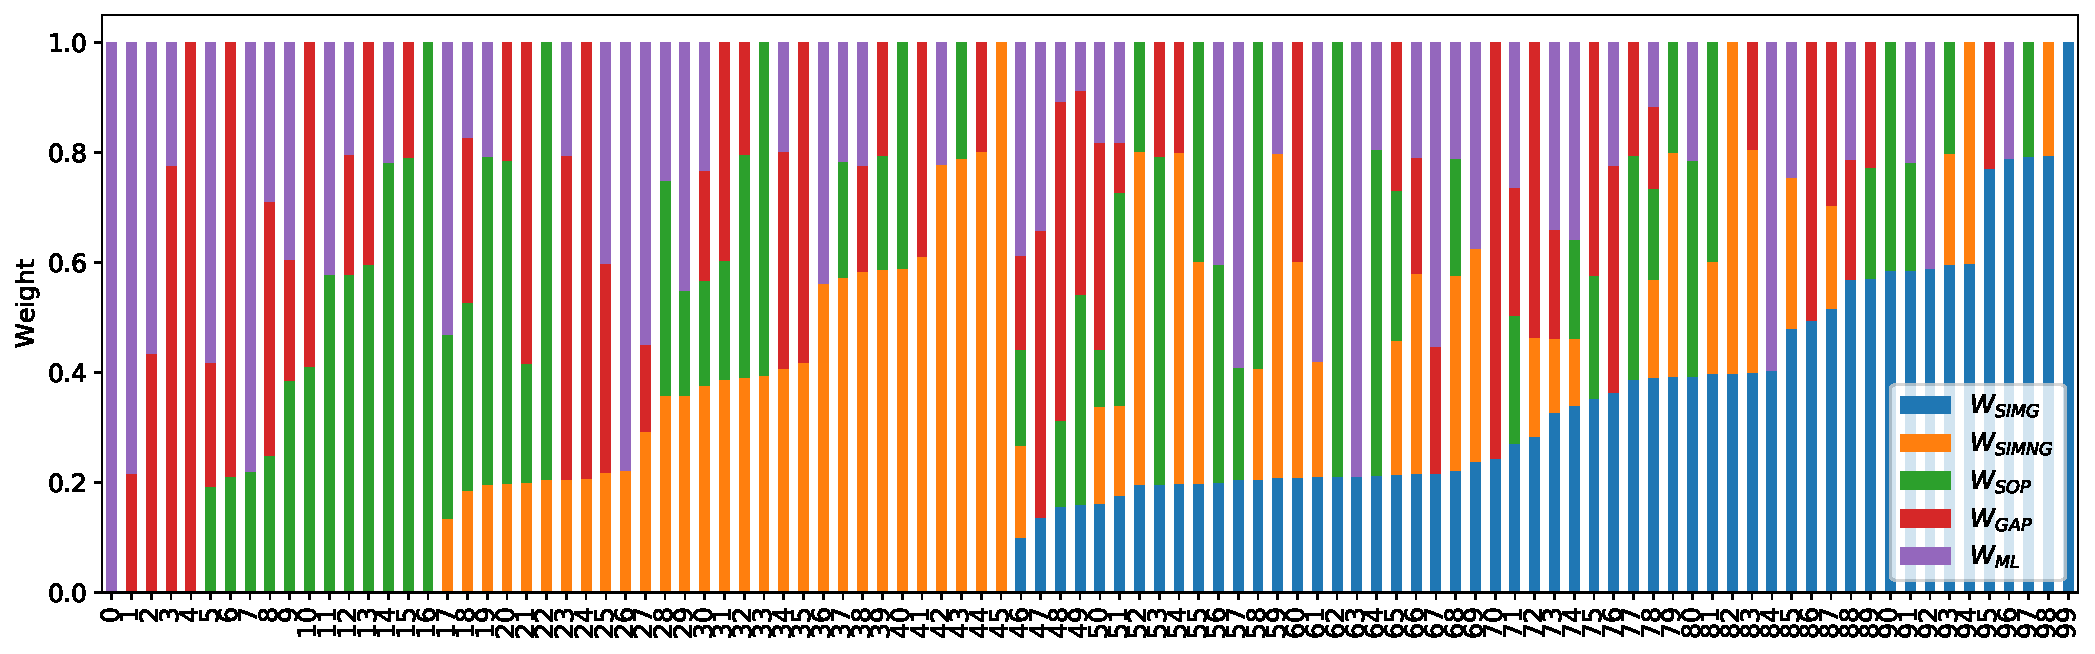
\includegraphics[width=\textwidth]{100-weights}
	\caption{100 well-spaced 5D weight vectors. Each vertical bar depicts one weight vector.}
	\label{fig:100-weights}
		\end{adjustwidth}
\end{figure}

% Table generated by Excel2LaTeX from sheet 'stat-8I-30w-S'
\begin{table}[htbp]
	\scriptsize
	\centering
	\caption{Comparison of the 100 solutions generated by PMAO using 100 input vectors with respect to PASTA's FN rate on set A datasets. For PMAO, we show the best FN rate along with the average FN rate 
		and count of its solutions better or equivalent to PASTA. The better values are marked with darker shade.}
	\begin{tabular}{|l|r|r|r||r|}
		\hline
		\multirow{2}{*}{Dataset} & \multirow{2}{*}{\makecell{PASTA\\FN rate}} & \multicolumn{3}{c|}{\makecell{PMAO solutions better \\or equivalent to PASTA}} \\
		\cline{3-5}          &       & \multicolumn{1}{l|}{Best FN} & \multicolumn{1}{l||}{Avg FN} & \multicolumn{1}{l|}{Count} \\
		\hline
		BB11005 & \cellcolor[rgb]{ .988,  1,  .992}0.55 & \cellcolor[rgb]{ .384,  .745,  .478}0.09 & \cellcolor[rgb]{ .71,  .882,  .757}0.34 & \cellcolor[rgb]{ .976,  .455,  .463}93 \\
		\hline
		BB11018 & \cellcolor[rgb]{ .988,  1,  .992}0.27 & \cellcolor[rgb]{ .384,  .745,  .478}0.18 & \cellcolor[rgb]{ .843,  .937,  .867}0.25 & \cellcolor[rgb]{ .988,  .855,  .867}25 \\
		\hline
		BB11033 & \cellcolor[rgb]{ .988,  1,  .992}0.38 & \cellcolor[rgb]{ .384,  .745,  .478}0.25 & \cellcolor[rgb]{ .957,  .984,  .965}0.37 & \cellcolor[rgb]{ .988,  .882,  .894}20 \\
		\hline
		BB11020 & \cellcolor[rgb]{ .988,  1,  .992}0.83 & \cellcolor[rgb]{ .384,  .745,  .478}0.17 & \cellcolor[rgb]{ .773,  .91,  .808}0.60 & \cellcolor[rgb]{ .973,  .412,  .42}100 \\
		\hline
		BB12001 & \cellcolor[rgb]{ .988,  1,  .992}0.25 & \cellcolor[rgb]{ .384,  .745,  .478}0.13 & \cellcolor[rgb]{ .933,  .976,  .945}0.24 & \cellcolor[rgb]{ .98,  .667,  .675}57 \\
		\hline
		BB12013 & \cellcolor[rgb]{ .988,  1,  .992}0.20 & \cellcolor[rgb]{ .384,  .745,  .478}0.00 & \cellcolor[rgb]{ .949,  .984,  .961}0.19 & \cellcolor[rgb]{ .976,  .42,  .427}99 \\
		\hline
		BB12022 & \cellcolor[rgb]{ .988,  1,  .992}0.00 & \cellcolor[rgb]{ .988,  1,  .992}0.00 & \cellcolor[rgb]{ .988,  1,  .992}0.00 & \cellcolor[rgb]{ .976,  .482,  .494}88 \\
		\hline
		BB12035 & \cellcolor[rgb]{ .988,  1,  .992}0.00 & \cellcolor[rgb]{ .988,  1,  .992}0.00 & \cellcolor[rgb]{ .988,  1,  .992}0.00 & \cellcolor[rgb]{ .988,  .988,  1}2 \\
		\hline
		BB12044 & \cellcolor[rgb]{ .988,  1,  .992}0.50 & \cellcolor[rgb]{ .384,  .745,  .478}0.25 & \cellcolor[rgb]{ .847,  .941,  .871}0.44 & \cellcolor[rgb]{ .973,  .412,  .42}100 \\
		\hline
		BB20001 & \cellcolor[rgb]{ .988,  1,  .992}0.54 & \cellcolor[rgb]{ .384,  .745,  .478}0.08 & \cellcolor[rgb]{ .886,  .957,  .906}0.46 & \cellcolor[rgb]{ .98,  .596,  .604}69 \\
		\hline
		BB20010 & \cellcolor[rgb]{ .988,  1,  .992}0.35 & \cellcolor[rgb]{ .384,  .745,  .478}0.08 & \cellcolor[rgb]{ .863,  .945,  .886}0.29 & \cellcolor[rgb]{ .976,  .502,  .51}85 \\
		\hline
		BB20022 & \cellcolor[rgb]{ .988,  1,  .992}0.11 & \cellcolor[rgb]{ .384,  .745,  .478}0.09 & \cellcolor[rgb]{ .969,  .992,  .976}0.11 & \cellcolor[rgb]{ .984,  .804,  .812}34 \\
		\hline
		BB20033 & \cellcolor[rgb]{ .988,  1,  .992}0.36 & \cellcolor[rgb]{ .384,  .745,  .478}0.27 & \cellcolor[rgb]{ .737,  .894,  .78}0.32 & \cellcolor[rgb]{ .984,  .82,  .831}31 \\
		\hline
		BB20041 & \cellcolor[rgb]{ .988,  1,  .992}0.38 & \cellcolor[rgb]{ .384,  .745,  .478}0.31 & \cellcolor[rgb]{ .839,  .937,  .867}0.36 & \cellcolor[rgb]{ .988,  .847,  .859}26 \\
		\hline
		BB30002 & \cellcolor[rgb]{ .988,  1,  .992}0.32 & \cellcolor[rgb]{ .384,  .745,  .478}0.14 & \cellcolor[rgb]{ .902,  .961,  .918}0.30 & \cellcolor[rgb]{ .98,  .694,  .706}52 \\
		\hline
		BB30008 & \cellcolor[rgb]{ .988,  1,  .992}0.33 & \cellcolor[rgb]{ .384,  .745,  .478}0.21 & \cellcolor[rgb]{ .859,  .945,  .882}0.31 & \cellcolor[rgb]{ .984,  .753,  .765}42 \\
		\hline
		BB30015 & \cellcolor[rgb]{ .988,  1,  .992}0.17 & \cellcolor[rgb]{ .384,  .745,  .478}0.11 & \cellcolor[rgb]{ .969,  .992,  .976}0.17 & \cellcolor[rgb]{ .984,  .788,  .8}36 \\
		\hline
		BB30022 & \cellcolor[rgb]{ .988,  1,  .992}0.51 & \cellcolor[rgb]{ .384,  .745,  .478}0.44 & \cellcolor[rgb]{ .91,  .965,  .925}0.50 & \cellcolor[rgb]{ .98,  .675,  .682}56 \\
		\hline
		BB40001 & \cellcolor[rgb]{ .988,  1,  .992}0.48 & \cellcolor[rgb]{ .384,  .745,  .478}0.32 & \cellcolor[rgb]{ .776,  .91,  .812}0.42 & \cellcolor[rgb]{ .988,  .878,  .89}21 \\
		\hline
		BB40013 & \cellcolor[rgb]{ .988,  1,  .992}0.38 & \cellcolor[rgb]{ .384,  .745,  .478}0.28 & \cellcolor[rgb]{ .765,  .906,  .8}0.34 & \cellcolor[rgb]{ .98,  .667,  .675}57 \\
		\hline
		BB40025 & \cellcolor[rgb]{ .988,  1,  .992}0.00 & \cellcolor[rgb]{ .988,  1,  .992}0.00 & \cellcolor[rgb]{ .988,  1,  .992}0.00 & \cellcolor[rgb]{ .98,  .643,  .651}61 \\
		\hline
		BB40038 & \cellcolor[rgb]{ .988,  1,  .992}0.25 & \cellcolor[rgb]{ .384,  .745,  .478}0.10 & \cellcolor[rgb]{ .769,  .906,  .808}0.20 & \cellcolor[rgb]{ .98,  .616,  .624}66 \\
		\hline
		BB40048 & \cellcolor[rgb]{ .988,  1,  .992}0.43 & \cellcolor[rgb]{ .384,  .745,  .478}0.29 & \cellcolor[rgb]{ .463,  .776,  .545}0.30 & \cellcolor[rgb]{ .973,  .412,  .42}100 \\
		\hline
		BB50001 & \cellcolor[rgb]{ .988,  1,  .992}0.29 & \cellcolor[rgb]{ .384,  .745,  .478}0.16 & \cellcolor[rgb]{ .902,  .961,  .918}0.27 & \cellcolor[rgb]{ .98,  .62,  .627}65 \\
		\hline
		BB50005 & \cellcolor[rgb]{ .988,  1,  .992}0.38 & \cellcolor[rgb]{ .384,  .745,  .478}0.13 & \cellcolor[rgb]{ .933,  .976,  .945}0.35 & \cellcolor[rgb]{ .973,  .412,  .42}100 \\
		\hline
		BB50010 & \cellcolor[rgb]{ .988,  1,  .992}0.00 & \cellcolor[rgb]{ .988,  1,  .992}0.00 & \cellcolor[rgb]{ .988,  1,  .992}0.00 & \cellcolor[rgb]{ .988,  .937,  .949}11 \\
		\hline
		BB50016 & \cellcolor[rgb]{ .988,  1,  .992}0.47 & \cellcolor[rgb]{ .384,  .745,  .478}0.07 & \cellcolor[rgb]{ .62,  .843,  .678}0.22 & \cellcolor[rgb]{ .976,  .42,  .427}99 \\
		\hline
	\end{tabular}%
	\label{tab:pmao-100}%
\end{table}%


\begin{figure}
	\begin{adjustwidth}{-1.2cm}{-1.2cm}
	\centering
	\def\names{{BB11005},{BB11018},{BB11033},{BB11020},{BB12001},{BB12013},{BB12022},{BB12035},{BB12044},{BB20001},{BB20010},{BB20022},{BB20033},{BB20041},{BB30002}, {BB30008}, {BB30015},{BB30022},{BB40001},{BB40013},{BB40025},{BB40038},{BB40048},{BB50001},{BB50005},{BB50010},{BB50016}}
	\foreach \name in \names {%
		\begin{subfigure}{0.22\textwidth} \includegraphics[width=\textwidth]{PMAO-A/\name-fn-ml} \caption{\name}\end{subfigure}
	}
	\end{adjustwidth}
	\caption{Visualization of PASTA output and the 30 solutions generated by PMAO for set A datasets. The x-axis and y-axis represent ML score and FN rate respectively.}
	\label{fig:ml-fn-a}
\end{figure}

\begin{figure}
	\begin{adjustwidth}{-1cm}{-1cm}
		\centering
		\def\names{{BB11007},{BB11034},{BB11038},{BB11019}, {BB12005},{BB12029},{BB12026},{BB12037}, {BB20002},{BB20012},{BB20030},{BB20037}, {BB30003},{BB30021},{BB30026},{BB30011},{BB40009},{BB40019},{BB40033},{BB40006},{BB50002},{BB50009},{BB50014},{BB50006}}
			\foreach \name in \names {%
			\begin{subfigure}{0.23\textwidth} \includegraphics[width=\textwidth]{PMAO-B/\name-fn-ml} \caption{\name}\end{subfigure}
		}
	\end{adjustwidth}
	\caption{Visualization of PASTA output and the 30 solutions generated by PMAO for set B datasets. The x-axis and y-axis represent ML score and FN rate respectively.}
	\label{fig:ml-fn-b}
\end{figure}

\begin{figure}
	\begin{adjustwidth}{-1.2cm}{-1.2cm}
		\centering
		\def\names{{BB11005},{BB11018},{BB11033},{BB11020},{BB12001},{BB12013},{BB12022},{BB12044},{BB20001},{BB20010},{BB20022},{BB20033},{BB20041},{BB30002}, {BB30008}, {BB30015},{BB30022},{BB40001},{BB40013},{BB40025},{BB40038},{BB40048},{BB50001},{BB50005},{BB50010},{BB50016}}
		\foreach \name in \names {%
		\begin{subfigure}{0.22\textwidth} \includegraphics[width=\textwidth]{weight-A/\name-good-weight} \caption{\name}\end{subfigure}
		}
	\end{adjustwidth}
	\caption{Visualization of weight vectors which lead PMAO to generate better or equivalent solutions to PASTA on datasets under set A. The y-axis portrays the weight values and the x-axis marks the achieved FN rate. The weight vectors are sorted in ascending order based on the achieved FN rate.}\label{fig:good-weight-a}
\end{figure}

\begin{figure}
	\begin{adjustwidth}{-1.2cm}{-1.2cm}
		\centering
		\def\names{{BB11007},{BB11034},{BB11038},{BB11019}, {BB12005},{BB12029},{BB12026},{BB12037}, {BB20002},{BB20012},{BB20030},{BB20037}, {BB30003},{BB30021},{BB30026},{BB30011},{BB40009},{BB40019},{BB40033},{BB40006},{BB50002},{BB50009},{BB50014},{BB50006}}
		\foreach \name in \names {%
			\begin{subfigure}{0.23\textwidth} \includegraphics[width=\textwidth]{weight-B/\name-good-weight} \caption{\name}\end{subfigure}
		}
	\caption{Visualization of weight vectors which lead PMAO to generate better or equivalent solutions to PASTA on datasets under set B. The y-axis portrays the weight values and the x-axis marks the achieved FN rate. The weight vectors are sorted in ascending order based on the achieved FN rate.}\label{fig:good-weight-b}
		\end{adjustwidth}
\end{figure}

\begin{figure}
	\begin{adjustwidth}{-1.2cm}{-1.2cm}
		\centering
		\def\names{{BB11007},{BB11034},{BB11038},{BB11019}, {BB12005},{BB12029},{BB12026},{BB12037}, {BB20002},{BB20012},{BB20030},{BB20037}, {BB30003},{BB30021},{BB30026},{BB30011},{BB40009},{BB40019},{BB40033},{BB40006},{BB50002},{BB50009},{BB50014},{BB50006}}
		\foreach \name in \names {%
		\begin{subfigure}{0.23\textwidth} \includegraphics[width=\textwidth]{weight-B-ml/\name-good-weight} \caption{\name}\end{subfigure}
	}
	\end{adjustwidth}
	\caption{Visualization of five weight vectors detected by machine learning approach on each datasets under set B. The y-axis portrays the weight values and the x-axis marks the achieved FN rate. The weight vectors are sorted in ascending order based on the achieved FN rate.}\label{fig:good-weight-ml}
\end{figure}



\begin{longtable}{|l|r|r|r||r|}
		%\centering
	\caption{Comparison of the 30 solutions generated by PMAO with respect to PASTA in terms of FN rate on on all BAliBASE 3.0 datasets. For PMAO, we show the best FN rate along with the average FN rate and count of its solutions better or equivalent to PASTA. The better values are marked with darker shade.} 	
	\label{tab:pmao-pasta-all} \\\hline
	\multirow{2}{*}{Dataset} & \multirow{2}{*}{\makecell{PASTA\\FN rate}} & \multicolumn{3}{c|}{\makecell{PMAO solutions better \\or equivalent to PASTA}} \\
	\cline{3-5}          &       & \multicolumn{1}{l|}{Best FN} & \multicolumn{1}{l||}{Avg FN} & \multicolumn{1}{l|}{Count} \\
	\hline
	\endfirsthead
	
	\multicolumn{3}{@{}l}{\ldots continued}\\\hline
	\multirow{2}{*}{Dataset} & \multirow{2}{*}{\makecell{PASTA\\FN rate}} & \multicolumn{3}{c|}{\makecell{PMAO solutions better \\or equivalent to PASTA}} \\
	\cline{3-5}          &       & \multicolumn{1}{l|}{Best FN} & \multicolumn{1}{l||}{Avg FN} & \multicolumn{1}{l|}{Count} \\
	\hline
	\endhead
	
	\hline
	\multicolumn{5}{r@{}}{continued \ldots}\\
	\endfoot
	\hline
	\endlastfoot
	
	BB11001 & \cellcolor[rgb]{ .988,  1,  .992}0.00 & \cellcolor[rgb]{ .988,  1,  .992}0.00 & \cellcolor[rgb]{ .988,  1,  .992}0.00 & \cellcolor[rgb]{ .973,  .412,  .42}30 \\
	\hline
	BB11002 & \cellcolor[rgb]{ .988,  1,  .992}0.40 & \cellcolor[rgb]{ .988,  1,  .992}0.40 & \cellcolor[rgb]{ .988,  1,  .992}0.40 & \cellcolor[rgb]{ .984,  .796,  .808}10 \\
	\hline
	BB11003 & \cellcolor[rgb]{ .988,  1,  .992}1.00 & \cellcolor[rgb]{ .384,  .745,  .478}0.00 & \cellcolor[rgb]{ .906,  .965,  .922}0.87 & \cellcolor[rgb]{ .973,  .412,  .42}30 \\
	\hline
	BB11004 & \cellcolor[rgb]{ .988,  1,  .992}0.00 & \cellcolor[rgb]{ .988,  1,  .992}0.00 & \cellcolor[rgb]{ .988,  1,  .992}0.00 & \cellcolor[rgb]{ .976,  .471,  .478}27 \\
	\hline
	BB11005 & \cellcolor[rgb]{ .988,  1,  .992}0.55 & \cellcolor[rgb]{ .384,  .745,  .478}0.09 & \cellcolor[rgb]{ .753,  .898,  .792}0.37 & \cellcolor[rgb]{ .976,  .451,  .459}28 \\
	\hline
	BB11006 & \cellcolor[rgb]{ .988,  1,  .992}0.40 & \cellcolor[rgb]{ .384,  .745,  .478}0.00 & \cellcolor[rgb]{ .647,  .855,  .702}0.18 & \cellcolor[rgb]{ .976,  .529,  .537}24 \\
	\hline
	BB11007 & \cellcolor[rgb]{ .988,  1,  .992}0.50 & \cellcolor[rgb]{ .384,  .745,  .478}0.33 & \cellcolor[rgb]{ .906,  .965,  .922}0.48 & \cellcolor[rgb]{ .98,  .702,  .71}15 \\
	\hline
	BB11008 & \cellcolor[rgb]{ .988,  1,  .992}1.00 & \cellcolor[rgb]{ .384,  .745,  .478}0.00 & \cellcolor[rgb]{ .706,  .878,  .749}0.53 & \cellcolor[rgb]{ .973,  .412,  .42}30 \\
	\hline
	BB11009 & \cellcolor[rgb]{ .988,  1,  .992}0.00 & \cellcolor[rgb]{ .988,  1,  .992}0.00 & \cellcolor[rgb]{ .988,  1,  .992}0.00 & \cellcolor[rgb]{ .976,  .451,  .459}28 \\
	\hline
	BB11010 & \cellcolor[rgb]{ .988,  1,  .992}0.00 & \cellcolor[rgb]{ .988,  1,  .992}0.00 & \cellcolor[rgb]{ .988,  1,  .992}0.00 & \cellcolor[rgb]{ .976,  .431,  .439}29 \\
	\hline
	BB11011 & \cellcolor[rgb]{ .988,  1,  .992}0.50 & \cellcolor[rgb]{ .384,  .745,  .478}0.00 & \cellcolor[rgb]{ .933,  .976,  .945}0.46 & \cellcolor[rgb]{ .976,  .549,  .557}23 \\
	\hline
	BB11012 & \cellcolor[rgb]{ .988,  1,  .992}0.00 & \cellcolor[rgb]{ .988,  1,  .992}0.00 & \cellcolor[rgb]{ .988,  1,  .992}0.00 & \cellcolor[rgb]{ .973,  .412,  .42}30 \\
	\hline
	BB11013 & \cellcolor[rgb]{ .988,  1,  .992}1.00 & \cellcolor[rgb]{ .384,  .745,  .478}0.00 & \cellcolor[rgb]{ .925,  .973,  .937}0.90 & \cellcolor[rgb]{ .973,  .412,  .42}30 \\
	\hline
	BB11014 & \cellcolor[rgb]{ .988,  1,  .992}0.00 & \cellcolor[rgb]{ .988,  1,  .992}0.00 & \cellcolor[rgb]{ .988,  1,  .992}0.00 & \cellcolor[rgb]{ .976,  .529,  .537}24 \\
	\hline
	BB11015 & \cellcolor[rgb]{ .988,  1,  .992}0.00 & \cellcolor[rgb]{ .988,  1,  .992}0.00 & \cellcolor[rgb]{ .988,  1,  .992}0.00 & \cellcolor[rgb]{ .973,  .412,  .42}30 \\
	\hline
	BB11016 & \cellcolor[rgb]{ .988,  1,  .992}0.80 & \cellcolor[rgb]{ .384,  .745,  .478}0.20 & \cellcolor[rgb]{ .804,  .922,  .835}0.62 & \cellcolor[rgb]{ .98,  .604,  .616}20 \\
	\hline
	BB11017 & \cellcolor[rgb]{ .988,  1,  .992}0.00 & \cellcolor[rgb]{ .988,  1,  .992}0.00 & \cellcolor[rgb]{ .988,  1,  .992}0.00 & \cellcolor[rgb]{ .976,  .51,  .518}25 \\
	\hline
	BB11018 & \cellcolor[rgb]{ .988,  1,  .992}0.27 & \cellcolor[rgb]{ .384,  .745,  .478}0.18 & \cellcolor[rgb]{ .784,  .914,  .82}0.24 & \cellcolor[rgb]{ .988,  .875,  .886}6 \\
	\hline
	BB11019 & \cellcolor[rgb]{ .988,  1,  .992}0.29 & \cellcolor[rgb]{ .384,  .745,  .478}0.14 & \cellcolor[rgb]{ .918,  .969,  .933}0.27 & \cellcolor[rgb]{ .976,  .471,  .478}27 \\
	\hline
	BB11020 & \cellcolor[rgb]{ .988,  1,  .992}0.83 & \cellcolor[rgb]{ .384,  .745,  .478}0.33 & \cellcolor[rgb]{ .729,  .89,  .773}0.62 & \cellcolor[rgb]{ .973,  .412,  .42}30 \\
	\hline
	BB11021 & \cellcolor[rgb]{ .988,  1,  .992}1.00 & \cellcolor[rgb]{ .384,  .745,  .478}0.00 & \cellcolor[rgb]{ .663,  .863,  .718}0.47 & \cellcolor[rgb]{ .973,  .412,  .42}30 \\
	\hline
	BB11022 & \cellcolor[rgb]{ .988,  1,  .992}0.00 & \cellcolor[rgb]{ .988,  1,  .992}0.00 & \cellcolor[rgb]{ .988,  1,  .992}0.00 & \cellcolor[rgb]{ .984,  .78,  .788}11 \\
	\hline
	BB11023 & \cellcolor[rgb]{ .988,  1,  .992}0.00 & \cellcolor[rgb]{ .988,  1,  .992}0.00 & \cellcolor[rgb]{ .988,  1,  .992}0.00 & \cellcolor[rgb]{ .984,  .816,  .827}9 \\
	\hline
	BB11024 & \cellcolor[rgb]{ .988,  1,  .992}1.00 & \cellcolor[rgb]{ .988,  1,  .992}1.00 & \cellcolor[rgb]{ .988,  1,  .992}1.00 & \cellcolor[rgb]{ .973,  .412,  .42}30 \\
	\hline
	BB11025 & \cellcolor[rgb]{ .988,  1,  .992}1.00 & \cellcolor[rgb]{ .384,  .745,  .478}0.00 & \cellcolor[rgb]{ .886,  .957,  .906}0.83 & \cellcolor[rgb]{ .973,  .412,  .42}30 \\
	\hline
	BB11026 & \cellcolor[rgb]{ .988,  1,  .992}1.00 & \cellcolor[rgb]{ .988,  1,  .992}1.00 & \cellcolor[rgb]{ .988,  1,  .992}1.00 & \cellcolor[rgb]{ .973,  .412,  .42}30 \\
	\hline
	BB11027 & \cellcolor[rgb]{ .988,  1,  .992}0.25 & \cellcolor[rgb]{ .384,  .745,  .478}0.00 & \cellcolor[rgb]{ .827,  .929,  .855}0.18 & \cellcolor[rgb]{ .98,  .624,  .635}19 \\
	\hline
	BB11028 & \cellcolor[rgb]{ .988,  1,  .992}0.86 & \cellcolor[rgb]{ .384,  .745,  .478}0.71 & \cellcolor[rgb]{ .941,  .98,  .953}0.85 & \cellcolor[rgb]{ .976,  .471,  .478}27 \\
	\hline
	BB11029 & \cellcolor[rgb]{ .988,  1,  .992}0.00 & \cellcolor[rgb]{ .988,  1,  .992}0.00 & \cellcolor[rgb]{ .988,  1,  .992}0.00 & \cellcolor[rgb]{ .973,  .412,  .42}30 \\
	\hline
	BB11030 & \cellcolor[rgb]{ .988,  1,  .992}0.64 & \cellcolor[rgb]{ .384,  .745,  .478}0.27 & \cellcolor[rgb]{ .882,  .953,  .902}0.57 & \cellcolor[rgb]{ .98,  .682,  .694}16 \\
	\hline
	BB11031 & \cellcolor[rgb]{ .988,  1,  .992}0.88 & \cellcolor[rgb]{ .384,  .745,  .478}0.38 & \cellcolor[rgb]{ .859,  .945,  .882}0.77 & \cellcolor[rgb]{ .973,  .412,  .42}30 \\
	\hline
	BB11032 & \cellcolor[rgb]{ .988,  1,  .992}0.80 & \cellcolor[rgb]{ .384,  .745,  .478}0.20 & \cellcolor[rgb]{ .918,  .969,  .929}0.73 & \cellcolor[rgb]{ .976,  .49,  .498}26 \\
	\hline
	BB11033 & \cellcolor[rgb]{ .988,  1,  .992}0.38 & \cellcolor[rgb]{ .988,  1,  .992}0.38 & \cellcolor[rgb]{ .988,  1,  .992}0.38 & \cellcolor[rgb]{ .988,  .894,  .906}5 \\
	\hline
	BB11034 & \cellcolor[rgb]{ .988,  1,  .992}0.40 & \cellcolor[rgb]{ .384,  .745,  .478}0.20 & \cellcolor[rgb]{ .753,  .898,  .792}0.32 & \cellcolor[rgb]{ .98,  .643,  .655}18 \\
	\hline
	BB11035 & \cellcolor[rgb]{ .988,  1,  .992}0.50 & \cellcolor[rgb]{ .384,  .745,  .478}0.00 & \cellcolor[rgb]{ .725,  .886,  .769}0.28 & \cellcolor[rgb]{ .973,  .412,  .42}30 \\
	\hline
	BB11036 & \cellcolor[rgb]{ .988,  1,  .992}0.80 & \cellcolor[rgb]{ .384,  .745,  .478}0.60 & \cellcolor[rgb]{ .965,  .988,  .973}0.79 & \cellcolor[rgb]{ .976,  .451,  .459}28 \\
	\hline
	BB11037 & \cellcolor[rgb]{ .988,  1,  .992}0.50 & \cellcolor[rgb]{ .988,  1,  .992}0.50 & \cellcolor[rgb]{ .988,  1,  .992}0.50 & \cellcolor[rgb]{ .973,  .412,  .42}30 \\
	\hline
	BB11038 & \cellcolor[rgb]{ .988,  1,  .992}0.40 & \cellcolor[rgb]{ .384,  .745,  .478}0.00 & \cellcolor[rgb]{ .937,  .976,  .949}0.37 & \cellcolor[rgb]{ .984,  .761,  .769}12 \\
	\hline
	BB12001 & \cellcolor[rgb]{ .988,  1,  .992}0.25 & \cellcolor[rgb]{ .384,  .745,  .478}0.13 & \cellcolor[rgb]{ .906,  .965,  .922}0.23 & \cellcolor[rgb]{ .98,  .702,  .71}15 \\
	\hline
	BB12002 & \cellcolor[rgb]{ .988,  1,  .992}0.00 & \cellcolor[rgb]{ .988,  1,  .992}0.00 & \cellcolor[rgb]{ .988,  1,  .992}0.00 & \cellcolor[rgb]{ .973,  .412,  .42}30 \\
	\hline
	BB12003 & \cellcolor[rgb]{ .988,  1,  .992}0.80 & \cellcolor[rgb]{ .384,  .745,  .478}0.20 & \cellcolor[rgb]{ .753,  .898,  .792}0.57 & \cellcolor[rgb]{ .973,  .412,  .42}30 \\
	\hline
	BB12004 & \cellcolor[rgb]{ .988,  1,  .992}0.75 & \cellcolor[rgb]{ .384,  .745,  .478}0.58 & \cellcolor[rgb]{ .522,  .804,  .596}0.62 & \cellcolor[rgb]{ .973,  .412,  .42}30 \\
	\hline
	BB12005 & \cellcolor[rgb]{ .988,  1,  .992}0.33 & \cellcolor[rgb]{ .988,  1,  .992}0.33 & \cellcolor[rgb]{ .988,  1,  .992}0.33 & \cellcolor[rgb]{ .976,  .451,  .459}28 \\
	\hline
	BB12006 & \cellcolor[rgb]{ .988,  1,  .992}0.00 & \cellcolor[rgb]{ .988,  1,  .992}0.00 & \cellcolor[rgb]{ .988,  1,  .992}0.00 & \cellcolor[rgb]{ .973,  .412,  .42}30 \\
	\hline
	BB12007 & \cellcolor[rgb]{ .988,  1,  .992}0.00 & \cellcolor[rgb]{ .988,  1,  .992}0.00 & \cellcolor[rgb]{ .988,  1,  .992}0.00 & \cellcolor[rgb]{ .976,  .549,  .557}23 \\
	\hline
	BB12008 & \cellcolor[rgb]{ .988,  1,  .992}0.60 & \cellcolor[rgb]{ .384,  .745,  .478}0.50 & \cellcolor[rgb]{ .784,  .914,  .82}0.57 & \cellcolor[rgb]{ .984,  .816,  .827}9 \\
	\hline
	BB12009 & \cellcolor[rgb]{ .988,  1,  .992}0.50 & \cellcolor[rgb]{ .384,  .745,  .478}0.00 & \cellcolor[rgb]{ .91,  .965,  .925}0.44 & \cellcolor[rgb]{ .976,  .529,  .537}24 \\
	\hline
	BB12010 & \cellcolor[rgb]{ .988,  1,  .992}0.00 & \cellcolor[rgb]{ .988,  1,  .992}0.00 & \cellcolor[rgb]{ .988,  1,  .992}0.00 & \cellcolor[rgb]{ .98,  .588,  .596}21 \\
	\hline
	BB12011 & \cellcolor[rgb]{ .988,  1,  .992}0.22 & \cellcolor[rgb]{ .384,  .745,  .478}0.11 & \cellcolor[rgb]{ .698,  .878,  .745}0.17 & \cellcolor[rgb]{ .98,  .588,  .596}21 \\
	\hline
	BB12012 & \cellcolor[rgb]{ .988,  1,  .992}0.00 & \cellcolor[rgb]{ .988,  1,  .992}0.00 & \cellcolor[rgb]{ .988,  1,  .992}0.00 & \cellcolor[rgb]{ .98,  .624,  .635}19 \\
	\hline
	BB12013 & \cellcolor[rgb]{ .988,  1,  .992}0.20 & \cellcolor[rgb]{ .988,  1,  .992}0.20 & \cellcolor[rgb]{ .988,  1,  .992}0.20 & \cellcolor[rgb]{ .973,  .412,  .42}30 \\
	\hline
	BB12014 & \cellcolor[rgb]{ .988,  1,  .992}0.50 & \cellcolor[rgb]{ .988,  1,  .992}0.50 & \cellcolor[rgb]{ .988,  1,  .992}0.50 & \cellcolor[rgb]{ .98,  .682,  .694}16 \\
	\hline
	BB12015 & \cellcolor[rgb]{ .988,  1,  .992}0.33 & \cellcolor[rgb]{ .384,  .745,  .478}0.22 & \cellcolor[rgb]{ .91,  .965,  .925}0.32 & \cellcolor[rgb]{ .976,  .529,  .537}24 \\
	\hline
	BB12016 & \cellcolor[rgb]{ .988,  1,  .992}1.00 & \cellcolor[rgb]{ .988,  1,  .992}1.00 & \cellcolor[rgb]{ .988,  1,  .992}1.00 & \cellcolor[rgb]{ .973,  .412,  .42}30 \\
	\hline
	BB12017 & \cellcolor[rgb]{ .988,  1,  .992}0.75 & \cellcolor[rgb]{ .384,  .745,  .478}0.25 & \cellcolor[rgb]{ .663,  .863,  .718}0.48 & \cellcolor[rgb]{ .973,  .412,  .42}30 \\
	\hline
	BB12018 & \cellcolor[rgb]{ .988,  1,  .992}0.00 & \cellcolor[rgb]{ .988,  1,  .992}0.00 & \cellcolor[rgb]{ .988,  1,  .992}0.00 & \cellcolor[rgb]{ .973,  .412,  .42}30 \\
	\hline
	BB12019 & \cellcolor[rgb]{ .988,  1,  .992}0.00 & \cellcolor[rgb]{ .988,  1,  .992}0.00 & \cellcolor[rgb]{ .988,  1,  .992}0.00 & \cellcolor[rgb]{ .973,  .412,  .42}30 \\
	\hline
	BB12020 & \cellcolor[rgb]{ .988,  1,  .992}0.00 & \cellcolor[rgb]{ .988,  1,  .992}0.00 & \cellcolor[rgb]{ .988,  1,  .992}0.00 & \cellcolor[rgb]{ .973,  .412,  .42}30 \\
	\hline
	BB12021 & \cellcolor[rgb]{ .988,  1,  .992}0.67 & \cellcolor[rgb]{ .384,  .745,  .478}0.33 & \cellcolor[rgb]{ .804,  .922,  .835}0.57 & \cellcolor[rgb]{ .973,  .412,  .42}30 \\
	\hline
	BB12022 & \cellcolor[rgb]{ .988,  1,  .992}0.00 & \cellcolor[rgb]{ .988,  1,  .992}0.00 & \cellcolor[rgb]{ .988,  1,  .992}0.00 & \cellcolor[rgb]{ .976,  .51,  .518}25 \\
	\hline
	BB12023 & \cellcolor[rgb]{ .988,  1,  .992}0.00 & \cellcolor[rgb]{ .988,  1,  .992}0.00 & \cellcolor[rgb]{ .988,  1,  .992}0.00 & \cellcolor[rgb]{ .973,  .412,  .42}30 \\
	\hline
	BB12024 & \cellcolor[rgb]{ .988,  1,  .992}0.00 & \cellcolor[rgb]{ .988,  1,  .992}0.00 & \cellcolor[rgb]{ .988,  1,  .992}0.00 & \cellcolor[rgb]{ .973,  .412,  .42}30 \\
	\hline
	BB12025 & \cellcolor[rgb]{ .988,  1,  .992}0.00 & \cellcolor[rgb]{ .988,  1,  .992}0.00 & \cellcolor[rgb]{ .988,  1,  .992}0.00 & \cellcolor[rgb]{ .973,  .412,  .42}30 \\
	\hline
	BB12026 & \cellcolor[rgb]{ .988,  1,  .992}0.53 & \cellcolor[rgb]{ .384,  .745,  .478}0.33 & \cellcolor[rgb]{ .816,  .925,  .847}0.48 & \cellcolor[rgb]{ .984,  .741,  .749}13 \\
	\hline
	BB12027 & \cellcolor[rgb]{ .988,  1,  .992}0.60 & \cellcolor[rgb]{ .384,  .745,  .478}0.20 & \cellcolor[rgb]{ .839,  .937,  .867}0.50 & \cellcolor[rgb]{ .976,  .451,  .459}28 \\
	\hline
	BB12028 & \cellcolor[rgb]{ .988,  1,  .992}0.00 & \cellcolor[rgb]{ .988,  1,  .992}0.00 & \cellcolor[rgb]{ .988,  1,  .992}0.00 & \cellcolor[rgb]{ .973,  .412,  .42}30 \\
	\hline
	BB12029 & \cellcolor[rgb]{ .988,  1,  .992}0.44 & \cellcolor[rgb]{ .384,  .745,  .478}0.33 & \cellcolor[rgb]{ .863,  .945,  .882}0.42 & \cellcolor[rgb]{ .976,  .431,  .439}29 \\
	\hline
	BB12030 & \cellcolor[rgb]{ .988,  1,  .992}0.00 & \cellcolor[rgb]{ .988,  1,  .992}0.00 & \cellcolor[rgb]{ .988,  1,  .992}0.00 & \cellcolor[rgb]{ .973,  .412,  .42}30 \\
	\hline
	BB12031 & \cellcolor[rgb]{ .988,  1,  .992}0.14 & \cellcolor[rgb]{ .988,  1,  .992}0.14 & \cellcolor[rgb]{ .988,  1,  .992}0.14 & \cellcolor[rgb]{ .984,  .835,  .847}8 \\
	\hline
	BB12032 & \cellcolor[rgb]{ .988,  1,  .992}0.33 & \cellcolor[rgb]{ .384,  .745,  .478}0.17 & \cellcolor[rgb]{ .698,  .875,  .745}0.25 & \cellcolor[rgb]{ .976,  .549,  .557}23 \\
	\hline
	BB12033 & \cellcolor[rgb]{ .988,  1,  .992}0.25 & \cellcolor[rgb]{ .384,  .745,  .478}0.00 & \cellcolor[rgb]{ .847,  .937,  .871}0.19 & \cellcolor[rgb]{ .973,  .412,  .42}30 \\
	\hline
	BB12034 & \cellcolor[rgb]{ .988,  1,  .992}0.00 & \cellcolor[rgb]{ .988,  1,  .992}0.00 & \cellcolor[rgb]{ .988,  1,  .992}0.00 & \cellcolor[rgb]{ .973,  .412,  .42}30 \\
	\hline
	BB12035 & \cellcolor[rgb]{ .384,  .745,  .478}0.00 & \cellcolor[rgb]{ .988,  1,  .992}0.04 &       & \cellcolor[rgb]{ .988,  .988,  1}0 \\
	\hline
	BB12036 & \cellcolor[rgb]{ .988,  1,  .992}0.00 & \cellcolor[rgb]{ .988,  1,  .992}0.00 & \cellcolor[rgb]{ .988,  1,  .992}0.00 & \cellcolor[rgb]{ .973,  .412,  .42}30 \\
	\hline
	BB12037 & \cellcolor[rgb]{ .988,  1,  .992}0.40 & \cellcolor[rgb]{ .384,  .745,  .478}0.10 & \cellcolor[rgb]{ .859,  .945,  .882}0.34 & \cellcolor[rgb]{ .984,  .835,  .847}8 \\
	\hline
	BB12038 & \cellcolor[rgb]{ .988,  1,  .992}0.43 & \cellcolor[rgb]{ .384,  .745,  .478}0.14 & \cellcolor[rgb]{ .871,  .949,  .894}0.37 & \cellcolor[rgb]{ .98,  .588,  .596}21 \\
	\hline
	BB12039 & \cellcolor[rgb]{ .988,  1,  .992}0.38 & \cellcolor[rgb]{ .384,  .745,  .478}0.25 & \cellcolor[rgb]{ .725,  .89,  .769}0.32 & \cellcolor[rgb]{ .984,  .722,  .729}14 \\
	\hline
	BB12040 & \cellcolor[rgb]{ .988,  1,  .992}0.00 & \cellcolor[rgb]{ .988,  1,  .992}0.00 & \cellcolor[rgb]{ .988,  1,  .992}0.00 & \cellcolor[rgb]{ .973,  .412,  .42}30 \\
	\hline
	BB12041 & \cellcolor[rgb]{ .988,  1,  .992}0.75 & \cellcolor[rgb]{ .384,  .745,  .478}0.50 & \cellcolor[rgb]{ .824,  .929,  .855}0.68 & \cellcolor[rgb]{ .973,  .412,  .42}30 \\
	\hline
	BB12042 & \cellcolor[rgb]{ .988,  1,  .992}0.00 & \cellcolor[rgb]{ .988,  1,  .992}0.00 & \cellcolor[rgb]{ .988,  1,  .992}0.00 & \cellcolor[rgb]{ .973,  .412,  .42}30 \\
	\hline
	BB12043 & \cellcolor[rgb]{ .988,  1,  .992}0.32 & \cellcolor[rgb]{ .384,  .745,  .478}0.29 & \cellcolor[rgb]{ .686,  .871,  .733}0.31 & \cellcolor[rgb]{ .988,  .914,  .925}4 \\
	\hline
	BB12044 & \cellcolor[rgb]{ .988,  1,  .992}0.50 & \cellcolor[rgb]{ .384,  .745,  .478}0.38 & \cellcolor[rgb]{ .706,  .878,  .749}0.44 & \cellcolor[rgb]{ .973,  .412,  .42}30 \\
	\hline
	BB20001 & \cellcolor[rgb]{ .988,  1,  .992}0.54 & \cellcolor[rgb]{ .384,  .745,  .478}0.23 & \cellcolor[rgb]{ .843,  .937,  .867}0.46 & \cellcolor[rgb]{ .976,  .51,  .518}25 \\
	\hline
	BB20002 & \cellcolor[rgb]{ .988,  1,  .992}0.65 & \cellcolor[rgb]{ .384,  .745,  .478}0.53 & \cellcolor[rgb]{ .835,  .933,  .863}0.62 & \cellcolor[rgb]{ .984,  .796,  .808}10 \\
	\hline
	BB20003 & \cellcolor[rgb]{ .988,  1,  .992}0.27 & \cellcolor[rgb]{ .384,  .745,  .478}0.21 & \cellcolor[rgb]{ .859,  .945,  .882}0.26 & \cellcolor[rgb]{ .98,  .624,  .635}19 \\
	\hline
	BB20004 & \cellcolor[rgb]{ .988,  1,  .992}0.25 & \cellcolor[rgb]{ .384,  .745,  .478}0.17 & \cellcolor[rgb]{ .851,  .941,  .875}0.23 & \cellcolor[rgb]{ .976,  .471,  .478}27 \\
	\hline
	BB20005 & \cellcolor[rgb]{ .988,  1,  .992}0.38 & \cellcolor[rgb]{ .384,  .745,  .478}0.26 & \cellcolor[rgb]{ .788,  .914,  .824}0.34 & \cellcolor[rgb]{ .976,  .529,  .537}24 \\
	\hline
	BB20006 & \cellcolor[rgb]{ .988,  1,  .992}0.29 & \cellcolor[rgb]{ .384,  .745,  .478}0.25 & \cellcolor[rgb]{ .784,  .914,  .82}0.28 & \cellcolor[rgb]{ .98,  .702,  .71}15 \\
	\hline
	BB20007 & \cellcolor[rgb]{ .988,  1,  .992}0.35 & \cellcolor[rgb]{ .384,  .745,  .478}0.20 & \cellcolor[rgb]{ .82,  .929,  .851}0.31 & \cellcolor[rgb]{ .98,  .569,  .576}22 \\
	\hline
	BB20008 & \cellcolor[rgb]{ .988,  1,  .992}0.53 & \cellcolor[rgb]{ .384,  .745,  .478}0.45 & \cellcolor[rgb]{ .78,  .91,  .816}0.50 & \cellcolor[rgb]{ .98,  .624,  .635}19 \\
	\hline
	BB20009 & \cellcolor[rgb]{ .988,  1,  .992}0.04 & \cellcolor[rgb]{ .384,  .745,  .478}0.00 & \cellcolor[rgb]{ .647,  .855,  .702}0.02 & \cellcolor[rgb]{ .98,  .682,  .694}16 \\
	\hline
	BB20010 & \cellcolor[rgb]{ .988,  1,  .992}0.35 & \cellcolor[rgb]{ .384,  .745,  .478}0.08 & \cellcolor[rgb]{ .871,  .949,  .89}0.29 & \cellcolor[rgb]{ .976,  .549,  .557}23 \\
	\hline
	BB20011 & \cellcolor[rgb]{ .988,  1,  .992}0.50 & \cellcolor[rgb]{ .384,  .745,  .478}0.33 & \cellcolor[rgb]{ .784,  .914,  .82}0.44 & \cellcolor[rgb]{ .976,  .451,  .459}28 \\
	\hline
	BB20012 & \cellcolor[rgb]{ .988,  1,  .992}0.29 & \cellcolor[rgb]{ .384,  .745,  .478}0.08 & \cellcolor[rgb]{ .851,  .941,  .875}0.25 & \cellcolor[rgb]{ .976,  .49,  .498}26 \\
	\hline
	BB20013 & \cellcolor[rgb]{ .988,  1,  .992}0.32 & \cellcolor[rgb]{ .384,  .745,  .478}0.16 & \cellcolor[rgb]{ .816,  .925,  .843}0.27 & \cellcolor[rgb]{ .98,  .569,  .576}22 \\
	\hline
	BB20014 & \cellcolor[rgb]{ .988,  1,  .992}0.61 & \cellcolor[rgb]{ .384,  .745,  .478}0.44 & \cellcolor[rgb]{ .565,  .82,  .631}0.49 & \cellcolor[rgb]{ .973,  .412,  .42}30 \\
	\hline
	BB20015 & \cellcolor[rgb]{ .988,  1,  .992}0.68 & \cellcolor[rgb]{ .384,  .745,  .478}0.56 & \cellcolor[rgb]{ .753,  .898,  .792}0.63 & \cellcolor[rgb]{ .976,  .431,  .439}29 \\
	\hline
	BB20016 & \cellcolor[rgb]{ .988,  1,  .992}0.63 & \cellcolor[rgb]{ .384,  .745,  .478}0.42 & \cellcolor[rgb]{ .839,  .933,  .863}0.57 & \cellcolor[rgb]{ .984,  .741,  .749}13 \\
	\hline
	BB20017 & \cellcolor[rgb]{ .988,  1,  .992}0.05 & \cellcolor[rgb]{ .384,  .745,  .478}0.00 & \cellcolor[rgb]{ .745,  .898,  .784}0.03 & \cellcolor[rgb]{ .984,  .796,  .808}10 \\
	\hline
	BB20018 & \cellcolor[rgb]{ .988,  1,  .992}0.34 & \cellcolor[rgb]{ .384,  .745,  .478}0.32 & \cellcolor[rgb]{ .8,  .918,  .831}0.33 & \cellcolor[rgb]{ .976,  .49,  .498}26 \\
	\hline
	BB20019 & \cellcolor[rgb]{ .988,  1,  .992}0.29 & \cellcolor[rgb]{ .384,  .745,  .478}0.24 & \cellcolor[rgb]{ .761,  .902,  .796}0.27 & \cellcolor[rgb]{ .984,  .835,  .847}8 \\
	\hline
	BB20020 & \cellcolor[rgb]{ .988,  1,  .992}0.00 & \cellcolor[rgb]{ .988,  1,  .992}0.00 & \cellcolor[rgb]{ .988,  1,  .992}0.00 & \cellcolor[rgb]{ .988,  .914,  .925}4 \\
	\hline
	BB20021 & \cellcolor[rgb]{ .988,  1,  .992}0.26 & \cellcolor[rgb]{ .384,  .745,  .478}0.18 & \cellcolor[rgb]{ .686,  .871,  .733}0.22 & \cellcolor[rgb]{ .973,  .412,  .42}30 \\
	\hline
	BB20022 & \cellcolor[rgb]{ .988,  1,  .992}0.11 & \cellcolor[rgb]{ .384,  .745,  .478}0.09 & \cellcolor[rgb]{ .925,  .973,  .937}0.11 & \cellcolor[rgb]{ .984,  .796,  .808}10 \\
	\hline
	BB20023 & \cellcolor[rgb]{ .988,  1,  .992}0.18 & \cellcolor[rgb]{ .384,  .745,  .478}0.14 & \cellcolor[rgb]{ .902,  .961,  .918}0.17 & \cellcolor[rgb]{ .988,  .855,  .867}7 \\
	\hline
	BB20024 & \cellcolor[rgb]{ .988,  1,  .992}0.52 & \cellcolor[rgb]{ .384,  .745,  .478}0.26 & \cellcolor[rgb]{ .824,  .929,  .851}0.45 & \cellcolor[rgb]{ .98,  .624,  .635}19 \\
	\hline
	BB20025 & \cellcolor[rgb]{ .988,  1,  .992}0.19 & \cellcolor[rgb]{ .988,  1,  .992}0.19 & \cellcolor[rgb]{ .988,  1,  .992}0.19 & \cellcolor[rgb]{ .988,  .914,  .925}4 \\
	\hline
	BB20026 & \cellcolor[rgb]{ .988,  1,  .992}0.52 & \cellcolor[rgb]{ .384,  .745,  .478}0.48 & \cellcolor[rgb]{ .898,  .961,  .918}0.51 & \cellcolor[rgb]{ .988,  .855,  .867}7 \\
	\hline
	BB20027 & \cellcolor[rgb]{ .988,  1,  .992}0.27 & \cellcolor[rgb]{ .384,  .745,  .478}0.12 & \cellcolor[rgb]{ .847,  .941,  .875}0.23 & \cellcolor[rgb]{ .976,  .549,  .557}23 \\
	\hline
	BB20028 & \cellcolor[rgb]{ .988,  1,  .992}0.37 & \cellcolor[rgb]{ .384,  .745,  .478}0.25 & \cellcolor[rgb]{ .839,  .937,  .867}0.34 & \cellcolor[rgb]{ .98,  .569,  .576}22 \\
	\hline
	BB20029 & \cellcolor[rgb]{ .988,  1,  .992}0.50 & \cellcolor[rgb]{ .384,  .745,  .478}0.35 & \cellcolor[rgb]{ .592,  .831,  .655}0.40 & \cellcolor[rgb]{ .976,  .431,  .439}29 \\
	\hline
	BB20030 & \cellcolor[rgb]{ .988,  1,  .992}0.64 & \cellcolor[rgb]{ .988,  1,  .992}0.64 & \cellcolor[rgb]{ .988,  1,  .992}0.64 & \cellcolor[rgb]{ .988,  .855,  .867}7 \\
	\hline
	BB20031 & \cellcolor[rgb]{ .988,  1,  .992}0.32 & \cellcolor[rgb]{ .384,  .745,  .478}0.28 & \cellcolor[rgb]{ .608,  .839,  .671}0.29 & \cellcolor[rgb]{ .988,  .914,  .925}4 \\
	\hline
	BB20032 & \cellcolor[rgb]{ .988,  1,  .992}0.41 & \cellcolor[rgb]{ .384,  .745,  .478}0.33 & \cellcolor[rgb]{ .737,  .894,  .78}0.38 & \cellcolor[rgb]{ .98,  .604,  .616}20 \\
	\hline
	BB20033 & \cellcolor[rgb]{ .988,  1,  .992}0.36 & \cellcolor[rgb]{ .384,  .745,  .478}0.24 & \cellcolor[rgb]{ .784,  .914,  .82}0.32 & \cellcolor[rgb]{ .984,  .816,  .827}9 \\
	\hline
	BB20034 & \cellcolor[rgb]{ .988,  1,  .992}0.54 & \cellcolor[rgb]{ .384,  .745,  .478}0.46 & \cellcolor[rgb]{ .835,  .933,  .863}0.52 & \cellcolor[rgb]{ .98,  .604,  .616}20 \\
	\hline
	BB20035 & \cellcolor[rgb]{ .988,  1,  .992}0.34 & \cellcolor[rgb]{ .384,  .745,  .478}0.22 & \cellcolor[rgb]{ .827,  .933,  .855}0.31 & \cellcolor[rgb]{ .98,  .569,  .576}22 \\
	\hline
	BB20036 & \cellcolor[rgb]{ .988,  1,  .992}0.55 & \cellcolor[rgb]{ .384,  .745,  .478}0.41 & \cellcolor[rgb]{ .678,  .871,  .729}0.48 & \cellcolor[rgb]{ .976,  .51,  .518}25 \\
	\hline
	BB20037 & \cellcolor[rgb]{ .988,  1,  .992}0.13 & \cellcolor[rgb]{ .988,  1,  .992}0.13 & \cellcolor[rgb]{ .988,  1,  .992}0.13 & \cellcolor[rgb]{ .988,  .973,  .984}1 \\
	\hline
	BB20038 & \cellcolor[rgb]{ .988,  1,  .992}0.41 & \cellcolor[rgb]{ .384,  .745,  .478}0.33 & \cellcolor[rgb]{ .894,  .961,  .914}0.40 & \cellcolor[rgb]{ .984,  .78,  .788}11 \\
	\hline
	BB20039 & \cellcolor[rgb]{ .988,  1,  .992}0.41 & \cellcolor[rgb]{ .384,  .745,  .478}0.33 & \cellcolor[rgb]{ .89,  .957,  .91}0.40 & \cellcolor[rgb]{ .98,  .588,  .596}21 \\
	\hline
	BB20040 & \cellcolor[rgb]{ .988,  1,  .992}0.31 & \cellcolor[rgb]{ .384,  .745,  .478}0.29 & \cellcolor[rgb]{ .776,  .91,  .812}0.30 & \cellcolor[rgb]{ .984,  .741,  .749}13 \\
	\hline
	BB20041 & \cellcolor[rgb]{ .988,  1,  .992}0.38 & \cellcolor[rgb]{ .384,  .745,  .478}0.33 & \cellcolor[rgb]{ .796,  .918,  .831}0.36 & \cellcolor[rgb]{ .984,  .835,  .847}8 \\
	\hline
	BB30001 & \cellcolor[rgb]{ .988,  1,  .992}0.21 & \cellcolor[rgb]{ .384,  .745,  .478}0.19 & \cellcolor[rgb]{ .886,  .957,  .906}0.21 & \cellcolor[rgb]{ .984,  .816,  .827}9 \\
	\hline
	BB30002 & \cellcolor[rgb]{ .988,  1,  .992}0.32 & \cellcolor[rgb]{ .384,  .745,  .478}0.18 & \cellcolor[rgb]{ .847,  .937,  .871}0.29 & \cellcolor[rgb]{ .98,  .702,  .71}15 \\
	\hline
	BB30003 & \cellcolor[rgb]{ .988,  1,  .992}0.30 & \cellcolor[rgb]{ .384,  .745,  .478}0.26 & \cellcolor[rgb]{ .773,  .906,  .808}0.29 & \cellcolor[rgb]{ .98,  .569,  .576}22 \\
	\hline
	BB30004 & \cellcolor[rgb]{ .988,  1,  .992}0.06 & \cellcolor[rgb]{ .384,  .745,  .478}0.02 & \cellcolor[rgb]{ .796,  .918,  .827}0.05 & \cellcolor[rgb]{ .984,  .78,  .788}11 \\
	\hline
	BB30005 & \cellcolor[rgb]{ .988,  1,  .992}0.22 & \cellcolor[rgb]{ .384,  .745,  .478}0.20 & \cellcolor[rgb]{ .82,  .925,  .847}0.21 & \cellcolor[rgb]{ .984,  .816,  .827}9 \\
	\hline
	BB30006 & \cellcolor[rgb]{ .988,  1,  .992}0.60 & \cellcolor[rgb]{ .384,  .745,  .478}0.47 & \cellcolor[rgb]{ .878,  .953,  .898}0.58 & \cellcolor[rgb]{ .984,  .722,  .729}14 \\
	\hline
	BB30007 & \cellcolor[rgb]{ .988,  1,  .992}0.38 & \cellcolor[rgb]{ .384,  .745,  .478}0.24 & \cellcolor[rgb]{ .784,  .914,  .82}0.33 & \cellcolor[rgb]{ .976,  .431,  .439}29 \\
	\hline
	BB30008 & \cellcolor[rgb]{ .988,  1,  .992}0.33 & \cellcolor[rgb]{ .384,  .745,  .478}0.21 & \cellcolor[rgb]{ .878,  .953,  .898}0.31 & \cellcolor[rgb]{ .984,  .722,  .729}14 \\
	\hline
	BB30009 & \cellcolor[rgb]{ .988,  1,  .992}0.51 & \cellcolor[rgb]{ .384,  .745,  .478}0.49 & \cellcolor[rgb]{ .784,  .914,  .82}0.50 & \cellcolor[rgb]{ .984,  .761,  .769}12 \\
	\hline
	BB30010 & \cellcolor[rgb]{ .988,  1,  .992}0.02 & \cellcolor[rgb]{ .384,  .745,  .478}0.00 & \cellcolor[rgb]{ .937,  .976,  .949}0.02 & \cellcolor[rgb]{ .984,  .761,  .769}12 \\
	\hline
	BB30011 & \cellcolor[rgb]{ .988,  1,  .992}0.35 & \cellcolor[rgb]{ .384,  .745,  .478}0.31 & \cellcolor[rgb]{ .894,  .957,  .91}0.35 & \cellcolor[rgb]{ .973,  .412,  .42}30 \\
	\hline
	BB30012 & \cellcolor[rgb]{ .988,  1,  .992}0.18 & \cellcolor[rgb]{ .384,  .745,  .478}0.15 & \cellcolor[rgb]{ .596,  .835,  .659}0.16 & \cellcolor[rgb]{ .984,  .722,  .729}14 \\
	\hline
	BB30013 & \cellcolor[rgb]{ .988,  1,  .992}0.18 & \cellcolor[rgb]{ .384,  .745,  .478}0.12 & \cellcolor[rgb]{ .761,  .902,  .8}0.16 & \cellcolor[rgb]{ .98,  .588,  .596}21 \\
	\hline
	BB30014 & \cellcolor[rgb]{ .988,  1,  .992}0.27 & \cellcolor[rgb]{ .384,  .745,  .478}0.24 & \cellcolor[rgb]{ .851,  .941,  .875}0.26 & \cellcolor[rgb]{ .984,  .816,  .827}9 \\
	\hline
	BB30015 & \cellcolor[rgb]{ .988,  1,  .992}0.17 & \cellcolor[rgb]{ .988,  1,  .992}0.17 & \cellcolor[rgb]{ .988,  1,  .992}0.17 & \cellcolor[rgb]{ .984,  .761,  .769}12 \\
	\hline
	BB30016 & \cellcolor[rgb]{ .988,  1,  .992}0.44 & \cellcolor[rgb]{ .384,  .745,  .478}0.29 & \cellcolor[rgb]{ .714,  .882,  .757}0.37 & \cellcolor[rgb]{ .98,  .702,  .71}15 \\
	\hline
	BB30017 & \cellcolor[rgb]{ .988,  1,  .992}0.08 & \cellcolor[rgb]{ .988,  1,  .992}0.08 & \cellcolor[rgb]{ .988,  1,  .992}0.08 & \cellcolor[rgb]{ .98,  .663,  .675}17 \\
	\hline
	BB30018 & \cellcolor[rgb]{ .988,  1,  .992}0.16 & \cellcolor[rgb]{ .384,  .745,  .478}0.12 & \cellcolor[rgb]{ .808,  .922,  .839}0.15 & \cellcolor[rgb]{ .984,  .816,  .827}9 \\
	\hline
	BB30019 & \cellcolor[rgb]{ .988,  1,  .992}0.52 & \cellcolor[rgb]{ .384,  .745,  .478}0.35 & \cellcolor[rgb]{ .729,  .89,  .769}0.45 & \cellcolor[rgb]{ .976,  .431,  .439}29 \\
	\hline
	BB30020 & \cellcolor[rgb]{ .988,  1,  .992}0.45 & \cellcolor[rgb]{ .384,  .745,  .478}0.32 & \cellcolor[rgb]{ .753,  .898,  .792}0.40 & \cellcolor[rgb]{ .98,  .663,  .675}17 \\
	\hline
	BB30021 & \cellcolor[rgb]{ .988,  1,  .992}0.36 & \cellcolor[rgb]{ .384,  .745,  .478}0.32 & \cellcolor[rgb]{ .663,  .863,  .714}0.34 & \cellcolor[rgb]{ .98,  .682,  .694}16 \\
	\hline
	BB30022 & \cellcolor[rgb]{ .988,  1,  .992}0.51 & \cellcolor[rgb]{ .384,  .745,  .478}0.46 & \cellcolor[rgb]{ .902,  .965,  .922}0.50 & \cellcolor[rgb]{ .98,  .663,  .675}17 \\
	\hline
	BB30023 & \cellcolor[rgb]{ .988,  1,  .992}0.38 & \cellcolor[rgb]{ .384,  .745,  .478}0.30 & \cellcolor[rgb]{ .8,  .922,  .831}0.35 & \cellcolor[rgb]{ .988,  .875,  .886}6 \\
	\hline
	BB30024 & \cellcolor[rgb]{ .988,  1,  .992}0.15 & \cellcolor[rgb]{ .384,  .745,  .478}0.14 & \cellcolor[rgb]{ .784,  .914,  .82}0.15 & \cellcolor[rgb]{ .988,  .933,  .945}3 \\
	\hline
	BB30025 & \cellcolor[rgb]{ .988,  1,  .992}0.31 & \cellcolor[rgb]{ .384,  .745,  .478}0.30 & \cellcolor[rgb]{ .725,  .89,  .769}0.30 & \cellcolor[rgb]{ .988,  .855,  .867}7 \\
	\hline
	BB30026 & \cellcolor[rgb]{ .988,  1,  .992}0.19 & \cellcolor[rgb]{ .384,  .745,  .478}0.15 & \cellcolor[rgb]{ .741,  .894,  .78}0.18 & \cellcolor[rgb]{ .984,  .816,  .827}9 \\
	\hline
	BB30027 & \cellcolor[rgb]{ .988,  1,  .992}0.35 & \cellcolor[rgb]{ .988,  1,  .992}0.35 & \cellcolor[rgb]{ .988,  1,  .992}0.35 & \cellcolor[rgb]{ .984,  .835,  .847}8 \\
	\hline
	BB30028 & \cellcolor[rgb]{ .988,  1,  .992}0.42 & \cellcolor[rgb]{ .384,  .745,  .478}0.40 & \cellcolor[rgb]{ .878,  .953,  .898}0.41 & \cellcolor[rgb]{ .984,  .722,  .729}14 \\
	\hline
	BB30029 & \cellcolor[rgb]{ .988,  1,  .992}0.25 & \cellcolor[rgb]{ .384,  .745,  .478}0.16 & \cellcolor[rgb]{ .761,  .902,  .796}0.22 & \cellcolor[rgb]{ .976,  .529,  .537}24 \\
	\hline
	BB30030 & \cellcolor[rgb]{ .988,  1,  .992}0.25 & \cellcolor[rgb]{ .384,  .745,  .478}0.20 & \cellcolor[rgb]{ .784,  .914,  .82}0.24 & \cellcolor[rgb]{ .984,  .796,  .808}10 \\
	\hline
	BB40001 & \cellcolor[rgb]{ .988,  1,  .992}0.48 & \cellcolor[rgb]{ .384,  .745,  .478}0.36 & \cellcolor[rgb]{ .745,  .898,  .784}0.43 & \cellcolor[rgb]{ .984,  .796,  .808}10 \\
	\hline
	BB40002 & \cellcolor[rgb]{ .988,  1,  .992}0.73 & \cellcolor[rgb]{ .384,  .745,  .478}0.65 & \cellcolor[rgb]{ .8,  .922,  .831}0.71 & \cellcolor[rgb]{ .98,  .643,  .655}18 \\
	\hline
	BB40003 & \cellcolor[rgb]{ .988,  1,  .992}0.11 & \cellcolor[rgb]{ .988,  1,  .992}0.11 & \cellcolor[rgb]{ .988,  1,  .992}0.11 & \cellcolor[rgb]{ .973,  .412,  .42}30 \\
	\hline
	BB40004 & \cellcolor[rgb]{ .988,  1,  .992}0.16 & \cellcolor[rgb]{ .384,  .745,  .478}0.14 & \cellcolor[rgb]{ .835,  .933,  .863}0.15 & \cellcolor[rgb]{ .984,  .835,  .847}8 \\
	\hline
	BB40005 & \cellcolor[rgb]{ .988,  1,  .992}0.22 & \cellcolor[rgb]{ .988,  1,  .992}0.22 & \cellcolor[rgb]{ .988,  1,  .992}0.22 & \cellcolor[rgb]{ .988,  .875,  .886}6 \\
	\hline
	BB40006 & \cellcolor[rgb]{ .988,  1,  .992}0.00 & \cellcolor[rgb]{ .988,  1,  .992}0.00 & \cellcolor[rgb]{ .988,  1,  .992}0.00 & \cellcolor[rgb]{ .988,  .855,  .867}7 \\
	\hline
	BB40007 & \cellcolor[rgb]{ .988,  1,  .992}0.00 & \cellcolor[rgb]{ .988,  1,  .992}0.00 & \cellcolor[rgb]{ .988,  1,  .992}0.00 & \cellcolor[rgb]{ .973,  .412,  .42}30 \\
	\hline
	BB40008 & \cellcolor[rgb]{ .988,  1,  .992}0.11 & \cellcolor[rgb]{ .384,  .745,  .478}0.00 & \cellcolor[rgb]{ .784,  .914,  .82}0.07 & \cellcolor[rgb]{ .988,  .875,  .886}6 \\
	\hline
	BB40009 & \cellcolor[rgb]{ .988,  1,  .992}0.19 & \cellcolor[rgb]{ .384,  .745,  .478}0.13 & \cellcolor[rgb]{ .945,  .98,  .957}0.18 & \cellcolor[rgb]{ .98,  .702,  .71}15 \\
	\hline
	BB40010 & \cellcolor[rgb]{ .988,  1,  .992}0.50 & \cellcolor[rgb]{ .384,  .745,  .478}0.33 & \cellcolor[rgb]{ .902,  .965,  .918}0.48 & \cellcolor[rgb]{ .976,  .431,  .439}29 \\
	\hline
	BB40011 & \cellcolor[rgb]{ .988,  1,  .992}0.50 & \cellcolor[rgb]{ .384,  .745,  .478}0.44 & \cellcolor[rgb]{ .655,  .859,  .71}0.47 & \cellcolor[rgb]{ .984,  .78,  .788}11 \\
	\hline
	BB40012 & \cellcolor[rgb]{ .988,  1,  .992}0.21 & \cellcolor[rgb]{ .384,  .745,  .478}0.11 & \cellcolor[rgb]{ .686,  .871,  .733}0.16 & \cellcolor[rgb]{ .98,  .588,  .596}21 \\
	\hline
	BB40013 & \cellcolor[rgb]{ .988,  1,  .992}0.38 & \cellcolor[rgb]{ .384,  .745,  .478}0.25 & \cellcolor[rgb]{ .749,  .898,  .788}0.33 & \cellcolor[rgb]{ .98,  .682,  .694}16 \\
	\hline
	BB40014 & \cellcolor[rgb]{ .988,  1,  .992}0.33 & \cellcolor[rgb]{ .384,  .745,  .478}0.17 & \cellcolor[rgb]{ .933,  .976,  .945}0.32 & \cellcolor[rgb]{ .98,  .569,  .576}22 \\
	\hline
	BB40015 & \cellcolor[rgb]{ .988,  1,  .992}0.73 & \cellcolor[rgb]{ .384,  .745,  .478}0.47 & \cellcolor[rgb]{ .847,  .937,  .871}0.67 & \cellcolor[rgb]{ .98,  .588,  .596}21 \\
	\hline
	BB40016 & \cellcolor[rgb]{ .988,  1,  .992}0.49 & \cellcolor[rgb]{ .384,  .745,  .478}0.28 & \cellcolor[rgb]{ .714,  .882,  .761}0.39 & \cellcolor[rgb]{ .976,  .51,  .518}25 \\
	\hline
	BB40017 & \cellcolor[rgb]{ .988,  1,  .992}0.41 & \cellcolor[rgb]{ .384,  .745,  .478}0.23 & \cellcolor[rgb]{ .769,  .906,  .808}0.35 & \cellcolor[rgb]{ .98,  .682,  .694}16 \\
	\hline
	BB40018 & \cellcolor[rgb]{ .988,  1,  .992}0.17 & \cellcolor[rgb]{ .384,  .745,  .478}0.00 & \cellcolor[rgb]{ .545,  .812,  .612}0.04 & \cellcolor[rgb]{ .973,  .412,  .42}30 \\
	\hline
	BB40019 & \cellcolor[rgb]{ .988,  1,  .992}0.43 & \cellcolor[rgb]{ .384,  .745,  .478}0.29 & \cellcolor[rgb]{ .725,  .886,  .769}0.37 & \cellcolor[rgb]{ .973,  .412,  .42}30 \\
	\hline
	BB40020 & \cellcolor[rgb]{ .988,  1,  .992}0.25 & \cellcolor[rgb]{ .384,  .745,  .478}0.20 & \cellcolor[rgb]{ .922,  .973,  .937}0.24 & \cellcolor[rgb]{ .98,  .624,  .635}19 \\
	\hline
	BB40021 & \cellcolor[rgb]{ .988,  1,  .992}0.41 & \cellcolor[rgb]{ .384,  .745,  .478}0.18 & \cellcolor[rgb]{ .831,  .933,  .859}0.35 & \cellcolor[rgb]{ .98,  .588,  .596}21 \\
	\hline
	BB40022 & \cellcolor[rgb]{ .988,  1,  .992}0.91 & \cellcolor[rgb]{ .384,  .745,  .478}0.64 & \cellcolor[rgb]{ .898,  .961,  .918}0.87 & \cellcolor[rgb]{ .973,  .412,  .42}30 \\
	\hline
	BB40023 & \cellcolor[rgb]{ .988,  1,  .992}0.63 & \cellcolor[rgb]{ .384,  .745,  .478}0.58 & \cellcolor[rgb]{ .965,  .988,  .973}0.63 & \cellcolor[rgb]{ .973,  .412,  .42}30 \\
	\hline
	BB40024 & \cellcolor[rgb]{ .988,  1,  .992}0.29 & \cellcolor[rgb]{ .384,  .745,  .478}0.19 & \cellcolor[rgb]{ .82,  .929,  .847}0.26 & \cellcolor[rgb]{ .976,  .549,  .557}23 \\
	\hline
	BB40025 & \cellcolor[rgb]{ .988,  1,  .992}0.00 & \cellcolor[rgb]{ .988,  1,  .992}0.00 & \cellcolor[rgb]{ .988,  1,  .992}0.00 & \cellcolor[rgb]{ .98,  .569,  .576}22 \\
	\hline
	BB40026 & \cellcolor[rgb]{ .988,  1,  .992}0.09 & \cellcolor[rgb]{ .384,  .745,  .478}0.00 & \cellcolor[rgb]{ .655,  .859,  .71}0.04 & \cellcolor[rgb]{ .98,  .663,  .675}17 \\
	\hline
	BB40027 & \cellcolor[rgb]{ .988,  1,  .992}0.40 & \cellcolor[rgb]{ .384,  .745,  .478}0.33 & \cellcolor[rgb]{ .694,  .875,  .741}0.37 & \cellcolor[rgb]{ .973,  .412,  .42}30 \\
	\hline
	BB40028 & \cellcolor[rgb]{ .988,  1,  .992}0.32 & \cellcolor[rgb]{ .384,  .745,  .478}0.11 & \cellcolor[rgb]{ .714,  .882,  .761}0.22 & \cellcolor[rgb]{ .973,  .412,  .42}30 \\
	\hline
	BB40029 & \cellcolor[rgb]{ .988,  1,  .992}0.19 & \cellcolor[rgb]{ .384,  .745,  .478}0.05 & \cellcolor[rgb]{ .729,  .89,  .773}0.13 & \cellcolor[rgb]{ .98,  .643,  .655}18 \\
	\hline
	BB40030 & \cellcolor[rgb]{ .988,  1,  .992}0.38 & \cellcolor[rgb]{ .384,  .745,  .478}0.17 & \cellcolor[rgb]{ .741,  .894,  .78}0.29 & \cellcolor[rgb]{ .976,  .431,  .439}29 \\
	\hline
	BB40031 & \cellcolor[rgb]{ .988,  1,  .992}0.29 & \cellcolor[rgb]{ .988,  1,  .992}0.29 & \cellcolor[rgb]{ .988,  1,  .992}0.29 & \cellcolor[rgb]{ .988,  .933,  .945}3 \\
	\hline
	BB40032 & \cellcolor[rgb]{ .988,  1,  .992}0.00 & \cellcolor[rgb]{ .988,  1,  .992}0.00 & \cellcolor[rgb]{ .988,  1,  .992}0.00 & \cellcolor[rgb]{ .973,  .412,  .42}30 \\
	\hline
	BB40033 & \cellcolor[rgb]{ .988,  1,  .992}0.13 & \cellcolor[rgb]{ .384,  .745,  .478}0.06 & \cellcolor[rgb]{ .706,  .878,  .753}0.10 & \cellcolor[rgb]{ .976,  .451,  .459}28 \\
	\hline
	BB40034 & \cellcolor[rgb]{ .988,  1,  .992}0.35 & \cellcolor[rgb]{ .988,  1,  .992}0.35 & \cellcolor[rgb]{ .988,  1,  .992}0.35 & \cellcolor[rgb]{ .988,  .953,  .965}2 \\
	\hline
	BB40035 & \cellcolor[rgb]{ .988,  1,  .992}0.21 & \cellcolor[rgb]{ .384,  .745,  .478}0.13 & \cellcolor[rgb]{ .749,  .898,  .788}0.18 & \cellcolor[rgb]{ .984,  .722,  .729}14 \\
	\hline
	BB40036 & \cellcolor[rgb]{ .988,  1,  .992}0.35 & \cellcolor[rgb]{ .384,  .745,  .478}0.15 & \cellcolor[rgb]{ .675,  .867,  .725}0.25 & \cellcolor[rgb]{ .976,  .451,  .459}28 \\
	\hline
	BB40037 & \cellcolor[rgb]{ .988,  1,  .992}0.58 & \cellcolor[rgb]{ .384,  .745,  .478}0.30 & \cellcolor[rgb]{ .639,  .851,  .694}0.42 & \cellcolor[rgb]{ .973,  .412,  .42}30 \\
	\hline
	BB40038 & \cellcolor[rgb]{ .988,  1,  .992}0.25 & \cellcolor[rgb]{ .384,  .745,  .478}0.10 & \cellcolor[rgb]{ .784,  .914,  .82}0.20 & \cellcolor[rgb]{ .98,  .624,  .635}19 \\
	\hline
	BB40039 & \cellcolor[rgb]{ .988,  1,  .992}0.32 & \cellcolor[rgb]{ .384,  .745,  .478}0.29 & \cellcolor[rgb]{ .773,  .91,  .808}0.31 & \cellcolor[rgb]{ .98,  .663,  .675}17 \\
	\hline
	BB40040 & \cellcolor[rgb]{ .988,  1,  .992}0.19 & \cellcolor[rgb]{ .384,  .745,  .478}0.00 & \cellcolor[rgb]{ .62,  .843,  .678}0.07 & \cellcolor[rgb]{ .973,  .412,  .42}30 \\
	\hline
	BB40041 & \cellcolor[rgb]{ .988,  1,  .992}0.85 & \cellcolor[rgb]{ .384,  .745,  .478}0.73 & \cellcolor[rgb]{ .776,  .91,  .812}0.81 & \cellcolor[rgb]{ .973,  .412,  .42}30 \\
	\hline
	BB40042 & \cellcolor[rgb]{ .988,  1,  .992}0.68 & \cellcolor[rgb]{ .384,  .745,  .478}0.50 & \cellcolor[rgb]{ .773,  .906,  .808}0.61 & \cellcolor[rgb]{ .976,  .451,  .459}28 \\
	\hline
	BB40043 & \cellcolor[rgb]{ .988,  1,  .992}0.00 & \cellcolor[rgb]{ .988,  1,  .992}0.00 & \cellcolor[rgb]{ .988,  1,  .992}0.00 & \cellcolor[rgb]{ .988,  .973,  .984}1 \\
	\hline
	BB40044 & \cellcolor[rgb]{ .988,  1,  .992}0.73 & \cellcolor[rgb]{ .384,  .745,  .478}0.64 & \cellcolor[rgb]{ .776,  .91,  .812}0.70 & \cellcolor[rgb]{ .976,  .431,  .439}29 \\
	\hline
	BB40045 & \cellcolor[rgb]{ .988,  1,  .992}0.88 & \cellcolor[rgb]{ .988,  1,  .992}0.88 & \cellcolor[rgb]{ .988,  1,  .992}0.88 & \cellcolor[rgb]{ .973,  .412,  .42}30 \\
	\hline
	BB40046 & \cellcolor[rgb]{ .988,  1,  .992}0.31 & \cellcolor[rgb]{ .384,  .745,  .478}0.27 & \cellcolor[rgb]{ .769,  .906,  .808}0.29 & \cellcolor[rgb]{ .984,  .722,  .729}14 \\
	\hline
	BB40047 & \cellcolor[rgb]{ .988,  1,  .992}0.57 & \cellcolor[rgb]{ .384,  .745,  .478}0.45 & \cellcolor[rgb]{ .725,  .886,  .769}0.52 & \cellcolor[rgb]{ .976,  .431,  .439}29 \\
	\hline
	BB40048 & \cellcolor[rgb]{ .988,  1,  .992}0.43 & \cellcolor[rgb]{ .384,  .745,  .478}0.29 & \cellcolor[rgb]{ .443,  .769,  .529}0.30 & \cellcolor[rgb]{ .973,  .412,  .42}30 \\
	\hline
	BB40049 & \cellcolor[rgb]{ .988,  1,  .992}0.44 & \cellcolor[rgb]{ .384,  .745,  .478}0.34 & \cellcolor[rgb]{ .702,  .878,  .745}0.39 & \cellcolor[rgb]{ .976,  .51,  .518}25 \\
	\hline
	BB50001 & \cellcolor[rgb]{ .988,  1,  .992}0.29 & \cellcolor[rgb]{ .988,  1,  .992}0.29 & \cellcolor[rgb]{ .988,  1,  .992}0.29 & \cellcolor[rgb]{ .98,  .663,  .675}17 \\
	\hline
	BB50002 & \cellcolor[rgb]{ .988,  1,  .992}0.50 & \cellcolor[rgb]{ .384,  .745,  .478}0.40 & \cellcolor[rgb]{ .941,  .98,  .953}0.49 & \cellcolor[rgb]{ .984,  .722,  .729}14 \\
	\hline
	BB50003 & \cellcolor[rgb]{ .988,  1,  .992}0.23 & \cellcolor[rgb]{ .384,  .745,  .478}0.18 & \cellcolor[rgb]{ .808,  .922,  .839}0.21 & \cellcolor[rgb]{ .98,  .569,  .576}22 \\
	\hline
	BB50004 & \cellcolor[rgb]{ .988,  1,  .992}0.17 & \cellcolor[rgb]{ .988,  1,  .992}0.17 & \cellcolor[rgb]{ .988,  1,  .992}0.17 & \cellcolor[rgb]{ .973,  .412,  .42}30 \\
	\hline
	BB50005 & \cellcolor[rgb]{ .988,  1,  .992}0.38 & \cellcolor[rgb]{ .384,  .745,  .478}0.25 & \cellcolor[rgb]{ .824,  .929,  .855}0.34 & \cellcolor[rgb]{ .973,  .412,  .42}30 \\
	\hline
	BB50006 & \cellcolor[rgb]{ .988,  1,  .992}0.21 & \cellcolor[rgb]{ .384,  .745,  .478}0.12 & \cellcolor[rgb]{ .725,  .886,  .769}0.17 & \cellcolor[rgb]{ .988,  .875,  .886}6 \\
	\hline
	BB50007 & \cellcolor[rgb]{ .988,  1,  .992}0.60 & \cellcolor[rgb]{ .384,  .745,  .478}0.50 & \cellcolor[rgb]{ .682,  .871,  .733}0.55 & \cellcolor[rgb]{ .98,  .702,  .71}15 \\
	\hline
	BB50008 & \cellcolor[rgb]{ .988,  1,  .992}0.13 & \cellcolor[rgb]{ .384,  .745,  .478}0.00 & \cellcolor[rgb]{ .808,  .922,  .839}0.09 & \cellcolor[rgb]{ .976,  .451,  .459}28 \\
	\hline
	BB50009 & \cellcolor[rgb]{ .988,  1,  .992}0.24 & \cellcolor[rgb]{ .384,  .745,  .478}0.08 & \cellcolor[rgb]{ .788,  .914,  .82}0.19 & \cellcolor[rgb]{ .98,  .624,  .635}19 \\
	\hline
	BB50010 & \cellcolor[rgb]{ .988,  1,  .992}0.00 & \cellcolor[rgb]{ .988,  1,  .992}0.00 & \cellcolor[rgb]{ .988,  1,  .992}0.00 & \cellcolor[rgb]{ .988,  .855,  .867}7 \\
	\hline
	BB50011 & \cellcolor[rgb]{ .988,  1,  .992}0.39 & \cellcolor[rgb]{ .384,  .745,  .478}0.24 & \cellcolor[rgb]{ .706,  .878,  .749}0.32 & \cellcolor[rgb]{ .976,  .529,  .537}24 \\
	\hline
	BB50012 & \cellcolor[rgb]{ .988,  1,  .992}0.33 & \cellcolor[rgb]{ .384,  .745,  .478}0.26 & \cellcolor[rgb]{ .831,  .933,  .859}0.31 & \cellcolor[rgb]{ .984,  .816,  .827}9 \\
	\hline
	BB50013 & \cellcolor[rgb]{ .988,  1,  .992}0.27 & \cellcolor[rgb]{ .384,  .745,  .478}0.07 & \cellcolor[rgb]{ .816,  .925,  .843}0.21 & \cellcolor[rgb]{ .976,  .471,  .478}27 \\
	\hline
	BB50014 & \cellcolor[rgb]{ .988,  1,  .992}0.41 & \cellcolor[rgb]{ .384,  .745,  .478}0.26 & \cellcolor[rgb]{ .835,  .933,  .863}0.37 & \cellcolor[rgb]{ .984,  .796,  .808}10 \\
	\hline
	BB50015 & \cellcolor[rgb]{ .988,  1,  .992}0.41 & \cellcolor[rgb]{ .384,  .745,  .478}0.31 & \cellcolor[rgb]{ .851,  .941,  .875}0.39 & \cellcolor[rgb]{ .984,  .761,  .769}12 \\
	\hline
	BB50016 & \cellcolor[rgb]{ .988,  1,  .992}0.47 & \cellcolor[rgb]{ .384,  .745,  .478}0.07 & \cellcolor[rgb]{ .584,  .827,  .647}0.20 & \cellcolor[rgb]{ .976,  .451,  .459}28 \\
	\hline
	
\end{longtable}%



% Table generated by Excel2LaTeX from sheet '5-summary'
\begin{table}[!htbp]
	\tiny
	\begin{adjustwidth}{-0cm}{}

	\caption{Comparison among PASTA and two schemes for summarizing five solutions generated by PMAO-5DW on all BAliBASE 3.0 datasets except set A based on FN rate. The better values are marked with darker shade.}
	\begin{tabular}{|l|r|r|r||l|r|r|r||l|r|r|r||l|r|r|r|}
		\hline
		Dataset & \rotatebox{70}{PASTA} & \rotatebox{70}{AST} & \rotatebox{70}{GRED} & Dataset & \rotatebox{70}{PASTA} & \rotatebox{70}{AST} & \rotatebox{70}{GRED} & Dataset & \rotatebox{70}{PASTA} & \rotatebox{70}{AST} & \rotatebox{70}{GRED} & \multicolumn{1}{l|}{Dataset} & \rotatebox{70}{PASTA} & \rotatebox{70}{AST} & \rotatebox{70}{GRED} \\
		\hline \hline
		BB11001 & \cellcolor[rgb]{ .988,  1,  .992}0.00 & \cellcolor[rgb]{ .988,  1,  .992}0.00 & \cellcolor[rgb]{ .988,  1,  .992}0.00 & BB12017 & \cellcolor[rgb]{ .988,  1,  .992}0.75 & \cellcolor[rgb]{ .384,  .745,  .478}0.25 & \cellcolor[rgb]{ .384,  .745,  .478}0.25 & BB20027 & \cellcolor[rgb]{ .988,  1,  .992}0.27 & \cellcolor[rgb]{ .384,  .745,  .478}0.23 & \cellcolor[rgb]{ .384,  .745,  .478}0.23 & \multicolumn{1}{l|}{BB40011} & \multicolumn{1}{r|}{\cellcolor[rgb]{ .988,  1,  .992}0.50} & \multicolumn{1}{r|}{\cellcolor[rgb]{ .988,  1,  .992}0.50} & \multicolumn{1}{r|}{\cellcolor[rgb]{ .384,  .745,  .478}0.47} \\
		\hline
		BB11002 & \cellcolor[rgb]{ .384,  .745,  .478}0.40 & \cellcolor[rgb]{ .988,  1,  .992}0.60 & \cellcolor[rgb]{ .988,  1,  .992}0.60 & BB12018 & \cellcolor[rgb]{ .988,  1,  .992}0.00 & \cellcolor[rgb]{ .988,  1,  .992}0.00 & \cellcolor[rgb]{ .988,  1,  .992}0.00 & BB20028 & \cellcolor[rgb]{ .384,  .745,  .478}0.37 & \cellcolor[rgb]{ .988,  1,  .992}0.39 & \cellcolor[rgb]{ .988,  1,  .992}0.39 & \multicolumn{1}{l|}{BB40012} & \multicolumn{1}{r|}{\cellcolor[rgb]{ .988,  1,  .992}0.21} & \multicolumn{1}{r|}{\cellcolor[rgb]{ .384,  .745,  .478}0.16} & \multicolumn{1}{r|}{\cellcolor[rgb]{ .988,  1,  .992}0.21} \\
		\hline
		BB11003 & \cellcolor[rgb]{ .988,  1,  .992}1.00 & \cellcolor[rgb]{ .988,  1,  .992}1.00 & \cellcolor[rgb]{ .988,  1,  .992}1.00 & BB12019 & \cellcolor[rgb]{ .988,  1,  .992}0.00 & \cellcolor[rgb]{ .988,  1,  .992}0.00 & \cellcolor[rgb]{ .988,  1,  .992}0.00 & BB20029 & \cellcolor[rgb]{ .988,  1,  .992}0.50 & \cellcolor[rgb]{ .384,  .745,  .478}0.38 & \cellcolor[rgb]{ .384,  .745,  .478}0.38 & \multicolumn{1}{l|}{BB40014} & \multicolumn{1}{r|}{0.33} & \multicolumn{1}{r|}{\cellcolor[rgb]{ .988,  1,  .992}0.33} & \multicolumn{1}{r|}{\cellcolor[rgb]{ .988,  1,  .992}0.33} \\
		\hline
		BB11004 & \cellcolor[rgb]{ .988,  1,  .992}0.00 & \cellcolor[rgb]{ .988,  1,  .992}0.00 & \cellcolor[rgb]{ .988,  1,  .992}0.00 & BB12020 & \cellcolor[rgb]{ .988,  1,  .992}0.00 & \cellcolor[rgb]{ .988,  1,  .992}0.00 & \cellcolor[rgb]{ .988,  1,  .992}0.00 & BB20030 & \cellcolor[rgb]{ .384,  .745,  .478}0.64 & \cellcolor[rgb]{ .988,  1,  .992}0.70 & \cellcolor[rgb]{ .988,  1,  .992}0.70 & \multicolumn{1}{l|}{BB40015} & \multicolumn{1}{r|}{\cellcolor[rgb]{ .988,  1,  .992}0.73} & \multicolumn{1}{r|}{\cellcolor[rgb]{ .729,  .89,  .773}0.67} & \multicolumn{1}{r|}{\cellcolor[rgb]{ .384,  .745,  .478}0.58} \\
		\hline
		BB11006 & \cellcolor[rgb]{ .988,  1,  .992}0.40 & \cellcolor[rgb]{ .988,  1,  .992}0.40 & \cellcolor[rgb]{ .988,  1,  .992}0.40 & BB12021 & \cellcolor[rgb]{ .988,  1,  .992}0.67 & \cellcolor[rgb]{ .988,  1,  .992}0.67 & \cellcolor[rgb]{ .988,  1,  .992}0.67 & BB20031 & \cellcolor[rgb]{ .384,  .745,  .478}0.32 & \cellcolor[rgb]{ .988,  1,  .992}0.47 & \cellcolor[rgb]{ .867,  .949,  .886}0.44 & \multicolumn{1}{l|}{BB40016} & \multicolumn{1}{r|}{\cellcolor[rgb]{ .988,  1,  .992}0.49} & \multicolumn{1}{r|}{\cellcolor[rgb]{ .682,  .871,  .733}0.44} & \multicolumn{1}{r|}{\cellcolor[rgb]{ .384,  .745,  .478}0.38} \\
		\hline
		BB11007 & \cellcolor[rgb]{ .988,  1,  .992}0.50 & \cellcolor[rgb]{ .988,  1,  .992}0.50 & \cellcolor[rgb]{ .988,  1,  .992}0.50 & BB12023 & \cellcolor[rgb]{ .988,  1,  .992}0.00 & \cellcolor[rgb]{ .988,  1,  .992}0.00 & \cellcolor[rgb]{ .988,  1,  .992}0.00 & BB20032 & \cellcolor[rgb]{ .988,  1,  .992}0.41 & \cellcolor[rgb]{ .533,  .808,  .604}0.36 & \cellcolor[rgb]{ .384,  .745,  .478}0.34 & \multicolumn{1}{l|}{BB40017} & \multicolumn{1}{r|}{\cellcolor[rgb]{ .988,  1,  .992}0.41} & \multicolumn{1}{r|}{\cellcolor[rgb]{ .384,  .745,  .478}0.33} & \multicolumn{1}{r|}{\cellcolor[rgb]{ .384,  .745,  .478}0.33} \\
		\hline
		BB11008 & \cellcolor[rgb]{ .988,  1,  .992}1.00 & \cellcolor[rgb]{ .384,  .745,  .478}0.00 & \cellcolor[rgb]{ .384,  .745,  .478}0.00 & BB12024 & \cellcolor[rgb]{ .988,  1,  .992}0.00 & \cellcolor[rgb]{ .988,  1,  .992}0.00 & \cellcolor[rgb]{ .988,  1,  .992}0.00 & BB20034 & \cellcolor[rgb]{ .561,  .82,  .627}0.54 & \cellcolor[rgb]{ .988,  1,  .992}0.55 & \cellcolor[rgb]{ .384,  .745,  .478}0.53 & \multicolumn{1}{l|}{BB40018} & \multicolumn{1}{r|}{\cellcolor[rgb]{ .988,  1,  .992}0.17} & \multicolumn{1}{r|}{\cellcolor[rgb]{ .384,  .745,  .478}0.00} & \multicolumn{1}{r|}{\cellcolor[rgb]{ .384,  .745,  .478}0.00} \\
		\hline
		BB11009 & \cellcolor[rgb]{ .988,  1,  .992}0.00 & \cellcolor[rgb]{ .988,  1,  .992}0.00 & \cellcolor[rgb]{ .988,  1,  .992}0.00 & BB12025 & \cellcolor[rgb]{ .988,  1,  .992}0.00 & \cellcolor[rgb]{ .988,  1,  .992}0.00 & \cellcolor[rgb]{ .988,  1,  .992}0.00 & BB20035 & \cellcolor[rgb]{ .988,  1,  .992}0.34 & \cellcolor[rgb]{ .988,  1,  .992}0.34 & \cellcolor[rgb]{ .988,  1,  .992}0.34 & \multicolumn{1}{l|}{BB40019} & \multicolumn{1}{r|}{\cellcolor[rgb]{ .988,  1,  .992}0.43} & \multicolumn{1}{r|}{\cellcolor[rgb]{ .988,  1,  .992}0.43} & \multicolumn{1}{r|}{\cellcolor[rgb]{ .988,  1,  .992}0.43} \\
		\hline
		BB11010 & \cellcolor[rgb]{ .988,  1,  .992}0.00 & \cellcolor[rgb]{ .988,  1,  .992}0.00 & \cellcolor[rgb]{ .988,  1,  .992}0.00 & BB12026 & \cellcolor[rgb]{ .988,  1,  .992}0.53 & \cellcolor[rgb]{ .988,  1,  .992}0.53 & \cellcolor[rgb]{ .988,  1,  .992}0.53 & BB20036 & \cellcolor[rgb]{ .988,  1,  .992}0.55 & \cellcolor[rgb]{ .686,  .871,  .737}0.50 & \cellcolor[rgb]{ .384,  .745,  .478}0.45 & \multicolumn{1}{l|}{BB40020} & \multicolumn{1}{r|}{\cellcolor[rgb]{ .988,  1,  .992}0.25} & \multicolumn{1}{r|}{\cellcolor[rgb]{ .988,  1,  .992}0.25} & \multicolumn{1}{r|}{\cellcolor[rgb]{ .988,  1,  .992}0.25} \\
		\hline
		BB11011 & \cellcolor[rgb]{ .988,  1,  .992}0.50 & \cellcolor[rgb]{ .988,  1,  .992}0.50 & \cellcolor[rgb]{ .988,  1,  .992}0.50 & BB12027 & \cellcolor[rgb]{ .988,  1,  .992}0.60 & \cellcolor[rgb]{ .988,  1,  .992}0.60 & \cellcolor[rgb]{ .988,  1,  .992}0.60 & BB20037 & \cellcolor[rgb]{ .384,  .745,  .478}0.13 & \cellcolor[rgb]{ .867,  .949,  .886}0.19 & \cellcolor[rgb]{ .988,  1,  .992}0.21 & \multicolumn{1}{l|}{BB40021} & \multicolumn{1}{r|}{\cellcolor[rgb]{ .988,  1,  .992}0.41} & \multicolumn{1}{r|}{\cellcolor[rgb]{ .384,  .745,  .478}0.36} & \multicolumn{1}{r|}{\cellcolor[rgb]{ .384,  .745,  .478}0.36} \\
		\hline
		BB11012 & \cellcolor[rgb]{ .988,  1,  .992}0.00 & \cellcolor[rgb]{ .988,  1,  .992}0.00 & \cellcolor[rgb]{ .988,  1,  .992}0.00 & BB12028 & \cellcolor[rgb]{ .988,  1,  .992}0.00 & \cellcolor[rgb]{ .988,  1,  .992}0.00 & \cellcolor[rgb]{ .988,  1,  .992}0.00 & BB20038 & \cellcolor[rgb]{ .384,  .745,  .478}0.41 & \cellcolor[rgb]{ .784,  .914,  .82}0.46 & \cellcolor[rgb]{ .988,  1,  .992}0.49 & \multicolumn{1}{l|}{BB40022} & \multicolumn{1}{r|}{\cellcolor[rgb]{ .988,  1,  .992}0.91} & \multicolumn{1}{r|}{\cellcolor[rgb]{ .988,  1,  .992}0.91} & \multicolumn{1}{r|}{\cellcolor[rgb]{ .988,  1,  .992}0.91} \\
		\hline
		BB11013 & \cellcolor[rgb]{ .988,  1,  .992}1.00 & \cellcolor[rgb]{ .988,  1,  .992}1.00 & \cellcolor[rgb]{ .988,  1,  .992}1.00 & BB12029 & \cellcolor[rgb]{ .988,  1,  .992}0.44 & \cellcolor[rgb]{ .988,  1,  .992}0.44 & \cellcolor[rgb]{ .988,  1,  .992}0.44 & BB20039 & \cellcolor[rgb]{ .988,  1,  .992}0.41 & \cellcolor[rgb]{ .988,  1,  .992}0.41 & \cellcolor[rgb]{ .988,  1,  .992}0.41 & \multicolumn{1}{l|}{BB40023} & \multicolumn{1}{r|}{\cellcolor[rgb]{ .988,  1,  .992}0.63} & \multicolumn{1}{r|}{\cellcolor[rgb]{ .988,  1,  .992}0.63} & \multicolumn{1}{r|}{\cellcolor[rgb]{ .988,  1,  .992}0.63} \\
		\hline
		BB11014 & \cellcolor[rgb]{ .988,  1,  .992}0.00 & \cellcolor[rgb]{ .988,  1,  .992}0.00 & \cellcolor[rgb]{ .988,  1,  .992}0.00 & BB12030 & \cellcolor[rgb]{ .988,  1,  .992}0.00 & \cellcolor[rgb]{ .988,  1,  .992}0.00 & \cellcolor[rgb]{ .988,  1,  .992}0.00 & BB20040 & \cellcolor[rgb]{ .384,  .745,  .478}0.31 & \cellcolor[rgb]{ .988,  1,  .992}0.33 & \cellcolor[rgb]{ .988,  1,  .992}0.33 & \multicolumn{1}{l|}{BB40024} & \multicolumn{1}{r|}{\cellcolor[rgb]{ .988,  1,  .992}0.29} & \multicolumn{1}{r|}{\cellcolor[rgb]{ .988,  1,  .992}0.29} & \multicolumn{1}{r|}{\cellcolor[rgb]{ .988,  1,  .992}0.29} \\
		\hline
		BB11015 & \cellcolor[rgb]{ .988,  1,  .992}0.00 & \cellcolor[rgb]{ .988,  1,  .992}0.00 & \cellcolor[rgb]{ .988,  1,  .992}0.00 & BB12031 & \cellcolor[rgb]{ .384,  .745,  .478}0.14 & \cellcolor[rgb]{ .988,  1,  .992}0.29 & \cellcolor[rgb]{ .988,  1,  .992}0.29 & BB30001 & \cellcolor[rgb]{ .384,  .745,  .478}0.21 & \cellcolor[rgb]{ .384,  .745,  .478}0.21 & \cellcolor[rgb]{ .988,  1,  .992}0.22 & \multicolumn{1}{l|}{BB40026} & \multicolumn{1}{r|}{\cellcolor[rgb]{ .988,  1,  .992}0.09} & \multicolumn{1}{r|}{\cellcolor[rgb]{ .384,  .745,  .478}0.00} & \multicolumn{1}{r|}{\cellcolor[rgb]{ .384,  .745,  .478}0.00} \\
		\hline
		BB11016 & \cellcolor[rgb]{ .988,  1,  .992}0.80 & \cellcolor[rgb]{ .384,  .745,  .478}0.60 & \cellcolor[rgb]{ .384,  .745,  .478}0.60 & BB12032 & 0.33 & \cellcolor[rgb]{ .988,  1,  .992}0.33 & \cellcolor[rgb]{ .988,  1,  .992}0.33 & BB30003 & \cellcolor[rgb]{ .988,  1,  .992}0.30 & \cellcolor[rgb]{ .384,  .745,  .478}0.29 & \cellcolor[rgb]{ .384,  .745,  .478}0.29 & \multicolumn{1}{l|}{BB40027} & \multicolumn{1}{r|}{\cellcolor[rgb]{ .988,  1,  .992}0.40} & \multicolumn{1}{r|}{\cellcolor[rgb]{ .988,  1,  .992}0.40} & \multicolumn{1}{r|}{\cellcolor[rgb]{ .988,  1,  .992}0.40} \\
		\hline
		BB11017 & \cellcolor[rgb]{ .988,  1,  .992}0.00 & \cellcolor[rgb]{ .988,  1,  .992}0.00 & \cellcolor[rgb]{ .988,  1,  .992}0.00 & BB12033 & \cellcolor[rgb]{ .988,  1,  .992}0.25 & \cellcolor[rgb]{ .384,  .745,  .478}0.00 & \cellcolor[rgb]{ .384,  .745,  .478}0.00 & BB30004 & \cellcolor[rgb]{ .988,  1,  .992}0.06 & \cellcolor[rgb]{ .384,  .745,  .478}0.02 & \cellcolor[rgb]{ .686,  .871,  .733}0.04 & \multicolumn{1}{l|}{BB40028} & \multicolumn{1}{r|}{\cellcolor[rgb]{ .988,  1,  .992}0.32} & \multicolumn{1}{r|}{\cellcolor[rgb]{ .384,  .745,  .478}0.21} & \multicolumn{1}{r|}{\cellcolor[rgb]{ .384,  .745,  .478}0.21} \\
		\hline
		BB11019 & \cellcolor[rgb]{ .988,  1,  .992}0.29 & \cellcolor[rgb]{ .988,  1,  .992}0.29 & \cellcolor[rgb]{ .988,  1,  .992}0.29 & BB12034 & \cellcolor[rgb]{ .988,  1,  .992}0.00 & \cellcolor[rgb]{ .988,  1,  .992}0.00 & \cellcolor[rgb]{ .988,  1,  .992}0.00 & BB30005 & \cellcolor[rgb]{ .384,  .745,  .478}0.22 & \cellcolor[rgb]{ .988,  1,  .992}0.25 & \cellcolor[rgb]{ .988,  1,  .992}0.25 & \multicolumn{1}{l|}{BB40029} & \multicolumn{1}{r|}{\cellcolor[rgb]{ .988,  1,  .992}0.19} & \multicolumn{1}{r|}{\cellcolor[rgb]{ .384,  .745,  .478}0.14} & \multicolumn{1}{r|}{\cellcolor[rgb]{ .384,  .745,  .478}0.14} \\
		\hline
		BB11021 & \cellcolor[rgb]{ .988,  1,  .992}1.00 & \cellcolor[rgb]{ .384,  .745,  .478}0.00 & \cellcolor[rgb]{ .384,  .745,  .478}0.00 & BB12036 & \cellcolor[rgb]{ .988,  1,  .992}0.00 & \cellcolor[rgb]{ .988,  1,  .992}0.00 & \cellcolor[rgb]{ .988,  1,  .992}0.00 & BB30006 & \cellcolor[rgb]{ .988,  1,  .992}0.60 & \cellcolor[rgb]{ .988,  1,  .992}0.60 & \cellcolor[rgb]{ .988,  1,  .992}0.60 & \multicolumn{1}{l|}{BB40030} & \multicolumn{1}{r|}{\cellcolor[rgb]{ .988,  1,  .992}0.38} & \multicolumn{1}{r|}{\cellcolor[rgb]{ .384,  .745,  .478}0.31} & \multicolumn{1}{r|}{\cellcolor[rgb]{ .384,  .745,  .478}0.31} \\
		\hline
		BB11022 & \cellcolor[rgb]{ .988,  1,  .992}0.00 & \cellcolor[rgb]{ .988,  1,  .992}0.00 & \cellcolor[rgb]{ .988,  1,  .992}0.00 & BB12037 & \cellcolor[rgb]{ .384,  .745,  .478}0.40 & \cellcolor[rgb]{ .988,  1,  .992}0.70 & \cellcolor[rgb]{ .918,  .969,  .933}0.67 & BB30007 & \cellcolor[rgb]{ .988,  1,  .992}0.38 & \cellcolor[rgb]{ .384,  .745,  .478}0.29 & \cellcolor[rgb]{ .384,  .745,  .478}0.29 & \multicolumn{1}{l|}{BB40031} & \multicolumn{1}{r|}{\cellcolor[rgb]{ .384,  .745,  .478}0.29} & \multicolumn{1}{r|}{\cellcolor[rgb]{ .988,  1,  .992}0.38} & \multicolumn{1}{r|}{\cellcolor[rgb]{ .988,  1,  .992}0.38} \\
		\hline
		BB11023 & \cellcolor[rgb]{ .988,  1,  .992}0.00 & \cellcolor[rgb]{ .988,  1,  .992}0.00 & \cellcolor[rgb]{ .988,  1,  .992}0.00 & BB12038 & \cellcolor[rgb]{ .988,  1,  .992}0.43 & \cellcolor[rgb]{ .384,  .745,  .478}0.29 & \cellcolor[rgb]{ .384,  .745,  .478}0.29 & BB30009 & \cellcolor[rgb]{ .988,  1,  .992}0.51 & \cellcolor[rgb]{ .384,  .745,  .478}0.49 & \cellcolor[rgb]{ .384,  .745,  .478}0.49 & \multicolumn{1}{l|}{BB40032} & \multicolumn{1}{r|}{\cellcolor[rgb]{ .988,  1,  .992}0.00} & \multicolumn{1}{r|}{\cellcolor[rgb]{ .988,  1,  .992}0.00} & \multicolumn{1}{r|}{\cellcolor[rgb]{ .988,  1,  .992}0.00} \\
		\hline
		BB11024 & \cellcolor[rgb]{ .988,  1,  .992}1.00 & \cellcolor[rgb]{ .988,  1,  .992}1.00 & \cellcolor[rgb]{ .988,  1,  .992}1.00 & BB12039 & \cellcolor[rgb]{ .384,  .745,  .478}0.38 & \cellcolor[rgb]{ .988,  1,  .992}0.50 & \cellcolor[rgb]{ .988,  1,  .992}0.50 & BB30010 & \cellcolor[rgb]{ .988,  1,  .992}0.02 & \cellcolor[rgb]{ .988,  1,  .992}0.02 & \cellcolor[rgb]{ .988,  1,  .992}0.02 & \multicolumn{1}{l|}{BB40033} & \multicolumn{1}{r|}{\cellcolor[rgb]{ .988,  1,  .992}0.13} & \multicolumn{1}{r|}{\cellcolor[rgb]{ .384,  .745,  .478}0.06} & \multicolumn{1}{r|}{\cellcolor[rgb]{ .384,  .745,  .478}0.06} \\
		\hline
		BB11025 & \cellcolor[rgb]{ .988,  1,  .992}1.00 & \cellcolor[rgb]{ .988,  1,  .992}1.00 & \cellcolor[rgb]{ .988,  1,  .992}1.00 & BB12040 & \cellcolor[rgb]{ .988,  1,  .992}0.00 & \cellcolor[rgb]{ .988,  1,  .992}0.00 & \cellcolor[rgb]{ .988,  1,  .992}0.00 & BB30011 & \cellcolor[rgb]{ .988,  1,  .992}0.35 & \cellcolor[rgb]{ .384,  .745,  .478}0.34 & \cellcolor[rgb]{ .384,  .745,  .478}0.34 & \multicolumn{1}{l|}{BB40034} & \multicolumn{1}{r|}{\cellcolor[rgb]{ .384,  .745,  .478}0.35} & \multicolumn{1}{r|}{\cellcolor[rgb]{ .988,  1,  .992}0.45} & \multicolumn{1}{r|}{\cellcolor[rgb]{ .988,  1,  .992}0.45} \\
		\hline
		BB11026 & \cellcolor[rgb]{ .988,  1,  .992}1.00 & \cellcolor[rgb]{ .988,  1,  .992}1.00 & \cellcolor[rgb]{ .988,  1,  .992}1.00 & BB12041 & \cellcolor[rgb]{ .988,  1,  .992}0.75 & \cellcolor[rgb]{ .988,  1,  .992}0.75 & \cellcolor[rgb]{ .988,  1,  .992}0.75 & BB30012 & 0.18 & \cellcolor[rgb]{ .988,  1,  .992}0.18 & \cellcolor[rgb]{ .988,  1,  .992}0.18 & \multicolumn{1}{l|}{BB40035} & \multicolumn{1}{r|}{\cellcolor[rgb]{ .988,  1,  .992}0.21} & \multicolumn{1}{r|}{\cellcolor[rgb]{ .384,  .745,  .478}0.13} & \multicolumn{1}{r|}{\cellcolor[rgb]{ .384,  .745,  .478}0.13} \\
		\hline
		BB11027 & \cellcolor[rgb]{ .384,  .745,  .478}0.25 & \cellcolor[rgb]{ .988,  1,  .992}0.50 & \cellcolor[rgb]{ .988,  1,  .992}0.50 & BB12042 & \cellcolor[rgb]{ .988,  1,  .992}0.00 & \cellcolor[rgb]{ .988,  1,  .992}0.00 & \cellcolor[rgb]{ .988,  1,  .992}0.00 & BB30013 & \cellcolor[rgb]{ .988,  1,  .992}0.18 & \cellcolor[rgb]{ .384,  .745,  .478}0.14 & \cellcolor[rgb]{ .584,  .827,  .647}0.16 & \multicolumn{1}{l|}{BB40036} & \multicolumn{1}{r|}{\cellcolor[rgb]{ .988,  1,  .992}0.35} & \multicolumn{1}{r|}{\cellcolor[rgb]{ .384,  .745,  .478}0.23} & \multicolumn{1}{r|}{\cellcolor[rgb]{ .384,  .745,  .478}0.23} \\
		\hline
		BB11028 & \cellcolor[rgb]{ .988,  1,  .992}0.86 & \cellcolor[rgb]{ .988,  1,  .992}0.86 & \cellcolor[rgb]{ .988,  1,  .992}0.86 & BB12043 & \cellcolor[rgb]{ .384,  .745,  .478}0.32 & \cellcolor[rgb]{ .686,  .871,  .733}0.39 & \cellcolor[rgb]{ .988,  1,  .992}0.45 & BB30014 & \cellcolor[rgb]{ .988,  1,  .992}0.27 & \cellcolor[rgb]{ .384,  .745,  .478}0.24 & \cellcolor[rgb]{ .384,  .745,  .478}0.24 & \multicolumn{1}{l|}{BB40037} & \multicolumn{1}{r|}{\cellcolor[rgb]{ .988,  1,  .992}0.58} & \multicolumn{1}{r|}{\cellcolor[rgb]{ .545,  .812,  .616}0.35} & \multicolumn{1}{r|}{\cellcolor[rgb]{ .384,  .745,  .478}0.26} \\
		\hline
		BB11029 & \cellcolor[rgb]{ .988,  1,  .992}0.00 & \cellcolor[rgb]{ .988,  1,  .992}0.00 & \cellcolor[rgb]{ .988,  1,  .992}0.00 & BB20002 & \cellcolor[rgb]{ .682,  .871,  .733}0.65 & \cellcolor[rgb]{ .988,  1,  .992}0.71 & \cellcolor[rgb]{ .384,  .745,  .478}0.59 & BB30016 & \cellcolor[rgb]{ .988,  1,  .992}0.44 & \cellcolor[rgb]{ .384,  .745,  .478}0.41 & \cellcolor[rgb]{ .384,  .745,  .478}0.41 & \multicolumn{1}{l|}{BB40039} & \multicolumn{1}{r|}{\cellcolor[rgb]{ .988,  1,  .992}0.32} & \multicolumn{1}{r|}{\cellcolor[rgb]{ .384,  .745,  .478}0.29} & \multicolumn{1}{r|}{\cellcolor[rgb]{ .988,  1,  .992}0.32} \\
		\hline
		BB11030 & \cellcolor[rgb]{ .988,  1,  .992}0.64 & \cellcolor[rgb]{ .988,  1,  .992}0.64 & \cellcolor[rgb]{ .988,  1,  .992}0.64 & BB20003 & \cellcolor[rgb]{ .988,  1,  .992}0.27 & \cellcolor[rgb]{ .384,  .745,  .478}0.25 & \cellcolor[rgb]{ .384,  .745,  .478}0.25 & BB30017 & \cellcolor[rgb]{ .988,  1,  .992}0.08 & \cellcolor[rgb]{ .988,  1,  .992}0.08 & \cellcolor[rgb]{ .988,  1,  .992}0.08 & \multicolumn{1}{l|}{BB40040} & \multicolumn{1}{r|}{\cellcolor[rgb]{ .988,  1,  .992}0.19} & \multicolumn{1}{r|}{\cellcolor[rgb]{ .384,  .745,  .478}0.04} & \multicolumn{1}{r|}{\cellcolor[rgb]{ .384,  .745,  .478}0.04} \\
		\hline
		BB11031 & \cellcolor[rgb]{ .988,  1,  .992}0.88 & \cellcolor[rgb]{ .384,  .745,  .478}0.75 & \cellcolor[rgb]{ .988,  1,  .992}0.88 & BB20004 & \cellcolor[rgb]{ .988,  1,  .992}0.25 & \cellcolor[rgb]{ .988,  1,  .992}0.25 & \cellcolor[rgb]{ .988,  1,  .992}0.25 & BB30018 & \cellcolor[rgb]{ .384,  .745,  .478}0.16 & \cellcolor[rgb]{ .745,  .894,  .784}0.20 & \cellcolor[rgb]{ .988,  1,  .992}0.23 & \multicolumn{1}{l|}{BB40041} & \multicolumn{1}{r|}{\cellcolor[rgb]{ .988,  1,  .992}0.85} & \multicolumn{1}{r|}{\cellcolor[rgb]{ .384,  .745,  .478}0.77} & \multicolumn{1}{r|}{\cellcolor[rgb]{ .384,  .745,  .478}0.77} \\
		\hline
		BB11032 & \cellcolor[rgb]{ .988,  1,  .992}0.80 & \cellcolor[rgb]{ .988,  1,  .992}0.80 & \cellcolor[rgb]{ .988,  1,  .992}0.80 & BB20005 & \cellcolor[rgb]{ .784,  .914,  .82}0.38 & \cellcolor[rgb]{ .384,  .745,  .478}0.33 & \cellcolor[rgb]{ .988,  1,  .992}0.41 & BB30019 & \cellcolor[rgb]{ .988,  1,  .992}0.52 & \cellcolor[rgb]{ .988,  1,  .992}0.52 & \cellcolor[rgb]{ .384,  .745,  .478}0.45 & \multicolumn{1}{l|}{BB40042} & \multicolumn{1}{r|}{\cellcolor[rgb]{ .988,  1,  .992}0.68} & \multicolumn{1}{r|}{\cellcolor[rgb]{ .988,  1,  .992}0.68} & \multicolumn{1}{r|}{\cellcolor[rgb]{ .988,  1,  .992}0.68} \\
		\hline
		BB11034 & \cellcolor[rgb]{ .988,  1,  .992}0.40 & \cellcolor[rgb]{ .384,  .745,  .478}0.20 & \cellcolor[rgb]{ .384,  .745,  .478}0.20 & BB20006 & \cellcolor[rgb]{ .988,  1,  .992}0.29 & \cellcolor[rgb]{ .384,  .745,  .478}0.27 & \cellcolor[rgb]{ .384,  .745,  .478}0.27 & BB30020 & \cellcolor[rgb]{ .988,  1,  .992}0.45 & \cellcolor[rgb]{ .584,  .827,  .647}0.42 & \cellcolor[rgb]{ .384,  .745,  .478}0.40 & \multicolumn{1}{l|}{BB40043} & \multicolumn{1}{r|}{\cellcolor[rgb]{ .384,  .745,  .478}0.00} & \multicolumn{1}{r|}{\cellcolor[rgb]{ .988,  1,  .992}0.07} & \multicolumn{1}{r|}{\cellcolor[rgb]{ .988,  1,  .992}0.07} \\
		\hline
		BB11035 & \cellcolor[rgb]{ .988,  1,  .992}0.50 & \cellcolor[rgb]{ .384,  .745,  .478}0.00 & \cellcolor[rgb]{ .384,  .745,  .478}0.00 & BB20007 & \cellcolor[rgb]{ .988,  1,  .992}0.35 & \cellcolor[rgb]{ .988,  1,  .992}0.35 & \cellcolor[rgb]{ .988,  1,  .992}0.35 & BB30021 & \cellcolor[rgb]{ .988,  1,  .992}0.36 & \cellcolor[rgb]{ .502,  .792,  .58}0.33 & \cellcolor[rgb]{ .384,  .745,  .478}0.32 & \multicolumn{1}{l|}{BB40044} & \multicolumn{1}{r|}{\cellcolor[rgb]{ .384,  .745,  .478}0.73} & \multicolumn{1}{r|}{\cellcolor[rgb]{ .988,  1,  .992}0.75} & \multicolumn{1}{r|}{\cellcolor[rgb]{ .384,  .745,  .478}0.73} \\
		\hline
		BB11036 & \cellcolor[rgb]{ .988,  1,  .992}0.80 & \cellcolor[rgb]{ .988,  1,  .992}0.80 & \cellcolor[rgb]{ .988,  1,  .992}0.80 & BB20008 & \cellcolor[rgb]{ .988,  1,  .992}0.53 & \cellcolor[rgb]{ .384,  .745,  .478}0.49 & \cellcolor[rgb]{ .384,  .745,  .478}0.49 & BB30023 & \cellcolor[rgb]{ .384,  .745,  .478}0.38 & \cellcolor[rgb]{ .988,  1,  .992}0.41 & \cellcolor[rgb]{ .804,  .922,  .835}0.40 & \multicolumn{1}{l|}{BB40045} & \multicolumn{1}{r|}{\cellcolor[rgb]{ .988,  1,  .992}0.88} & \multicolumn{1}{r|}{\cellcolor[rgb]{ .988,  1,  .992}0.88} & \multicolumn{1}{r|}{\cellcolor[rgb]{ .988,  1,  .992}0.88} \\
		\hline
		BB11037 & \cellcolor[rgb]{ .988,  1,  .992}0.50 & \cellcolor[rgb]{ .988,  1,  .992}0.50 & \cellcolor[rgb]{ .988,  1,  .992}0.50 & BB20009 & \cellcolor[rgb]{ .988,  1,  .992}0.04 & \cellcolor[rgb]{ .384,  .745,  .478}0.00 & \cellcolor[rgb]{ .384,  .745,  .478}0.00 & BB30024 & \cellcolor[rgb]{ .384,  .745,  .478}0.15 & \cellcolor[rgb]{ .988,  1,  .992}0.17 & \cellcolor[rgb]{ .988,  1,  .992}0.17 & \multicolumn{1}{l|}{BB40046} & \multicolumn{1}{r|}{\cellcolor[rgb]{ .988,  1,  .992}0.31} & \multicolumn{1}{r|}{\cellcolor[rgb]{ .384,  .745,  .478}0.27} & \multicolumn{1}{r|}{\cellcolor[rgb]{ .384,  .745,  .478}0.27} \\
		\hline
		BB11038 & \cellcolor[rgb]{ .384,  .745,  .478}0.40 & \cellcolor[rgb]{ .988,  1,  .992}0.60 & \cellcolor[rgb]{ .988,  1,  .992}0.60 & BB20011 & \cellcolor[rgb]{ .988,  1,  .992}0.50 & \cellcolor[rgb]{ .384,  .745,  .478}0.44 & \cellcolor[rgb]{ .384,  .745,  .478}0.44 & BB30025 & \cellcolor[rgb]{ .988,  1,  .992}0.31 & \cellcolor[rgb]{ .988,  1,  .992}0.31 & \cellcolor[rgb]{ .988,  1,  .992}0.31 & \multicolumn{1}{l|}{BB40047} & \multicolumn{1}{r|}{\cellcolor[rgb]{ .988,  1,  .992}0.57} & \multicolumn{1}{r|}{\cellcolor[rgb]{ .706,  .878,  .753}0.49} & \multicolumn{1}{r|}{\cellcolor[rgb]{ .384,  .745,  .478}0.40} \\
		\cline{1-12}    \end{tabular}%
	\label{tab:obtain-single-ml}%
	\end{adjustwidth}
\end{table}%

\begin{table}[!htbp]
	\tiny
	\begin{adjustwidth}{-0cm}{}	
		\caption{Comparison among PASTA and two schemes for summarizing five solutions generated by PMAO-5DW on all BAliBASE 3.0 datasets except set A based on FN rate. The better values are marked with darker shade.}
		\begin{tabular}{|l|r|r|r||l|r|r|r||l|r|r|r||l|r|r|r|}
			\hline
			Dataset & \rotatebox{70}{PASTA} & \rotatebox{70}{AST} & \rotatebox{70}{GRED} & Dataset & \rotatebox{70}{PASTA} & \rotatebox{70}{AST} & \rotatebox{70}{GRED} & Dataset & \rotatebox{70}{PASTA} & \rotatebox{70}{AST} & \rotatebox{70}{GRED} & \multicolumn{1}{l|}{Dataset} & \rotatebox{70}{PASTA} & \rotatebox{70}{AST} & \rotatebox{70}{GRED} \\
			\hline \hline
			BB12002 & \cellcolor[rgb]{ .988,  1,  .992}0.00 & \cellcolor[rgb]{ .988,  1,  .992}0.00 & \cellcolor[rgb]{ .988,  1,  .992}0.00 & BB20012 & \cellcolor[rgb]{ .988,  1,  .992}0.29 & \cellcolor[rgb]{ .384,  .745,  .478}0.21 & \cellcolor[rgb]{ .384,  .745,  .478}0.21 & BB30026 & \cellcolor[rgb]{ .384,  .745,  .478}0.19 & \cellcolor[rgb]{ .988,  1,  .992}0.21 & \cellcolor[rgb]{ .988,  1,  .992}0.21 & \multicolumn{1}{l|}{BB40049} & \multicolumn{1}{r|}{\cellcolor[rgb]{ .988,  1,  .992}0.44} & \multicolumn{1}{r|}{\cellcolor[rgb]{ .384,  .745,  .478}0.37} & \multicolumn{1}{r|}{\cellcolor[rgb]{ .533,  .808,  .604}0.39} \\
			\hline
			BB12003 & \cellcolor[rgb]{ .988,  1,  .992}0.80 & \cellcolor[rgb]{ .384,  .745,  .478}0.40 & \cellcolor[rgb]{ .384,  .745,  .478}0.40 & BB20013 & \cellcolor[rgb]{ .988,  1,  .992}0.32 & \cellcolor[rgb]{ .384,  .745,  .478}0.20 & \cellcolor[rgb]{ .584,  .827,  .647}0.24 & BB30027 & \cellcolor[rgb]{ .384,  .745,  .478}0.35 & \cellcolor[rgb]{ .988,  1,  .992}0.47 & \cellcolor[rgb]{ .682,  .871,  .733}0.41 & \multicolumn{1}{l|}{BB50002} & \multicolumn{1}{r|}{\cellcolor[rgb]{ .384,  .745,  .478}0.50} & \multicolumn{1}{r|}{\cellcolor[rgb]{ .988,  1,  .992}0.60} & \multicolumn{1}{r|}{\cellcolor[rgb]{ .988,  1,  .992}0.60} \\
			\hline
			BB12004 & \cellcolor[rgb]{ .988,  1,  .992}0.75 & \cellcolor[rgb]{ .384,  .745,  .478}0.67 & \cellcolor[rgb]{ .384,  .745,  .478}0.67 & BB20014 & \cellcolor[rgb]{ .988,  1,  .992}0.61 & \cellcolor[rgb]{ .384,  .745,  .478}0.40 & \cellcolor[rgb]{ .427,  .765,  .518}0.42 & BB30028 & \cellcolor[rgb]{ .988,  1,  .992}0.42 & \cellcolor[rgb]{ .988,  1,  .992}0.42 & \cellcolor[rgb]{ .988,  1,  .992}0.42 & \multicolumn{1}{l|}{BB50003} & \multicolumn{1}{r|}{\cellcolor[rgb]{ .384,  .745,  .478}0.23} & \multicolumn{1}{r|}{\cellcolor[rgb]{ .988,  1,  .992}0.25} & \multicolumn{1}{r|}{\cellcolor[rgb]{ .988,  1,  .992}0.25} \\
			\hline
			BB12005 & 0.33 & \cellcolor[rgb]{ .988,  1,  .992}0.33 & \cellcolor[rgb]{ .988,  1,  .992}0.33 & BB20015 & \cellcolor[rgb]{ .988,  1,  .992}0.68 & \cellcolor[rgb]{ .682,  .871,  .733}0.65 & \cellcolor[rgb]{ .384,  .745,  .478}0.62 & BB30029 & \cellcolor[rgb]{ .988,  1,  .992}0.25 & \cellcolor[rgb]{ .384,  .745,  .478}0.20 & \cellcolor[rgb]{ .502,  .792,  .58}0.21 & \multicolumn{1}{l|}{BB50004} & \multicolumn{1}{r|}{\cellcolor[rgb]{ .988,  1,  .992}0.17} & \multicolumn{1}{r|}{\cellcolor[rgb]{ .988,  1,  .992}0.17} & \multicolumn{1}{r|}{\cellcolor[rgb]{ .988,  1,  .992}0.17} \\
			\hline
			BB12006 & \cellcolor[rgb]{ .988,  1,  .992}0.00 & \cellcolor[rgb]{ .988,  1,  .992}0.00 & \cellcolor[rgb]{ .988,  1,  .992}0.00 & BB20016 & \cellcolor[rgb]{ .988,  1,  .992}0.63 & \cellcolor[rgb]{ .384,  .745,  .478}0.54 & \cellcolor[rgb]{ .682,  .871,  .733}0.58 & BB30030 & \cellcolor[rgb]{ .988,  1,  .992}0.25 & \cellcolor[rgb]{ .384,  .745,  .478}0.24 & \cellcolor[rgb]{ .384,  .745,  .478}0.24 & \multicolumn{1}{l|}{BB50006} & \multicolumn{1}{r|}{\cellcolor[rgb]{ .384,  .745,  .478}0.21} & \multicolumn{1}{r|}{\cellcolor[rgb]{ .988,  1,  .992}0.25} & \multicolumn{1}{r|}{\cellcolor[rgb]{ .988,  1,  .992}0.25} \\
			\hline
			BB12007 & \cellcolor[rgb]{ .988,  1,  .992}0.00 & \cellcolor[rgb]{ .988,  1,  .992}0.00 & \cellcolor[rgb]{ .988,  1,  .992}0.00 & BB20017 & \cellcolor[rgb]{ .988,  1,  .992}0.05 & \cellcolor[rgb]{ .384,  .745,  .478}0.00 & \cellcolor[rgb]{ .384,  .745,  .478}0.00 & BB40002 & \cellcolor[rgb]{ .988,  1,  .992}0.73 & \cellcolor[rgb]{ .627,  .847,  .682}0.67 & \cellcolor[rgb]{ .384,  .745,  .478}0.63 & \multicolumn{1}{l|}{BB50007} & \multicolumn{1}{r|}{\cellcolor[rgb]{ .988,  1,  .992}0.60} & \multicolumn{1}{r|}{\cellcolor[rgb]{ .384,  .745,  .478}0.55} & \multicolumn{1}{r|}{\cellcolor[rgb]{ .384,  .745,  .478}0.55} \\
			\hline
			BB12008 & \cellcolor[rgb]{ .384,  .745,  .478}0.60 & \cellcolor[rgb]{ .988,  1,  .992}0.80 & \cellcolor[rgb]{ .988,  1,  .992}0.80 & BB20018 & \cellcolor[rgb]{ .988,  1,  .992}0.34 & \cellcolor[rgb]{ .988,  1,  .992}0.34 & \cellcolor[rgb]{ .988,  1,  .992}0.34 & BB40003 & \cellcolor[rgb]{ .988,  1,  .992}0.11 & \cellcolor[rgb]{ .988,  1,  .992}0.11 & \cellcolor[rgb]{ .988,  1,  .992}0.11 & \multicolumn{1}{l|}{BB50008} & \multicolumn{1}{r|}{\cellcolor[rgb]{ .988,  1,  .992}0.13} & \multicolumn{1}{r|}{\cellcolor[rgb]{ .384,  .745,  .478}0.09} & \multicolumn{1}{r|}{\cellcolor[rgb]{ .384,  .745,  .478}0.09} \\
			\hline
			BB12009 & \cellcolor[rgb]{ .988,  1,  .992}0.50 & \cellcolor[rgb]{ .988,  1,  .992}0.50 & \cellcolor[rgb]{ .988,  1,  .992}0.50 & BB20019 & \cellcolor[rgb]{ .384,  .745,  .478}0.29 & \cellcolor[rgb]{ .988,  1,  .992}0.33 & \cellcolor[rgb]{ .988,  1,  .992}0.33 & BB40004 & \cellcolor[rgb]{ .384,  .745,  .478}0.16 & \cellcolor[rgb]{ .988,  1,  .992}0.22 & \cellcolor[rgb]{ .988,  1,  .992}0.22 & \multicolumn{1}{l|}{BB50009} & \multicolumn{1}{r|}{\cellcolor[rgb]{ .988,  1,  .992}0.24} & \multicolumn{1}{r|}{\cellcolor[rgb]{ .384,  .745,  .478}0.20} & \multicolumn{1}{r|}{\cellcolor[rgb]{ .384,  .745,  .478}0.20} \\
			\hline
			BB12010 & \cellcolor[rgb]{ .988,  1,  .992}0.00 & \cellcolor[rgb]{ .988,  1,  .992}0.00 & \cellcolor[rgb]{ .988,  1,  .992}0.00 & BB20020 & \cellcolor[rgb]{ .384,  .745,  .478}0.00 & \cellcolor[rgb]{ .988,  1,  .992}0.08 & \cellcolor[rgb]{ .988,  1,  .992}0.08 & BB40005 & \cellcolor[rgb]{ .384,  .745,  .478}0.22 & \cellcolor[rgb]{ .988,  1,  .992}0.33 & \cellcolor[rgb]{ .988,  1,  .992}0.33 & \multicolumn{1}{l|}{BB50011} & \multicolumn{1}{r|}{\cellcolor[rgb]{ .988,  1,  .992}0.39} & \multicolumn{1}{r|}{\cellcolor[rgb]{ .384,  .745,  .478}0.33} & \multicolumn{1}{r|}{\cellcolor[rgb]{ .384,  .745,  .478}0.33} \\
			\hline
			BB12011 & \cellcolor[rgb]{ .384,  .745,  .478}0.22 & \cellcolor[rgb]{ .988,  1,  .992}0.33 & \cellcolor[rgb]{ .988,  1,  .992}0.33 & BB20021 & \cellcolor[rgb]{ .988,  1,  .992}0.26 & \cellcolor[rgb]{ .988,  1,  .992}0.26 & \cellcolor[rgb]{ .988,  1,  .992}0.26 & BB40006 & \cellcolor[rgb]{ .988,  1,  .992}0.00 & \cellcolor[rgb]{ .988,  1,  .992}0.00 & \cellcolor[rgb]{ .988,  1,  .992}0.00 & \multicolumn{1}{l|}{BB50012} & \multicolumn{1}{r|}{\cellcolor[rgb]{ .988,  1,  .992}0.33} & \multicolumn{1}{r|}{\cellcolor[rgb]{ .384,  .745,  .478}0.28} & \multicolumn{1}{r|}{\cellcolor[rgb]{ .686,  .871,  .733}0.30} \\
			\hline
			BB12012 & \cellcolor[rgb]{ .384,  .745,  .478}0.00 & \cellcolor[rgb]{ .988,  1,  .992}1.00 & \cellcolor[rgb]{ .988,  1,  .992}1.00 & BB20023 & \cellcolor[rgb]{ .384,  .745,  .478}0.18 & \cellcolor[rgb]{ .988,  1,  .992}0.32 & \cellcolor[rgb]{ .988,  1,  .992}0.32 & BB40007 & \cellcolor[rgb]{ .988,  1,  .992}0.00 & \cellcolor[rgb]{ .988,  1,  .992}0.00 & \cellcolor[rgb]{ .988,  1,  .992}0.00 & \multicolumn{1}{l|}{BB50013} & \multicolumn{1}{r|}{\cellcolor[rgb]{ .988,  1,  .992}0.27} & \multicolumn{1}{r|}{\cellcolor[rgb]{ .584,  .827,  .647}0.13} & \multicolumn{1}{r|}{\cellcolor[rgb]{ .384,  .745,  .478}0.07} \\
			\hline
			BB12014 & \cellcolor[rgb]{ .384,  .745,  .478}0.50 & \cellcolor[rgb]{ .988,  1,  .992}0.67 & \cellcolor[rgb]{ .988,  1,  .992}0.67 & BB20024 & \cellcolor[rgb]{ .988,  1,  .992}0.52 & \cellcolor[rgb]{ .384,  .745,  .478}0.48 & \cellcolor[rgb]{ .384,  .745,  .478}0.48 & BB40008 & \cellcolor[rgb]{ .384,  .745,  .478}0.11 & \cellcolor[rgb]{ .988,  1,  .992}0.22 & \cellcolor[rgb]{ .988,  1,  .992}0.22 & \multicolumn{1}{l|}{BB50014} & \multicolumn{1}{r|}{\cellcolor[rgb]{ .384,  .745,  .478}0.41} & \multicolumn{1}{r|}{\cellcolor[rgb]{ .988,  1,  .992}0.44} & \multicolumn{1}{r|}{\cellcolor[rgb]{ .988,  1,  .992}0.44} \\
			\hline
			BB12015 & 0.33 & \cellcolor[rgb]{ .988,  1,  .992}0.33 & \cellcolor[rgb]{ .988,  1,  .992}0.33 & BB20025 & \cellcolor[rgb]{ .384,  .745,  .478}0.19 & \cellcolor[rgb]{ .988,  1,  .992}0.23 & \cellcolor[rgb]{ .784,  .914,  .82}0.22 & BB40009 & \cellcolor[rgb]{ .988,  1,  .992}0.19 & \cellcolor[rgb]{ .988,  1,  .992}0.19 & \cellcolor[rgb]{ .988,  1,  .992}0.19 & \multicolumn{1}{l|}{BB50015} & \multicolumn{1}{r|}{\cellcolor[rgb]{ .988,  1,  .992}0.41} & \multicolumn{1}{r|}{\cellcolor[rgb]{ .988,  1,  .992}0.41} & \multicolumn{1}{r|}{\cellcolor[rgb]{ .988,  1,  .992}0.41} \\
			\hline
			BB12016 & \cellcolor[rgb]{ .988,  1,  .992}1.00 & \cellcolor[rgb]{ .988,  1,  .992}1.00 & \cellcolor[rgb]{ .988,  1,  .992}1.00 & BB20026 & \cellcolor[rgb]{ .384,  .745,  .478}0.52 & \cellcolor[rgb]{ .988,  1,  .992}0.55 & \cellcolor[rgb]{ .384,  .745,  .478}0.52 & BB40010 & \cellcolor[rgb]{ .988,  1,  .992}0.50 & \cellcolor[rgb]{ .988,  1,  .992}0.50 & \cellcolor[rgb]{ .988,  1,  .992}0.50 &       &       &       &  \\
			\cline{1-12}    \end{tabular}%
		\label{tab:obtain-single-ml-b}%
	\end{adjustwidth}
\end{table}%


\begin{comment}
{BB11005},{BB11018},{BB11033},{BB11020},
{BB12001},{BB12013},{BB12022},{BB12035},{BB12044},
{BB20001},{BB20010},{BB20022},{BB20033},{BB20041},
{BB30002},{BB30008},{BB30015},{BB30022},
{BB40001},{BB40013},{BB40025},{BB40038},{BB40048},
{BB50001},{BB50005},{BB50010},{BB50016}

{BB11007},{BB11034},{BB11038},{BB11019}
{BB12005},{BB12029},{BB12026},{BB12037}
{BB20002},{BB20012},{BB20030},{BB20037}
{BB30003},{BB30021},{BB30026},{BB30011}
{BB40009},{BB40019},{BB40033},{BB40006}
{BB50002},{BB50009},{BB50014},{BB50006}
\begin{figure*}%
\begin{adjustwidth}{-1cm}{}
\centering
\subfloat[BB11018]{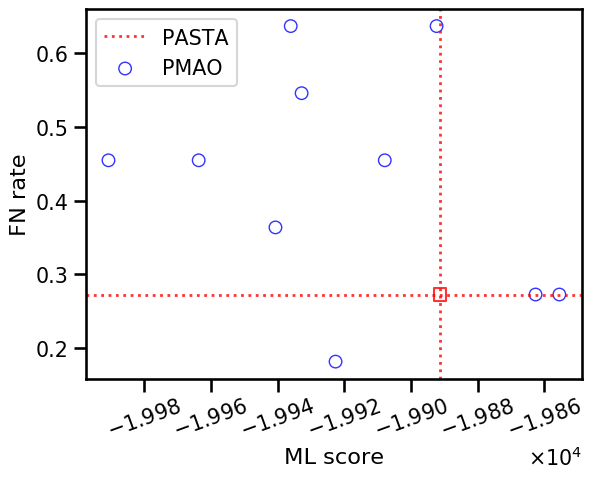
\includegraphics[width=0.22\textwidth]{PMAO-A/BB11018-fn-ml}}
\subfloat[BB12001]{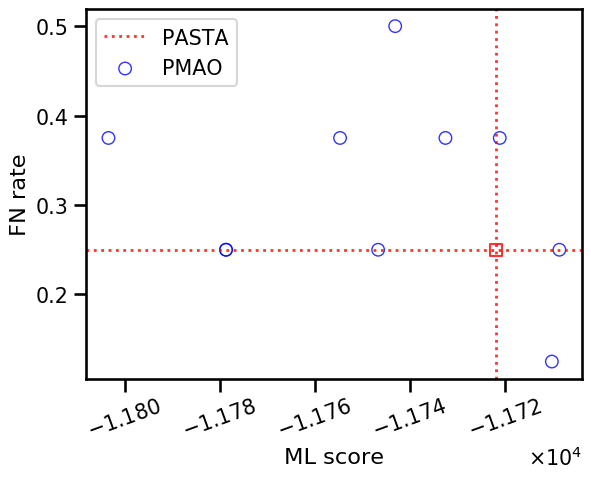
\includegraphics[width=0.22\textwidth]{PMAO-A/BB12001-fn-ml}}
\subfloat[BB20010]{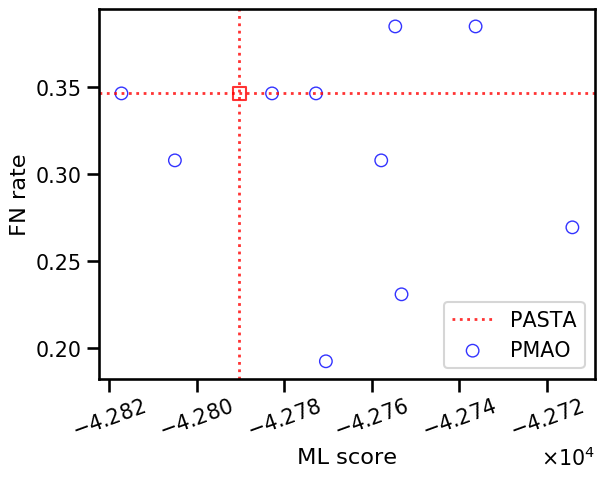
\includegraphics[width=0.22\textwidth]{PMAO-A/BB20010-fn-ml}}%
\subfloat[BB20041]{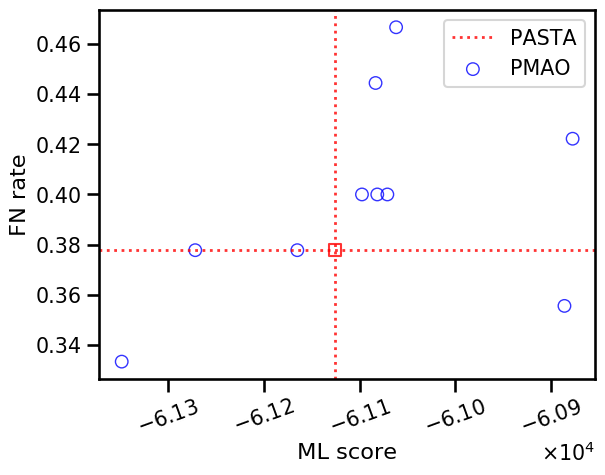
\includegraphics[width=0.22\textwidth]{PMAO-A/BB20041-fn-ml}}%
\subfloat[BB30002]{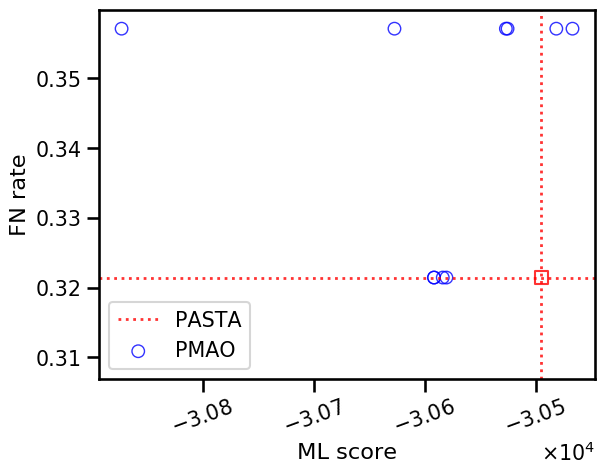
\includegraphics[width=0.22\textwidth]{PMAO-A/BB30002-fn-ml}}\\%
\subfloat[BB30008]{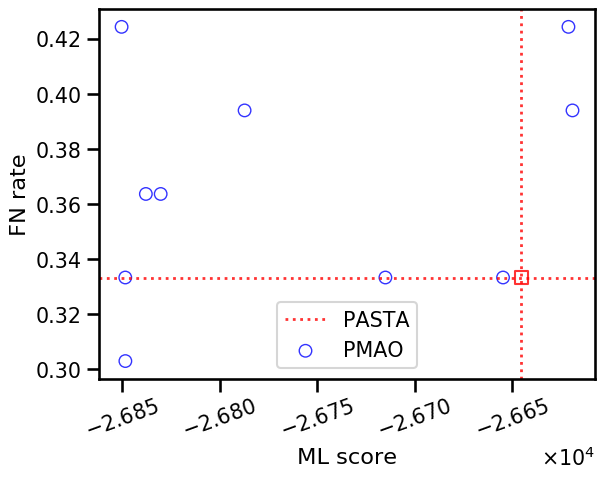
\includegraphics[width=0.22\textwidth]{PMAO-A/BB30008-fn-ml}}%
\subfloat[BB40001]{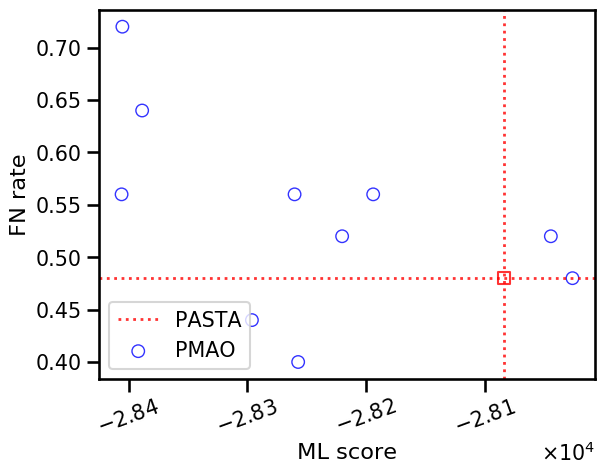
\includegraphics[width=0.22\textwidth]{PMAO-A/BB40001-fn-ml}}%
\subfloat[BB40048]{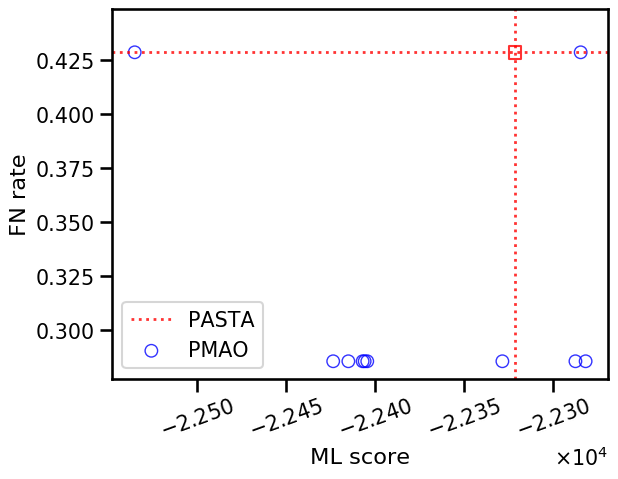
\includegraphics[width=0.22\textwidth]{PMAO-A/BB40048-fn-ml}}%
\subfloat[BB50005]{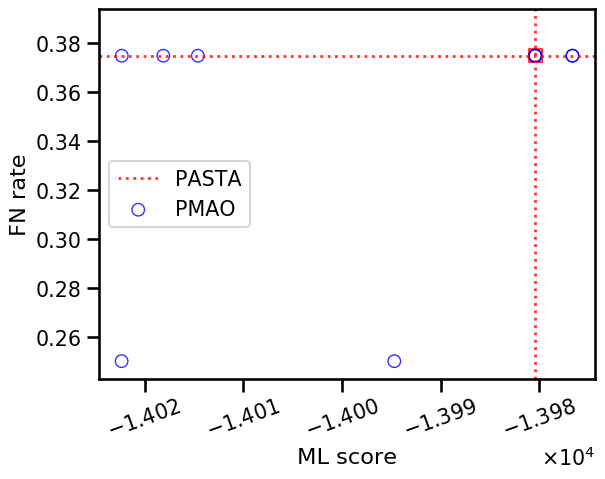
\includegraphics[width=0.22\textwidth]{PMAO-A/BB50005-fn-ml}}%	
\subfloat[BB50016]{\label{3figs-c}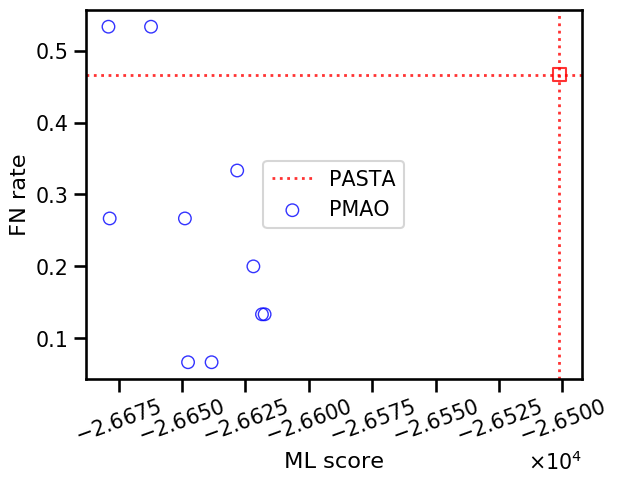
\includegraphics[width=0.22\textwidth]{PMAO-A/BB50016-fn-ml}}%
\end{adjustwidth}
\caption{Three sub-floats.}
\label{3figs}
\end{figure*}
\subsection{Dataset statistics}
\label{sec:dataset_stat}
% Table generated by Excel2LaTeX from sheet 'Sheet1'
\subsubsection{100-taxon simulated dataset}
We used five randomly selected replicates (R0, R4, R9, R14, R19) of simulated nucleotide dataset from the study of~\citealp{liu2009rapid}. It is publicly available at \url{https://sites.google.com/eng.ucsd.edu/datasets/sate-i}. Table~\ref{tab:sim_stat} gives the reference alignment statistics for this dataset.

\begin{table}[htbp]
	\centering
	\caption{Reference alignments for 100-taxon simulated dataset.}
	\begin{tabular}{|l|r|}
		\hline
		\multicolumn{1}{|c|}{Feature} & \multicolumn{1}{c|}{Value} \\
		\hline
		Number of taxa & 100 \\
		\hline
		Number of sites & 1698.2 \\
		\hline
		Percent indels & 40.4 \\
		\hline
		Avg. gap length & 3.1 \\
		\hline
	\end{tabular}%
	\label{tab:sim_stat}%
\end{table}%


\subsubsection{Biological rRNA datasets}
We analyzed two biological ribosomal RNA datasets, 23S.E and 23S.E.aa\_ag, from~\citealp{liu2009rapid} which are challenging for phylogeny estimation methods. Each of these datasets is given with a highly reliable, curated reference alignment from Gutell Lab. The statistics of the reference alignments of these datasets are presented in Table~\ref{tab:bio_stat}. Reference trees for these datasets were generated from the reference alignments by running RAxML~\citep{stamatakis2014raxml} with bootstrapping, and retaining only the highly supported edges. We evaluated generated alignments with respect to the reference alignment using the tool FastSP \citep{mirarab2011fastsp}.
% Table generated by Excel2LaTeX from sheet 'Sheet2'
\begin{table}[htbp]
	\small
	\centering
	\caption{Reference alignments for two biological rRNA datasets.}
	\begin{tabular}{|l|r|r|}
		\hline
		\multicolumn{1}{|c|}{Feature} & \multicolumn{1}{c|}{23S.E.aa\_ag} & \multicolumn{1}{c|}{23S.E} \\
		\hline
		Number of taxa & 144   & 117 \\
		\hline
		Number of sites & 8,619 & 9,079 \\
		\hline
		Percent indels & 61.1  & 59.7 \\
		\hline
		Avg. gap length & 13.5  & 12.6 \\
		\hline
	\end{tabular}%
	\label{tab:bio_stat}%
\end{table}%

\subsubsection{BAliBASE datasets}\label{subsec:balibase_stat}
BAliBASE 3.0 \citep{thompson2005balibase} is the most widely used benchmark alignment databases of protein families. It provides manually refined reference alignments of high quality based on 3D structural superposition. These datasets are organized into six groups according to their families and similarities: RV11 (very divergent sequences, residue identity below 20\% ), RV12 (medium to divergent sequences, 20\%-40\% residue identity), RV20 (families with one or more highly divergent sequences), RV30 (divergent subfamilies), RV40 (sequences with large terminal N/C extensions), and RV50 (sequences with large internal insertions). In this study, we selected four to five representative datasets from each group as reported in Table~\ref{tab:balibase}. We generated reference trees for these datasets by running RAxML~\citep{stamatakis2014raxml} with bootstrapping. We evaluated estimated alignments with respect to the core blocks (regions for which reliable alignments are known to exist) using the program bali\_score available at~\url{http://www.lbgi.fr/balibase/BalibaseDownload/}.

% Table generated by Excel2LaTeX from sheet 'Sheet2'
\begin{table}[htbp]
	\small
	\centering
	\caption{ BAliBASE datasets selected for this study.}
	\begin{tabular}{|l|l|}
		\hline
		\multicolumn{1}{|c|}{Group} & \multicolumn{1}{c|}{Datasets selected} \\
		\hline
		RV11  & BB11005, BB11018, BB11020, BB11033 \\
		\hline
		RV12  & BB12001, BB12013, BB12022, BB12035, BB12044 \\
		\hline
		RV20  & BB20001, BB20010, BB20022, BB20033, BB20041 \\
		\hline
		RV30  & BB30002, BB30008, BB30015, BB30022 \\
		\hline
		RV40  & BB40001, BB40013, BB40025, BB40038, BB40048 \\ %
		\hline
		RV50  & BB50001, BB50005, BB50010, BB50016 \\
		\hline
	\end{tabular}%
	\label{tab:balibase}%
\end{table}%

\subsection{Selection of appropriate multi-objective formulations}
\textit{(The following should be read in conjunction with the description presented in Section~\ref{sec:selection_msa_formulation} of the main text)} 

We visualize the interrelations among the objective values of the solutions, obtained by running NSGA-III to optimizes the objective set \{Gap, SOP, wSOP, TC\} on five randomly selected replicates (R0, R4, R9, R14, R19) of 100-taxon simulated dataset, using a $ 4\times4 $ scatter-plot matrix~\cite{kalyanmoy2001multi} as shown in Figure~\ref{fig:nature_obj}. Here each diagonal cell of a matrix depicts the distribution of the values of an objective function estimated using kernel density estimation which is a non-parametric way to estimate the probability density function of a random variable. And the non-diagonal cells show the correlation between each pair of objective functions. As our evolutionary algorithms tries to minimize all objective functions, we treat the maximization objective values by multiplying with -1. In the sequel, we normalize all the objective values using min-max technique and as such the maximization objectives are turned into minimization ones.

We estimate the coefficients of multiple linear regression model associating FN rate with each of the objective function from \{Gap, SOP, wSOP, TC\} using least-squares method and illustrate them using partial regression plots~\citep{montgomery2012introduction} in Figure~\ref{fig:mul_lin_reg}. We apply $t$-test on individual regression coefficient (i.e., slope) $\beta_i$ (with null hypothesis $\beta_i=0$) to test the significance of that association. The test results (slope, $p$-value) are incorporated in the figure.

We measure the strength of each objective set based on the FN rate achieved by the members of generated solution set. To accomplish this, For each set of objective functions, we run NSGA-II~\citep{deb2002fast} for 20 times following the standard practice of operations research (OR) literature (due to the stochastic nature of metaheuristics). Each run generates a set of solutions that represents the trade-offs in satisfying all objectives. Afterwards, we inferred ML tree for each of the generated alignment. We collected the best FN rates from each of the 20 solution sets and describe the distribution of these FN rates using boxplots which are shown in Figure~\ref{fig:rank_best_fn_rate}. In these boxplots we also incorporate the FN rates achieved by the state-of-the-art tools for comparison using horizontal lines.

\begin{figure*}[!htbp]	
	\begin{adjustwidth}{-1cm}{-1cm}
		\centering
		\begin{subfigure}{0.35\textwidth}
			\includegraphics[width=\columnwidth]{Figure/NumGaps_SOP_TC_wSOP/precomputedInit/R0/fig/scatter_mattrix}
			\caption{R0}
			%\label{fig:con_pr09}
		\end{subfigure}	
		\begin{subfigure}{0.35\textwidth}
			\includegraphics[width=\columnwidth]{Figure/NumGaps_SOP_TC_wSOP/precomputedInit/R4/fig/scatter_mattrix}
			\caption{R4}
			%\label{fig:con_pr09}
		\end{subfigure}
		\begin{subfigure}{0.35\textwidth}
			\includegraphics[width=\columnwidth]{Figure/NumGaps_SOP_TC_wSOP/precomputedInit/R9/fig/scatter_mattrix}
			\caption{R9}
			%\label{fig:con_pr09}
		\end{subfigure}
		\begin{subfigure}{0.35\textwidth}
			\includegraphics[width=\columnwidth]{Figure/NumGaps_SOP_TC_wSOP/precomputedInit/R14/fig/scatter_mattrix}
			\caption{R14}
			%\label{fig:con_pr09}
		\end{subfigure}
		\begin{subfigure}{0.35\textwidth}
			\includegraphics[width=\columnwidth]{Figure/NumGaps_SOP_TC_wSOP/precomputedInit/R19/fig/scatter_mattrix}
			\caption{R19}
			%\label{fig:con_pr09}
		\end{subfigure}
		\caption{\underline{100-taxon simulated dataset:} Scatter-plot matrices depicting the pairwise relationship of all objective functions on five randomly selected replicates. We turn each objective function into minimization form and then normalize using min-max technique. In each matrix, the diagonal cells show the distribution of objective values (estimated using kernel density estimation which is a non-parametric way to estimate the probability density function of a random variable) while the non-diagonal cells show the correlation between pairs of objective functions. Each upper-diagonal cell contains the value of correlation coefficient $r$ of the corresponding pair of objective functions.}
		\label{fig:nature_obj}
	\end{adjustwidth}
\end{figure*}

\begin{figure*}[!htbp]
	\centering
	\small
	\begin{adjustwidth}{-1cm}{-1cm}
		\begin{tabular}{l||C{0.24\textwidth}|C{0.24\textwidth}|C{0.24\textwidth}|C{0.24\textwidth} }
			& TC & Gap & SOP & wSOP\\\hline\hline
			\rotatebox[origin=c]{-90}{R0} & 
			\raisebox{-.5\height}{\includegraphics[width=0.25\textwidth]{Figure/NumGaps_SOP_TC_wSOP/precomputedInit/R0/fig/tc_partial_regression}} &
			\raisebox{-.5\height}{\includegraphics[width=0.25\textwidth]{Figure/NumGaps_SOP_TC_wSOP/precomputedInit/R0/fig/gap_partial_regression}} & 
			\raisebox{-.5\height}{\includegraphics[width=0.25\textwidth]{Figure/NumGaps_SOP_TC_wSOP/precomputedInit/R0/fig/sop_partial_regression}} & 
			\raisebox{-.5\height}{\includegraphics[width=0.25\textwidth]{Figure/NumGaps_SOP_TC_wSOP/precomputedInit/R0/fig/wsop_partial_regression}} 	
			\\\hline
			\rotatebox[origin=c]{-90}{R4} &
			\raisebox{-.5\height}{\includegraphics[width=0.25\textwidth]{Figure/NumGaps_SOP_TC_wSOP/precomputedInit/R4/fig/tc_partial_regression}} &
			\raisebox{-.5\height}{\includegraphics[width=0.25\textwidth]{Figure/NumGaps_SOP_TC_wSOP/precomputedInit/R4/fig/gap_partial_regression}} & 
			\raisebox{-.5\height}{\includegraphics[width=0.25\textwidth]{Figure/NumGaps_SOP_TC_wSOP/precomputedInit/R4/fig/sop_partial_regression}} & 
			\raisebox{-.5\height}{\includegraphics[width=0.25\textwidth]{Figure/NumGaps_SOP_TC_wSOP/precomputedInit/R4/fig/wsop_partial_regression}}
			\\\hline
			\rotatebox[origin=c]{-90}{R9} &
			\raisebox{-.5\height}{\includegraphics[width=0.25\textwidth]{Figure/NumGaps_SOP_TC_wSOP/precomputedInit/R9/fig/tc_partial_regression}} &
			\raisebox{-.5\height}{\includegraphics[width=0.25\textwidth]{Figure/NumGaps_SOP_TC_wSOP/precomputedInit/R9/fig/gap_partial_regression}} & 
			\raisebox{-.5\height}{\includegraphics[width=0.25\textwidth]{Figure/NumGaps_SOP_TC_wSOP/precomputedInit/R9/fig/sop_partial_regression}} & 
			\raisebox{-.5\height}{\includegraphics[width=0.25\textwidth]{Figure/NumGaps_SOP_TC_wSOP/precomputedInit/R9/fig/wsop_partial_regression}}
			\\\hline
			\rotatebox[origin=c]{-90}{R14} &
			\raisebox{-.5\height}{\includegraphics[width=0.25\textwidth]{Figure/NumGaps_SOP_TC_wSOP/precomputedInit/R14/fig/tc_partial_regression}} &
			\raisebox{-.5\height}{\includegraphics[width=0.25\textwidth]{Figure/NumGaps_SOP_TC_wSOP/precomputedInit/R14/fig/gap_partial_regression}} & 
			\raisebox{-.5\height}{\includegraphics[width=0.25\textwidth]{Figure/NumGaps_SOP_TC_wSOP/precomputedInit/R14/fig/sop_partial_regression}} & 
			\raisebox{-.5\height}{\includegraphics[width=0.25\textwidth]{Figure/NumGaps_SOP_TC_wSOP/precomputedInit/R14/fig/wsop_partial_regression}}
			\\\hline
			\rotatebox[origin=c]{-90}{R19} &
			\raisebox{-.5\height}{\includegraphics[width=0.25\textwidth]{Figure/NumGaps_SOP_TC_wSOP/precomputedInit/R19/fig/tc_partial_regression}} &
			\raisebox{-.5\height}{\includegraphics[width=0.25\textwidth]{Figure/NumGaps_SOP_TC_wSOP/precomputedInit/R19/fig/gap_partial_regression}} & 
			\raisebox{-.5\height}{\includegraphics[width=0.25\textwidth]{Figure/NumGaps_SOP_TC_wSOP/precomputedInit/R19/fig/sop_partial_regression}} & 
			\raisebox{-.5\height}{\includegraphics[width=0.25\textwidth]{Figure/NumGaps_SOP_TC_wSOP/precomputedInit/R19/fig/wsop_partial_regression}}
			\\\hline
		\end{tabular}
		\caption{\underline{100-taxon simulated dataset:} Multiple linear regression model for identifying the association among FN rate and three objective functions (TC, Gap and SOP/wSOP) fitted to five randomly selected replicates. There is one figure for each possible combination (replicate, objective function). Each partial regression plot shows the association between an objective function and FN rate while holding the remaining two objectives constant. In a plot for an objective function $ OF $, the horizontal axis, $e(OF|X)$, denotes the residuals from regressing $OF$ against the remaining objective functions and the vertical axis, $e(FNRate|X)$, denotes the residuals from regressing FN rate against all the objective functions except $ OF $.} 
		\label{fig:mul_lin_reg}
	\end{adjustwidth}
\end{figure*}

\begin{figure*}[!htbp]
	\centering
	\begin{adjustwidth}{-1cm}{-1cm}
		\begin{subfigure}{0.22\textwidth}
			\includegraphics[width=\columnwidth]{Figure/summary/precomputedInit/R0/objset_fnrate_rank}
			\caption{R0}
			%\label{fig:con_pr09}
		\end{subfigure}	
		\begin{subfigure}{0.22\textwidth}
			\includegraphics[width=\columnwidth]{Figure/summary/precomputedInit/R4/objset_fnrate_rank}
			\caption{R4}
			%\label{fig:con_pr09}
		\end{subfigure}
		\begin{subfigure}{0.22\textwidth}
			\includegraphics[width=\columnwidth]{Figure/summary/precomputedInit/R9/objset_fnrate_rank}
			\caption{R9}
			%\label{fig:con_pr09}
		\end{subfigure}
		\begin{subfigure}{0.22\textwidth}
			\includegraphics[width=\columnwidth]{Figure/summary/precomputedInit/R14/objset_fnrate_rank}
			\caption{R14}
			%\label{fig:con_pr09}
		\end{subfigure}
		\begin{subfigure}{0.22\textwidth}
			\includegraphics[width=\columnwidth]{Figure/summary/precomputedInit/R19/objset_fnrate_rank}
			\caption{R19}
			%\label{fig:con_pr09}
		\end{subfigure}
		\caption{\underline{100-taxon simulated dataset:} Comparison among objective sets based on the distribution of the collection of the best FN rates from each run. The performance of the state-of-the-art tools are shown using horizontal lines.}
		\label{fig:rank_best_fn_rate}
	\end{adjustwidth}
\end{figure*}


\begin{figure*}[!htbp]	
	\begin{adjustwidth}{-1cm}{-1cm}
		\centering
		\begin{subfigure}{0.35\textwidth}
			\includegraphics[width=\columnwidth]{Figure/6-obj-old/R0/fig/scatter_mattrix}
			\caption{R0}
			%\label{fig:con_pr09}
		\end{subfigure}	
		\begin{subfigure}{0.35\textwidth}
			\includegraphics[width=\columnwidth]{Figure/6-obj-old/R4/fig/scatter_mattrix}
			\caption{R4}
			%\label{fig:con_pr09}
		\end{subfigure}
		\begin{subfigure}{0.35\textwidth}
			\includegraphics[width=\columnwidth]{Figure/6-obj-old/R9/fig/scatter_mattrix}
			\caption{R9}
			%\label{fig:con_pr09}
		\end{subfigure}
		\begin{subfigure}{0.35\textwidth}
			\includegraphics[width=\columnwidth]{Figure/6-obj-old/R14/fig/scatter_mattrix}
			\caption{R14}
			%\label{fig:con_pr09}
		\end{subfigure}
		\begin{subfigure}{0.35\textwidth}
			\includegraphics[width=\columnwidth]{Figure/6-obj-old/R19/fig/scatter_mattrix}
			\caption{R19}
			%\label{fig:con_pr09}
		\end{subfigure}
		\caption{\underline{100-taxon simulated dataset:} Scatter-plot matrices depicting the pairwise relationship of all objective functions on five randomly selected replicates. We turn each objective function into minimization form and then normalize using min-max technique. In each matrix, the diagonal cells show the distribution of objective values (estimated using kernel density estimation which is a non-parametric way to estimate the probability density function of a random variable) while the non-diagonal cells show the correlation between pairs of objective functions. Each upper-diagonal cell contains the value of correlation coefficient $r$ of the corresponding pair of objective functions.}
		\label{fig:new_nature_obj}
	\end{adjustwidth}
\end{figure*}
\begin{figure*}[!htbp]
	\centering
	\small
	\begin{adjustwidth}{-1cm}{-1cm}
		\begin{tabular}{l||C{0.24\textwidth}|C{0.24\textwidth}|C{0.24\textwidth}|C{0.24\textwidth} }
			& Entropy & GapCon & SimG & SimNG\\\hline\hline
			\rotatebox[origin=c]{-90}{R0} & 
			\raisebox{-.5\height}{\includegraphics[width=0.25\textwidth]{Figure/6-obj-old/precomputedInit/R0/fig/Entropy_partial_regression}} &
			\raisebox{-.5\height}{\includegraphics[width=0.25\textwidth]{Figure/6-obj-old/precomputedInit/R0/fig/GapCon_partial_regression}} & 
			\raisebox{-.5\height}{\includegraphics[width=0.25\textwidth]{Figure/6-obj-old/precomputedInit/R0/fig/SimG_partial_regression}} & 
			\raisebox{-.5\height}{\includegraphics[width=0.25\textwidth]{Figure/6-obj-old/precomputedInit/R0/fig/SimNG_partial_regression}} 	
			\\\hline
			\rotatebox[origin=c]{-90}{R4} &
			\raisebox{-.5\height}{\includegraphics[width=0.25\textwidth]{Figure/6-obj-old/precomputedInit/R4/fig/Entropy_partial_regression}} &
			\raisebox{-.5\height}{\includegraphics[width=0.25\textwidth]{Figure/6-obj-old/precomputedInit/R4/fig/GapCon_partial_regression}} & 
			\raisebox{-.5\height}{\includegraphics[width=0.25\textwidth]{Figure/6-obj-old/precomputedInit/R4/fig/SimG_partial_regression}} & 
			\raisebox{-.5\height}{\includegraphics[width=0.25\textwidth]{Figure/6-obj-old/precomputedInit/R4/fig/SimNG_partial_regression}}
			\\\hline
			\rotatebox[origin=c]{-90}{R9} &
			\raisebox{-.5\height}{\includegraphics[width=0.25\textwidth]{Figure/6-obj-old/precomputedInit/R9/fig/Entropy_partial_regression}} &
			\raisebox{-.5\height}{\includegraphics[width=0.25\textwidth]{Figure/6-obj-old/precomputedInit/R9/fig/GapCon_partial_regression}} & 
			\raisebox{-.5\height}{\includegraphics[width=0.25\textwidth]{Figure/6-obj-old/precomputedInit/R9/fig/SimG_partial_regression}} & 
			\raisebox{-.5\height}{\includegraphics[width=0.25\textwidth]{Figure/6-obj-old/precomputedInit/R9/fig/SimNG_partial_regression}}
			\\\hline
			\rotatebox[origin=c]{-90}{R14} &
			\raisebox{-.5\height}{\includegraphics[width=0.25\textwidth]{Figure/6-obj-old/precomputedInit/R14/fig/Entropy_partial_regression}} &
			\raisebox{-.5\height}{\includegraphics[width=0.25\textwidth]{Figure/6-obj-old/precomputedInit/R14/fig/GapCon_partial_regression}} & 
			\raisebox{-.5\height}{\includegraphics[width=0.25\textwidth]{Figure/6-obj-old/precomputedInit/R14/fig/SimG_partial_regression}} & 
			\raisebox{-.5\height}{\includegraphics[width=0.25\textwidth]{Figure/6-obj-old/precomputedInit/R14/fig/SimNG_partial_regression}}
			\\\hline
			\rotatebox[origin=c]{-90}{R19} &
			\raisebox{-.5\height}{\includegraphics[width=0.25\textwidth]{Figure/6-obj-old/precomputedInit/R19/fig/Entropy_partial_regression}} &
			\raisebox{-.5\height}{\includegraphics[width=0.25\textwidth]{Figure/6-obj-old/precomputedInit/R19/fig/GapCon_partial_regression}} & 
			\raisebox{-.5\height}{\includegraphics[width=0.25\textwidth]{Figure/6-obj-old/precomputedInit/R19/fig/SimG_partial_regression}} & 
			\raisebox{-.5\height}{\includegraphics[width=0.25\textwidth]{Figure/6-obj-old/precomputedInit/R19/fig/SimNG_partial_regression}}
			\\\hline
		\end{tabular}	
		\caption{\underline{100-taxon simulated dataset:} Multiple linear regression model for identifying the association among FN rate and three objective functions (SimNG, GapCon and SimG/Entropy) fitted to five randomly selected replicates. There is one figure for each possible combination (replicate, objective function). Each partial regression plot shows the association between an objective function and FN rate while holding the remaining two objectives constant.  In a plot for an objective function $ OF $, the horizontal axis, $e(OF|X)$, denotes the residuals from regressing $OF$ against the remaining objective functions and the vertical axis, $e(FNRate|X)$, denotes the residuals from regressing FN rate against all the objective functions except $ OF $.}
		\label{fig:new_mul_lin_reg}
	\end{adjustwidth}
\end{figure*}
\clearpage
\subsection{Further results on BAliBASE datasets}
Here we first discuss our findings for the five datasets under group RV12. Here According to FN rate (Figure \ref{fig:rv12_fn_rate}), the multi-objective formulations outperform all the state-of-the-art tools for BB12013 and BB12035. In case of BB12035, \{SimG, SimNG\} reconstructs all the edges correctly as opposed to 20\% FN rate attained by the trees estimated on the MSA generated by the best tool which is remarkable.
%shows remarkable improvement in FN rate \commentA{(0\% vs 20\%)}\footnote{\commentA{Here I mean, our approach achieves 0\% FN rate while the best tool achieves 20\% Fn rate}} compared to the best tool. 
For the remaining datasets (BB12001 and BB12022), the multi-objective formulations perform as good as the best tool. On all the datasets, the two objective sets generate several solutions that are equivalent or better than that of the best tool.
%the two objective sets generate several solutions that are similar to or better than the best tool on all the datasets. And the set \{SimG, SimNG\} performs better than \{Gap, SOP\} except for BB12044. 
However, as observed in previous datasets, we see contrasting results with respect to TC and SP score (Figure \ref{fig:rv12_tc},\ref{fig:rv12_sp}). Here we find only a few cases where the two objective sets can outperform the best tool. We closely analyze this issue in Figure~\ref{fig:rv12_fnrate_vs_tc} where we find that there are several solutions that achieve better FN rates in spite of their poor alignment quality (TC and SP score). For the remaining groups, our obtained results are similar. For the sake of brevity, we only illustrate the results in Figures \ref{fig:rv20_fn_rate} to \ref{fig:rv50_fnrate_vs_tc}.
%############################# RV12
\begin{figure*}[!htbp]
	\centering
	\begin{adjustwidth}{-1cm}{-1cm}
		\begin{subfigure}{0.22\textwidth}
			\includegraphics[width=\columnwidth]{Figure/summary/precomputedInit/Balibase/BB12001_fnrate_density_single_run}
			\caption{BB12001}
			%\label{fig:con_pr09}
		\end{subfigure}	
		\begin{subfigure}{0.22\textwidth}
			\includegraphics[width=\columnwidth]{Figure/summary/precomputedInit/Balibase/BB12013_fnrate_density_single_run}
			\caption{BB12013}
			%\label{fig:con_pr09}
		\end{subfigure}
		\begin{subfigure}{0.22\textwidth}
			\includegraphics[width=\columnwidth]{Figure/summary/precomputedInit/Balibase/BB12022_fnrate_density_single_run}
			\caption{BB12022}
			%\label{fig:con_pr09}
		\end{subfigure}
		\begin{subfigure}{0.22\textwidth}
			\includegraphics[width=\columnwidth]{Figure/summary/precomputedInit/Balibase/BB12035_fnrate_density_single_run}
			\caption{BB12035}
			%\label{fig:con_pr09}
		\end{subfigure}
		\begin{subfigure}{0.22\textwidth}
			\includegraphics[width=\columnwidth]{Figure/summary/precomputedInit/Balibase/BB12044_fnrate_density_single_run}
			\caption{BB12044}
			%\label{fig:con_pr09}
		\end{subfigure}
		\begin{subfigure}{0.22\textwidth}
			\includegraphics[width=\columnwidth]{Figure/summary/precomputedInit/Balibase/BB12001_objset_fnrate_rank}
			\caption{BB12001}
			%\label{fig:con_pr09}
		\end{subfigure}	
		\begin{subfigure}{0.22\textwidth}
			\includegraphics[width=\columnwidth]{Figure/summary/precomputedInit/Balibase/BB12013_objset_fnrate_rank}
			\caption{BB12013}
			%\label{fig:con_pr09}
		\end{subfigure}
		\begin{subfigure}{0.22\textwidth}
			\includegraphics[width=\columnwidth]{Figure/summary/precomputedInit/Balibase/BB12022_objset_fnrate_rank}
			\caption{BB12022}
			%\label{fig:con_pr09}
		\end{subfigure}
		\begin{subfigure}{0.22\textwidth}
			\includegraphics[width=\columnwidth]{Figure/summary/precomputedInit/Balibase/BB12035_objset_fnrate_rank}
			\caption{BB12035}
			%\label{fig:con_pr09}
		\end{subfigure}
		\begin{subfigure}{0.22\textwidth}
			\includegraphics[width=\columnwidth]{Figure/summary/precomputedInit/Balibase/BB12044_objset_fnrate_rank}
			\caption{BB12044}
			%\label{fig:con_pr09}
		\end{subfigure}
		\caption{\underline{RV12:} Top panel (part (a) - (e)) shows the FN rate of 100 solutions averaged over 20 runs. At first, we sort the FN rates of each solution set. Then we average the FN rates at each sorted position of all the sets. Bottom panel (part (f) - (j)) shows the distribution of the best FN rates collected from all runs. In each figure, the horizontal lines show the performance of the state-of-the-art tools.}
		\label{fig:rv12_fn_rate}
	\end{adjustwidth}
\end{figure*}


\begin{figure*}[!htbp]
	\centering
	\begin{adjustwidth}{-1cm}{-1cm}
		\begin{subfigure}{0.22\textwidth}
			\includegraphics[width=\columnwidth]{Figure/summary/precomputedInit/Balibase/BB12001_tc_density_single_run_2}
			\caption{BB12001}
			%\label{fig:con_pr09}
		\end{subfigure}	
		\begin{subfigure}{0.22\textwidth}
			\includegraphics[width=\columnwidth]{Figure/summary/precomputedInit/Balibase/BB12013_tc_density_single_run_2}
			\caption{BB12013}
			%\label{fig:con_pr09}
		\end{subfigure}
		\begin{subfigure}{0.22\textwidth}
			\includegraphics[width=\columnwidth]{Figure/summary/precomputedInit/Balibase/BB12022_tc_density_single_run_2}
			\caption{BB12022}
			%\label{fig:con_pr09}
		\end{subfigure}
		\begin{subfigure}{0.22\textwidth}
			\includegraphics[width=\columnwidth]{Figure/summary/precomputedInit/Balibase/BB12035_tc_density_single_run_2}
			\caption{BB12035}
			%\label{fig:con_pr09}
		\end{subfigure}
		\begin{subfigure}{0.22\textwidth}
			\includegraphics[width=\columnwidth]{Figure/summary/precomputedInit/Balibase/BB12044_tc_density_single_run_2}
			\caption{BB12044}
			%\label{fig:con_pr09}
		\end{subfigure}
		%%%%%%%%%%%%%%
		\begin{subfigure}{0.22\textwidth}
			\includegraphics[width=\columnwidth]{Figure/summary/precomputedInit/Balibase/BB12001_objset_tc_rank_2}
			\caption{BB12001}
			%\label{fig:con_pr09}
		\end{subfigure}	
		\begin{subfigure}{0.22\textwidth}
			\includegraphics[width=\columnwidth]{Figure/summary/precomputedInit/Balibase/BB12013_objset_tc_rank_2}
			\caption{BB12013}
			%\label{fig:con_pr09}
		\end{subfigure}
		\begin{subfigure}{0.22\textwidth}
			\includegraphics[width=\columnwidth]{Figure/summary/precomputedInit/Balibase/BB12022_objset_tc_rank_2}
			\caption{BB12022}
			%\label{fig:con_pr09}
		\end{subfigure}
		\begin{subfigure}{0.22\textwidth}
			\includegraphics[width=\columnwidth]{Figure/summary/precomputedInit/Balibase/BB12035_objset_tc_rank_2}
			\caption{BB12035}
			%\label{fig:con_pr09}
		\end{subfigure}
		\begin{subfigure}{0.22\textwidth}
			\includegraphics[width=\columnwidth]{Figure/summary/precomputedInit/Balibase/BB12044_objset_tc_rank_2}
			\caption{BB12044}
			%\label{fig:con_pr09}
		\end{subfigure}
		\caption{\underline{RV12:} Top panel (part (a) - (e)) shows the TC score of 100 solutions averaged over 20 runs. At first, we sort the TC scores of each solution set. Then we average the TC scores at each sorted position of all the sets. Bottom panel (part (f) - (j)) shows the distribution of the best TC scores collected from all runs. In each figure, the horizontal lines show the performance of the state-of-the-art tools.}
		\label{fig:rv12_tc}
	\end{adjustwidth}
\end{figure*}


\begin{figure*}[!htbp]
	\centering
	\begin{adjustwidth}{-1cm}{-1cm}
		\begin{subfigure}{0.22\textwidth}
			\includegraphics[width=\columnwidth]{Figure/summary/precomputedInit/Balibase/BB12001_pairs_density_single_run_2}
			\caption{BB12001}
			%\label{fig:con_pr09}
		\end{subfigure}	
		\begin{subfigure}{0.22\textwidth}
			\includegraphics[width=\columnwidth]{Figure/summary/precomputedInit/Balibase/BB12013_pairs_density_single_run_2}
			\caption{BB12013}
			%\label{fig:con_pr09}
		\end{subfigure}
		\begin{subfigure}{0.22\textwidth}
			\includegraphics[width=\columnwidth]{Figure/summary/precomputedInit/Balibase/BB12022_pairs_density_single_run_2}
			\caption{BB12022}
			%\label{fig:con_pr09}
		\end{subfigure}
		\begin{subfigure}{0.22\textwidth}
			\includegraphics[width=\columnwidth]{Figure/summary/precomputedInit/Balibase/BB12035_pairs_density_single_run_2}
			\caption{BB12035}
			%\label{fig:con_pr09}
		\end{subfigure}
		\begin{subfigure}{0.22\textwidth}
			\includegraphics[width=\columnwidth]{Figure/summary/precomputedInit/Balibase/BB12044_pairs_density_single_run_2}
			\caption{BB12044}
			%\label{fig:con_pr09}
		\end{subfigure}
		\begin{subfigure}{0.22\textwidth}
			\includegraphics[width=\columnwidth]{Figure/summary/precomputedInit/Balibase/BB12001_objset_pairs_rank_2}
			\caption{BB12001}
			%\label{fig:con_pr09}
		\end{subfigure}	
		\begin{subfigure}{0.22\textwidth}
			\includegraphics[width=\columnwidth]{Figure/summary/precomputedInit/Balibase/BB12013_objset_pairs_rank_2}
			\caption{BB12013}
			%\label{fig:con_pr09}
		\end{subfigure}
		\begin{subfigure}{0.22\textwidth}
			\includegraphics[width=\columnwidth]{Figure/summary/precomputedInit/Balibase/BB12022_objset_pairs_rank_2}
			\caption{BB12022}
			%\label{fig:con_pr09}
		\end{subfigure}
		\begin{subfigure}{0.22\textwidth}
			\includegraphics[width=\columnwidth]{Figure/summary/precomputedInit/Balibase/BB12035_objset_pairs_rank_2}
			\caption{BB12035}
			%\label{fig:con_pr09}
		\end{subfigure}
		\begin{subfigure}{0.22\textwidth}
			\includegraphics[width=\columnwidth]{Figure/summary/precomputedInit/Balibase/BB12044_objset_pairs_rank_2}
			\caption{BB12044}
			%\label{fig:con_pr09}
		\end{subfigure}
		\caption{\underline{RV12:} Top panel (part (a) - (e)) shows the SP score of 100 solutions averaged over 20 runs. At first, we sort the SP scores of each solution set. Then we average the SP scores at each sorted position of all the sets. Bottom panel (part (f) - (j)) shows the distribution of the best SP scores collected from all runs. In each figure, the horizontal lines show the performance of the state-of-the-art tools.}
		\label{fig:rv12_sp}
	\end{adjustwidth}
\end{figure*}


\begin{figure*}[!htbp]
	\centering
	\begin{adjustwidth}{-1cm}{-1cm}
		\begin{subfigure}{0.22\textwidth}
			\includegraphics[width=\columnwidth]{Figure/summary/precomputedInit/Balibase/BB12001_fnrate_vs_tc_2}
			\caption{BB12001}
			%\label{fig:con_pr09}
		\end{subfigure}	
		\begin{subfigure}{0.22\textwidth}
			\includegraphics[width=\columnwidth]{Figure/summary/precomputedInit/Balibase/BB12013_fnrate_vs_tc_2}
			\caption{BB12013}
			%\label{fig:con_pr09}
		\end{subfigure}
		\begin{subfigure}{0.22\textwidth}
			\includegraphics[width=\columnwidth]{Figure/summary/precomputedInit/Balibase/BB12022_fnrate_vs_tc_2}
			\caption{BB12022}
			%\label{fig:con_pr09}
		\end{subfigure}
		\begin{subfigure}{0.22\textwidth}
			\includegraphics[width=\columnwidth]{Figure/summary/precomputedInit/Balibase/BB12035_fnrate_vs_tc_2}
			\caption{BB12035}
			%\label{fig:con_pr09}
		\end{subfigure}	
		\begin{subfigure}{0.22\textwidth}
			\includegraphics[width=\columnwidth]{Figure/summary/precomputedInit/Balibase/BB12044_fnrate_vs_tc_2}
			\caption{BB12044}
			%\label{fig:con_pr09}
		\end{subfigure}
		%%%%%%%%%
		\begin{subfigure}{0.22\textwidth}
			\includegraphics[width=\columnwidth]{Figure/summary/precomputedInit/Balibase/BB12001_fnrate_vs_sp_2}
			\caption{BB12001}
			%\label{fig:con_pr09}
		\end{subfigure}	
		\begin{subfigure}{0.22\textwidth}
			\includegraphics[width=\columnwidth]{Figure/summary/precomputedInit/Balibase/BB12013_fnrate_vs_sp_2}
			\caption{BB12013}
			%\label{fig:con_pr09}
		\end{subfigure}
		\begin{subfigure}{0.22\textwidth}
			\includegraphics[width=\columnwidth]{Figure/summary/precomputedInit/Balibase/BB12022_fnrate_vs_sp_2}
			\caption{BB12022}
			%\label{fig:con_pr09}
		\end{subfigure}
		\begin{subfigure}{0.22\textwidth}
			\includegraphics[width=\columnwidth]{Figure/summary/precomputedInit/Balibase/BB12035_fnrate_vs_sp_2}
			\caption{BB12035}
			%\label{fig:con_pr09}
		\end{subfigure}	
		\begin{subfigure}{0.22\textwidth}
			\includegraphics[width=\columnwidth]{Figure/summary/precomputedInit/Balibase/BB12044_fnrate_vs_sp_2}
			\caption{BB12044}
			%\label{fig:con_pr09}
		\end{subfigure}
		\caption{\underline{RV12}: Top panel (part (a) - (e)) shows the relationship between FN rate and TC score for different alignments. And bottom panel (part (f) - (j)) shows the relationship between FN rate and SP score. The horizontal lines mark the FN rates achieved by the state-of-the-art tools.}
		\label{fig:rv12_fnrate_vs_tc}
	\end{adjustwidth}
\end{figure*}
%############################# RV20
\begin{figure*}[!htbp]
	\centering
	\begin{adjustwidth}{-1cm}{-1cm}
		\begin{subfigure}{0.22\textwidth}
			\includegraphics[width=\columnwidth]{Figure/summary/precomputedInit/Balibase/BB20001_fnrate_density_single_run}
			\caption{BB20001}
			%\label{fig:con_pr09}
		\end{subfigure}	
		\begin{subfigure}{0.22\textwidth}
			\includegraphics[width=\columnwidth]{Figure/summary/precomputedInit/Balibase/BB20010_fnrate_density_single_run}
			\caption{BB20010}
			%\label{fig:con_pr09}
		\end{subfigure}
		\begin{subfigure}{0.22\textwidth}
			\includegraphics[width=\columnwidth]{Figure/summary/precomputedInit/Balibase/BB20022_fnrate_density_single_run}
			\caption{BB20022}
			%\label{fig:con_pr09}
		\end{subfigure}
		\begin{subfigure}{0.22\textwidth}
			\includegraphics[width=\columnwidth]{Figure/summary/precomputedInit/Balibase/BB20033_fnrate_density_single_run}
			\caption{BB20033}
			%\label{fig:con_pr09}
		\end{subfigure}
		\begin{subfigure}{0.22\textwidth}
			\includegraphics[width=\columnwidth]{Figure/summary/precomputedInit/Balibase/BB20041_fnrate_density_single_run}
			\caption{BB20041}
			%\label{fig:con_pr09}
		\end{subfigure}
		\begin{subfigure}{0.22\textwidth}
			\includegraphics[width=\columnwidth]{Figure/summary/precomputedInit/Balibase/BB20001_objset_fnrate_rank}
			\caption{BB20001}
			%\label{fig:con_pr09}
		\end{subfigure}	
		\begin{subfigure}{0.22\textwidth}
			\includegraphics[width=\columnwidth]{Figure/summary/precomputedInit/Balibase/BB20010_objset_fnrate_rank}
			\caption{BB20010}
			%\label{fig:con_pr09}
		\end{subfigure}
		\begin{subfigure}{0.22\textwidth}
			\includegraphics[width=\columnwidth]{Figure/summary/precomputedInit/Balibase/BB20022_objset_fnrate_rank}
			\caption{BB20022}
			%\label{fig:con_pr09}
		\end{subfigure}
		\begin{subfigure}{0.22\textwidth}
			\includegraphics[width=\columnwidth]{Figure/summary/precomputedInit/Balibase/BB20033_objset_fnrate_rank}
			\caption{BB20033}
			%\label{fig:con_pr09}
		\end{subfigure}
		\begin{subfigure}{0.22\textwidth}
			\includegraphics[width=\columnwidth]{Figure/summary/precomputedInit/Balibase/BB20041_objset_fnrate_rank}
			\caption{BB20041}
			%\label{fig:con_pr09}
		\end{subfigure}
		\caption{\underline{RV20:} Top panel (part (a) - (d)) shows the FN rate of 100 final solutions averaged over 20 runs. At first, we sort the FN rates of each solution set. Then we average the FN rates at each sorted position of all the sets. Bottom panel (part (e) - (h)) shows the distribution of the best FN rates collected from all runs. In each figure, the horizontal lines show the performance of the state-of-the-art tools.}
		\label{fig:rv20_fn_rate}
	\end{adjustwidth}
\end{figure*}


\begin{figure*}[!htbp]
	\centering
	\begin{adjustwidth}{-1cm}{-1cm}
		\begin{subfigure}{0.22\textwidth}
			\includegraphics[width=\columnwidth]{Figure/summary/precomputedInit/Balibase/BB20001_tc_density_single_run_2}
			\caption{BB20001}
			%\label{fig:con_pr09}
		\end{subfigure}	
		\begin{subfigure}{0.22\textwidth}
			\includegraphics[width=\columnwidth]{Figure/summary/precomputedInit/Balibase/BB20010_tc_density_single_run_2}
			\caption{BB20010}
			%\label{fig:con_pr09}
		\end{subfigure}
		\begin{subfigure}{0.22\textwidth}
			\includegraphics[width=\columnwidth]{Figure/summary/precomputedInit/Balibase/BB20022_tc_density_single_run_2}
			\caption{BB20022}
			%\label{fig:con_pr09}
		\end{subfigure}
		\begin{subfigure}{0.22\textwidth}
			\includegraphics[width=\columnwidth]{Figure/summary/precomputedInit/Balibase/BB20033_tc_density_single_run_2}
			\caption{BB20033}
			%\label{fig:con_pr09}
		\end{subfigure}
		\begin{subfigure}{0.22\textwidth}
			\includegraphics[width=\columnwidth]{Figure/summary/precomputedInit/Balibase/BB20041_tc_density_single_run_2}
			\caption{BB20041}
			%\label{fig:con_pr09}
		\end{subfigure}
		\begin{subfigure}{0.22\textwidth}
			\includegraphics[width=\columnwidth]{Figure/summary/precomputedInit/Balibase/BB20001_objset_tc_rank_2}
			\caption{BB20001}
			%\label{fig:con_pr09}
		\end{subfigure}	
		\begin{subfigure}{0.22\textwidth}
			\includegraphics[width=\columnwidth]{Figure/summary/precomputedInit/Balibase/BB20010_objset_tc_rank_2}
			\caption{BB20010}
			%\label{fig:con_pr09}
		\end{subfigure}
		\begin{subfigure}{0.22\textwidth}
			\includegraphics[width=\columnwidth]{Figure/summary/precomputedInit/Balibase/BB20022_objset_tc_rank_2}
			\caption{BB20022}
			%\label{fig:con_pr09}
		\end{subfigure}
		\begin{subfigure}{0.22\textwidth}
			\includegraphics[width=\columnwidth]{Figure/summary/precomputedInit/Balibase/BB20033_objset_tc_rank_2}
			\caption{BB20033}
			%\label{fig:con_pr09}
		\end{subfigure}
		\begin{subfigure}{0.22\textwidth}
			\includegraphics[width=\columnwidth]{Figure/summary/precomputedInit/Balibase/BB20041_objset_tc_rank_2}
			\caption{BB20041}
			%\label{fig:con_pr09}
		\end{subfigure}
		\caption{\underline{RV20:} Top panel (part (a) - (e)) shows the TC score of 100 final solutions averaged over 20 runs. At first, we sort the TC scores of each solution set. Then we average the TC scores at each sorted position of all the sets. Bottom panel (part (f) - (j)) shows the distribution of the best TC scores collected from all runs. In each figure, the horizontal lines show the performance of the state-of-the-art tools.}
		\label{fig:rv20_tc}
	\end{adjustwidth}
\end{figure*}

\begin{figure*}[!htbp]
	\centering
	\begin{adjustwidth}{-1cm}{-1cm}
		\begin{subfigure}{0.22\textwidth}
			\includegraphics[width=\columnwidth]{Figure/summary/precomputedInit/Balibase/BB20001_pairs_density_single_run_2}
			\caption{BB20001}
			%\label{fig:con_pr09}
		\end{subfigure}	
		\begin{subfigure}{0.22\textwidth}
			\includegraphics[width=\columnwidth]{Figure/summary/precomputedInit/Balibase/BB20010_pairs_density_single_run_2}
			\caption{BB20010}
			%\label{fig:con_pr09}
		\end{subfigure}
		\begin{subfigure}{0.22\textwidth}
			\includegraphics[width=\columnwidth]{Figure/summary/precomputedInit/Balibase/BB20022_pairs_density_single_run_2}
			\caption{BB20022}
			%\label{fig:con_pr09}
		\end{subfigure}
		\begin{subfigure}{0.22\textwidth}
			\includegraphics[width=\columnwidth]{Figure/summary/precomputedInit/Balibase/BB20033_pairs_density_single_run_2}
			\caption{BB20033}
			%\label{fig:con_pr09}
		\end{subfigure}
		\begin{subfigure}{0.22\textwidth}
			\includegraphics[width=\columnwidth]{Figure/summary/precomputedInit/Balibase/BB20041_pairs_density_single_run_2}
			\caption{BB20041}
			%\label{fig:con_pr09}
		\end{subfigure}
		\begin{subfigure}{0.22\textwidth}
			\includegraphics[width=\columnwidth]{Figure/summary/precomputedInit/Balibase/BB20001_objset_pairs_rank_2}
			\caption{BB20001}
			%\label{fig:con_pr09}
		\end{subfigure}	
		\begin{subfigure}{0.22\textwidth}
			\includegraphics[width=\columnwidth]{Figure/summary/precomputedInit/Balibase/BB20010_objset_pairs_rank_2}
			\caption{BB20010}
			%\label{fig:con_pr09}
		\end{subfigure}
		\begin{subfigure}{0.22\textwidth}
			\includegraphics[width=\columnwidth]{Figure/summary/precomputedInit/Balibase/BB20022_objset_pairs_rank_2}
			\caption{BB20022}
			%\label{fig:con_pr09}
		\end{subfigure}
		\begin{subfigure}{0.22\textwidth}
			\includegraphics[width=\columnwidth]{Figure/summary/precomputedInit/Balibase/BB20033_objset_pairs_rank_2}
			\caption{BB20033}
			%\label{fig:con_pr09}
		\end{subfigure}
		\begin{subfigure}{0.22\textwidth}
			\includegraphics[width=\columnwidth]{Figure/summary/precomputedInit/Balibase/BB20041_objset_pairs_rank_2}
			\caption{BB20041}
			%\label{fig:con_pr09}
		\end{subfigure}
		\caption{\underline{RV20:} Top panel (part (a) - (e)) shows the SP score of 100 final solutions averaged over 20 runs. At first, we sort the SP scores of each solution set. Then we average the SP scores at each sorted position of all the sets. Bottom panel (part (f) - (j)) shows the distribution of the best SP scores collected from all runs. In each figure, the horizontal lines show the performance of the state-of-the-art tools.}
		\label{fig:rv20_sp}
	\end{adjustwidth}
\end{figure*}


\begin{figure*}[!htbp]
	\centering
	\begin{adjustwidth}{-1cm}{-1cm}
		\begin{subfigure}{0.22\textwidth}
			\includegraphics[width=\columnwidth]{Figure/summary/precomputedInit/Balibase/BB20001_fnrate_vs_tc_2}
			\caption{BB20001}
			%\label{fig:con_pr09}
		\end{subfigure}	
		\begin{subfigure}{0.22\textwidth}
			\includegraphics[width=\columnwidth]{Figure/summary/precomputedInit/Balibase/BB20010_fnrate_vs_tc_2}
			\caption{BB20010}
			%\label{fig:con_pr09}
		\end{subfigure}
		\begin{subfigure}{0.22\textwidth}
			\includegraphics[width=\columnwidth]{Figure/summary/precomputedInit/Balibase/BB20022_fnrate_vs_tc_2}
			\caption{BB20022}
			%\label{fig:con_pr09}
		\end{subfigure}
		\begin{subfigure}{0.22\textwidth}
			\includegraphics[width=\columnwidth]{Figure/summary/precomputedInit/Balibase/BB20033_fnrate_vs_tc_2}
			\caption{BB20033}
			%\label{fig:con_pr09}
		\end{subfigure}	
		\begin{subfigure}{0.22\textwidth}
			\includegraphics[width=\columnwidth]{Figure/summary/precomputedInit/Balibase/BB20041_fnrate_vs_tc_2}
			\caption{BB20041}
			%\label{fig:con_pr09}
		\end{subfigure}
		%%%%%%%%%%
		\begin{subfigure}{0.22\textwidth}
			\includegraphics[width=\columnwidth]{Figure/summary/precomputedInit/Balibase/BB20001_fnrate_vs_sp_2}
			\caption{BB20001}
			%\label{fig:con_pr09}
		\end{subfigure}	
		\begin{subfigure}{0.22\textwidth}
			\includegraphics[width=\columnwidth]{Figure/summary/precomputedInit/Balibase/BB20010_fnrate_vs_sp_2}
			\caption{BB20010}
			%\label{fig:con_pr09}
		\end{subfigure}
		\begin{subfigure}{0.22\textwidth}
			\includegraphics[width=\columnwidth]{Figure/summary/precomputedInit/Balibase/BB20022_fnrate_vs_sp_2}
			\caption{BB20022}
			%\label{fig:con_pr09}
		\end{subfigure}
		\begin{subfigure}{0.22\textwidth}
			\includegraphics[width=\columnwidth]{Figure/summary/precomputedInit/Balibase/BB20033_fnrate_vs_sp_2}
			\caption{BB20033}
			%\label{fig:con_pr09}
		\end{subfigure}	
		\begin{subfigure}{0.22\textwidth}
			\includegraphics[width=\columnwidth]{Figure/summary/precomputedInit/Balibase/BB20041_fnrate_vs_sp_2}
			\caption{BB20041}
			%\label{fig:con_pr09}
		\end{subfigure}
		\caption{\underline{RV20:} Top panel (part (a) - (e)) shows the relationship between FN rate and TC score for different alignments. And bottom panel (part (f) - (j)) shows the relationship between FN rate and SP score. The horizontal lines mark the FN rates achieved by the state-of-the-art tools.}
		\label{fig:rv20_fnrate_vs_tc}
	\end{adjustwidth}
\end{figure*}
%############################# RV30
\begin{figure*}[!htbp]
	
	\begin{adjustwidth}{-1cm}{-1cm}
		\centering
		\begin{subfigure}{0.22\textwidth}
			\includegraphics[width=\columnwidth]{Figure/summary/precomputedInit/Balibase/BB30002_fnrate_density_single_run}
			\caption{BB30002}
			%\label{fig:con_pr09}
		\end{subfigure}	
		\begin{subfigure}{0.22\textwidth}
			\includegraphics[width=\columnwidth]{Figure/summary/precomputedInit/Balibase/BB30008_fnrate_density_single_run}
			\caption{BB30008}
			%\label{fig:con_pr09}
		\end{subfigure}
		\begin{subfigure}{0.22\textwidth}
			\includegraphics[width=\columnwidth]{Figure/summary/precomputedInit/Balibase/BB30015_fnrate_density_single_run}
			\caption{BB30015}
			%\label{fig:con_pr09}
		\end{subfigure}
		\begin{subfigure}{0.22\textwidth}
			\includegraphics[width=\columnwidth]{Figure/summary/precomputedInit/Balibase/BB30022_fnrate_density_single_run}
			\caption{BB30022}
			%\label{fig:con_pr09}
		\end{subfigure}
		\begin{subfigure}{0.22\textwidth}
			\includegraphics[width=\columnwidth]{Figure/summary/precomputedInit/Balibase/BB30002_objset_fnrate_rank}
			\caption{BB30002}
			%\label{fig:con_pr09}
		\end{subfigure}
		\begin{subfigure}{0.22\textwidth}
			\includegraphics[width=\columnwidth]{Figure/summary/precomputedInit/Balibase/BB30008_objset_fnrate_rank}
			\caption{BB30008}
			%\label{fig:con_pr09}
		\end{subfigure}		
		\begin{subfigure}{0.22\textwidth}
			\includegraphics[width=\columnwidth]{Figure/summary/precomputedInit/Balibase/BB30015_objset_fnrate_rank}
			\caption{BB30015}
			%\label{fig:con_pr09}
		\end{subfigure}
		\begin{subfigure}{0.22\textwidth}
			\includegraphics[width=\columnwidth]{Figure/summary/precomputedInit/Balibase/BB30022_objset_fnrate_rank}
			\caption{BB30022}
			%\label{fig:con_pr09}
		\end{subfigure}
		\caption{\underline{RV30:} Top panel (part (a) - (d)) shows the FN rate of 100 final solutions averaged over 20 runs. At first, we sort the FN rates of each solution set. Then we average the FN rates at each sorted position of all the sets. Bottom panel (part (e) - (h)) shows the distribution of the best FN rates collected from all runs. In each figure, the horizontal lines show the performance of the state-of-the-art tools.}
		\label{fig:rv30_fn_rate}
	\end{adjustwidth}
\end{figure*}



\begin{figure*}[!htbp]
	
	\begin{adjustwidth}{-1cm}{-1cm}
		\centering
		\begin{subfigure}{0.22\textwidth}
			\includegraphics[width=\columnwidth]{Figure/summary/precomputedInit/Balibase/BB30002_tc_density_single_run_2}
			\caption{BB30002}
			%\label{fig:con_pr09}
		\end{subfigure}	
		\begin{subfigure}{0.22\textwidth}
			\includegraphics[width=\columnwidth]{Figure/summary/precomputedInit/Balibase/BB30008_tc_density_single_run_2}
			\caption{BB30008}
			%\label{fig:con_pr09}
		\end{subfigure}
		\begin{subfigure}{0.22\textwidth}
			\includegraphics[width=\columnwidth]{Figure/summary/precomputedInit/Balibase/BB30015_tc_density_single_run_2}
			\caption{BB30015}
			%\label{fig:con_pr09}
		\end{subfigure}
		\begin{subfigure}{0.22\textwidth}
			\includegraphics[width=\columnwidth]{Figure/summary/precomputedInit/Balibase/BB30022_tc_density_single_run_2}
			\caption{BB30022}
			%\label{fig:con_pr09}
		\end{subfigure}
		\begin{subfigure}{0.22\textwidth}
			\includegraphics[width=\columnwidth]{Figure/summary/precomputedInit/Balibase/BB30002_objset_tc_rank_2}
			\caption{BB30002}
			%\label{fig:con_pr09}
		\end{subfigure}	
		\begin{subfigure}{0.22\textwidth}
			\includegraphics[width=\columnwidth]{Figure/summary/precomputedInit/Balibase/BB30008_objset_tc_rank_2}
			\caption{BB30008}
			%\label{fig:con_pr09}
		\end{subfigure}
		\begin{subfigure}{0.22\textwidth}
			\includegraphics[width=\columnwidth]{Figure/summary/precomputedInit/Balibase/BB30015_objset_tc_rank_2}
			\caption{BB30015}
			%\label{fig:con_pr09}
		\end{subfigure}
		\begin{subfigure}{0.22\textwidth}
			\includegraphics[width=\columnwidth]{Figure/summary/precomputedInit/Balibase/BB30022_objset_tc_rank_2}
			\caption{BB30022}
			%\label{fig:con_pr09}
		\end{subfigure}
		\caption{\underline{RV30:} Top panel (part (a) - (d)) shows the TC score of 100 final solutions averaged over 20 runs. At first, we sort the TC scores of each solution set. Then we average the TC scores at each sorted position of all the sets. Bottom panel (part (e) - (h)) shows the distribution of the best TC scores collected from all runs. In each figure, the horizontal lines show the performance of the state-of-the-art tools.}
		\label{fig:rv30_tc}
	\end{adjustwidth}
\end{figure*}

\begin{figure*}[!htbp]
	
	\begin{adjustwidth}{-1cm}{-1cm}
		\centering
		\begin{subfigure}{0.22\textwidth}
			\includegraphics[width=\columnwidth]{Figure/summary/precomputedInit/Balibase/BB30002_pairs_density_single_run_2}
			\caption{BB30002}
			%\label{fig:con_pr09}
		\end{subfigure}	
		\begin{subfigure}{0.22\textwidth}
			\includegraphics[width=\columnwidth]{Figure/summary/precomputedInit/Balibase/BB30008_pairs_density_single_run_2}
			\caption{BB30008}
			%\label{fig:con_pr09}
		\end{subfigure}
		\begin{subfigure}{0.22\textwidth}
			\includegraphics[width=\columnwidth]{Figure/summary/precomputedInit/Balibase/BB30015_pairs_density_single_run_2}
			\caption{BB30015}
			%\label{fig:con_pr09}
		\end{subfigure}
		\begin{subfigure}{0.22\textwidth}
			\includegraphics[width=\columnwidth]{Figure/summary/precomputedInit/Balibase/BB30022_pairs_density_single_run_2}
			\caption{BB30022}
			%\label{fig:con_pr09}
		\end{subfigure}
		\begin{subfigure}{0.22\textwidth}
			\includegraphics[width=\columnwidth]{Figure/summary/precomputedInit/Balibase/BB30002_objset_pairs_rank_2}
			\caption{BB30002}
			%\label{fig:con_pr09}
		\end{subfigure}	
		\begin{subfigure}{0.22\textwidth}
			\includegraphics[width=\columnwidth]{Figure/summary/precomputedInit/Balibase/BB30008_objset_pairs_rank_2}
			\caption{BB30008}
			%\label{fig:con_pr09}
		\end{subfigure}
		\begin{subfigure}{0.22\textwidth}
			\includegraphics[width=\columnwidth]{Figure/summary/precomputedInit/Balibase/BB30015_objset_pairs_rank_2}
			\caption{BB30015}
			%\label{fig:con_pr09}
		\end{subfigure}
		\begin{subfigure}{0.22\textwidth}
			\includegraphics[width=\columnwidth]{Figure/summary/precomputedInit/Balibase/BB30022_objset_pairs_rank_2}
			\caption{BB30022}
			%\label{fig:con_pr09}
		\end{subfigure}
		\caption{\underline{RV30:} Top panel (part (a) - (d)) shows the SP score of 100 final solutions averaged over 20 runs. At first, we sort the SP scores of each solution set. Then we average the SP scores at each sorted position of all the sets. Bottom panel (part (e) - (h)) shows the distribution of the best SP scores collected from all runs. In each figure, the horizontal lines show the performance of the state-of-the-art tools.}
		\label{fig:rv30_sp}
	\end{adjustwidth}
\end{figure*}


\begin{figure*}[!htbp]
	
	\begin{adjustwidth}{-1cm}{-1cm}
		\centering
		\begin{subfigure}{0.22\textwidth}
			\includegraphics[width=\columnwidth]{Figure/summary/precomputedInit/Balibase/BB30002_fnrate_vs_tc_2}
			\caption{BB30002}
			%\label{fig:con_pr09}
		\end{subfigure}	
		\begin{subfigure}{0.22\textwidth}
			\includegraphics[width=\columnwidth]{Figure/summary/precomputedInit/Balibase/BB30008_fnrate_vs_tc_2}
			\caption{BB30008}
			%\label{fig:con_pr09}
		\end{subfigure}
		\begin{subfigure}{0.22\textwidth}
			\includegraphics[width=\columnwidth]{Figure/summary/precomputedInit/Balibase/BB30015_fnrate_vs_tc_2}
			\caption{BB30015}
			%\label{fig:con_pr09}
		\end{subfigure}
		\begin{subfigure}{0.22\textwidth}
			\includegraphics[width=\columnwidth]{Figure/summary/precomputedInit/Balibase/BB30022_fnrate_vs_tc_2}
			\caption{BB30022}
			%\label{fig:con_pr09}
		\end{subfigure}	
		\begin{subfigure}{0.22\textwidth}
			\includegraphics[width=\columnwidth]{Figure/summary/precomputedInit/Balibase/BB30002_fnrate_vs_sp_2}
			\caption{BB30002}
			%\label{fig:con_pr09}
		\end{subfigure}	
		\begin{subfigure}{0.22\textwidth}
			\includegraphics[width=\columnwidth]{Figure/summary/precomputedInit/Balibase/BB30008_fnrate_vs_sp_2}
			\caption{BB30008}
			%\label{fig:con_pr09}
		\end{subfigure}
		\begin{subfigure}{0.22\textwidth}
			\includegraphics[width=\columnwidth]{Figure/summary/precomputedInit/Balibase/BB30015_fnrate_vs_sp_2}
			\caption{BB30015}
			%\label{fig:con_pr09}
		\end{subfigure}
		\begin{subfigure}{0.22\textwidth}
			\includegraphics[width=\columnwidth]{Figure/summary/precomputedInit/Balibase/BB30022_fnrate_vs_sp_2}
			\caption{BB30022}
			%\label{fig:con_pr09}
		\end{subfigure}	
		\caption{\underline{RV30:} Top panel (part (a) - (d)) shows the relationship between FN rate and TC score for different alignments. And bottom panel (part (e) - (h)) shows the relationship between FN rate and SP score. The horizontal lines mark the FN rates achieved by the state-of-the-art tools.}
		\label{fig:rv30_fnrate_vs_tc}
	\end{adjustwidth}
\end{figure*}
%############################# RV40
\begin{figure*}[!htbp]
	\centering
	\begin{adjustwidth}{-1cm}{-1cm}
		\begin{subfigure}{0.22\textwidth}
			\includegraphics[width=\columnwidth]{Figure/summary/precomputedInit/Balibase/BB40001_fnrate_density_single_run}
			\caption{BB40001}
			%\label{fig:con_pr09}
		\end{subfigure}	
		\begin{subfigure}{0.22\textwidth}
			\includegraphics[width=\columnwidth]{Figure/summary/precomputedInit/Balibase/BB40013_fnrate_density_single_run}
			\caption{BB40013}
			%\label{fig:con_pr09}
		\end{subfigure}
		\begin{subfigure}{0.22\textwidth}
			\includegraphics[width=\columnwidth]{Figure/summary/precomputedInit/Balibase/BB40025_fnrate_density_single_run}
			\caption{BB40025}
			%\label{fig:con_pr09}
		\end{subfigure}
		\begin{subfigure}{0.22\textwidth}
			\includegraphics[width=\columnwidth]{Figure/summary/precomputedInit/Balibase/BB40038_fnrate_density_single_run}
			\caption{BB40038}
			%\label{fig:con_pr09}
		\end{subfigure}
		\begin{subfigure}{0.22\textwidth}
			\includegraphics[width=\columnwidth]{Figure/summary/precomputedInit/Balibase/BB40048_fnrate_density_single_run}
			\caption{BB40048}
			%\label{fig:con_pr09}
		\end{subfigure}
		
		\begin{subfigure}{0.22\textwidth}
			\includegraphics[width=\columnwidth]{Figure/summary/precomputedInit/Balibase/BB40001_objset_fnrate_rank}
			\caption{BB40001}
			%\label{fig:con_pr09}
		\end{subfigure}	
		\begin{subfigure}{0.22\textwidth}
			\includegraphics[width=\columnwidth]{Figure/summary/precomputedInit/Balibase/BB40013_objset_fnrate_rank}
			\caption{BB40013}
			%\label{fig:con_pr09}
		\end{subfigure}
		\begin{subfigure}{0.22\textwidth}
			\includegraphics[width=\columnwidth]{Figure/summary/precomputedInit/Balibase/BB40025_objset_fnrate_rank}
			\caption{BB40025}
			%\label{fig:con_pr09}
		\end{subfigure}
		\begin{subfigure}{0.22\textwidth}
			\includegraphics[width=\columnwidth]{Figure/summary/precomputedInit/Balibase/BB40038_objset_fnrate_rank}
			\caption{BB40038}
			%\label{fig:con_pr09}
		\end{subfigure}
		\begin{subfigure}{0.22\textwidth}
			\includegraphics[width=\columnwidth]{Figure/summary/precomputedInit/Balibase/BB40048_objset_fnrate_rank}
			\caption{BB40048}
			%\label{fig:con_pr09}
		\end{subfigure}
		\caption{\underline{RV40:} Top panel (part (a) - (d)) shows the FN rate of 100 final solutions averaged over 20 runs. At first, we sort the FN rates of each solution set. Then we average the FN rates at each sorted position of all the sets. Bottom panel (part (e) - (h)) shows the distribution of the best FN rates collected from all runs. In each figure, the horizontal lines show the performance of the state-of-the-art tools.}
		\label{fig:rv40_fn_rate}
	\end{adjustwidth}
\end{figure*}


\begin{figure*}[!htbp]
	\centering
	\begin{adjustwidth}{-1cm}{-1cm}
		\begin{subfigure}{0.22\textwidth}
			\includegraphics[width=\columnwidth]{Figure/summary/precomputedInit/Balibase/BB40001_tc_density_single_run_2}
			\caption{BB40001}
			%\label{fig:con_pr09}
		\end{subfigure}	
		\begin{subfigure}{0.22\textwidth}
			\includegraphics[width=\columnwidth]{Figure/summary/precomputedInit/Balibase/BB40013_tc_density_single_run_2}
			\caption{BB40013}
			%\label{fig:con_pr09}
		\end{subfigure}
		\begin{subfigure}{0.22\textwidth}
			\includegraphics[width=\columnwidth]{Figure/summary/precomputedInit/Balibase/BB40025_tc_density_single_run_2}
			\caption{BB40025}
			%\label{fig:con_pr09}
		\end{subfigure}
		\begin{subfigure}{0.22\textwidth}
			\includegraphics[width=\columnwidth]{Figure/summary/precomputedInit/Balibase/BB40038_tc_density_single_run_2}
			\caption{BB40038}
			%\label{fig:con_pr09}
		\end{subfigure}
		\begin{subfigure}{0.22\textwidth}
			\includegraphics[width=\columnwidth]{Figure/summary/precomputedInit/Balibase/BB40048_tc_density_single_run_2}
			\caption{BB40048}
			%\label{fig:con_pr09}
		\end{subfigure}
		\begin{subfigure}{0.22\textwidth}
			\includegraphics[width=\columnwidth]{Figure/summary/precomputedInit/Balibase/BB40001_objset_tc_rank_2}
			\caption{BB40001}
			%\label{fig:con_pr09}
		\end{subfigure}	
		\begin{subfigure}{0.22\textwidth}
			\includegraphics[width=\columnwidth]{Figure/summary/precomputedInit/Balibase/BB40013_objset_tc_rank_2}
			\caption{BB40013}
			%\label{fig:con_pr09}
		\end{subfigure}
		\begin{subfigure}{0.22\textwidth}
			\includegraphics[width=\columnwidth]{Figure/summary/precomputedInit/Balibase/BB40025_objset_tc_rank_2}
			\caption{BB40025}
			%\label{fig:con_pr09}
		\end{subfigure}
		\begin{subfigure}{0.22\textwidth}
			\includegraphics[width=\columnwidth]{Figure/summary/precomputedInit/Balibase/BB40038_objset_tc_rank_2}
			\caption{BB40038}
			%\label{fig:con_pr09}
		\end{subfigure}
		\begin{subfigure}{0.22\textwidth}
			\includegraphics[width=\columnwidth]{Figure/summary/precomputedInit/Balibase/BB40048_objset_tc_rank_2}
			\caption{BB40048}
			%\label{fig:con_pr09}
		\end{subfigure}
		\caption{\underline{RV40:} Top panel (part (a) - (e)) shows the TC score of 100 final solutions averaged over 20 runs. At first, we sort the TC scores of each solution set. Then we average the TC scores at each sorted position of all the sets. Bottom panel (part (f) - (j)) shows the distribution of the best TC scores collected from all runs. In each figure, the horizontal lines show the performance of the state-of-the-art tools.}
		\label{fig:rv40_tc}
	\end{adjustwidth}
\end{figure*}


\begin{figure*}[!htbp]
	\centering
	\begin{adjustwidth}{-1cm}{-1cm}
		\begin{subfigure}{0.22\textwidth}
			\includegraphics[width=\columnwidth]{Figure/summary/precomputedInit/Balibase/BB40001_pairs_density_single_run_2}
			\caption{BB40001}
			%\label{fig:con_pr09}
		\end{subfigure}	
		\begin{subfigure}{0.22\textwidth}
			\includegraphics[width=\columnwidth]{Figure/summary/precomputedInit/Balibase/BB40013_pairs_density_single_run_2}
			\caption{BB40013}
			%\label{fig:con_pr09}
		\end{subfigure}
		\begin{subfigure}{0.22\textwidth}
			\includegraphics[width=\columnwidth]{Figure/summary/precomputedInit/Balibase/BB40025_pairs_density_single_run_2}
			\caption{BB40025}
			%\label{fig:con_pr09}
		\end{subfigure}
		\begin{subfigure}{0.22\textwidth}
			\includegraphics[width=\columnwidth]{Figure/summary/precomputedInit/Balibase/BB40038_pairs_density_single_run_2}
			\caption{BB40038}
			%\label{fig:con_pr09}
		\end{subfigure}
		\begin{subfigure}{0.22\textwidth}
			\includegraphics[width=\columnwidth]{Figure/summary/precomputedInit/Balibase/BB40048_pairs_density_single_run_2}
			\caption{BB40048}
			%\label{fig:con_pr09}
		\end{subfigure}
		
		\begin{subfigure}{0.22\textwidth}
			\includegraphics[width=\columnwidth]{Figure/summary/precomputedInit/Balibase/BB40001_objset_pairs_rank_2}
			\caption{BB40001}
			%\label{fig:con_pr09}
		\end{subfigure}	
		\begin{subfigure}{0.22\textwidth}
			\includegraphics[width=\columnwidth]{Figure/summary/precomputedInit/Balibase/BB40013_objset_pairs_rank_2}
			\caption{BB40013}
			%\label{fig:con_pr09}
		\end{subfigure}
		\begin{subfigure}{0.22\textwidth}
			\includegraphics[width=\columnwidth]{Figure/summary/precomputedInit/Balibase/BB40025_objset_pairs_rank_2}
			\caption{BB40025}
			%\label{fig:con_pr09}
		\end{subfigure}
		\begin{subfigure}{0.22\textwidth}
			\includegraphics[width=\columnwidth]{Figure/summary/precomputedInit/Balibase/BB40038_objset_pairs_rank_2}
			\caption{BB40038}
			%\label{fig:con_pr09}
		\end{subfigure}
		\begin{subfigure}{0.22\textwidth}
			\includegraphics[width=\columnwidth]{Figure/summary/precomputedInit/Balibase/BB40048_objset_pairs_rank_2}
			\caption{BB40048}
			%\label{fig:con_pr09}
		\end{subfigure}
		\caption{\underline{RV40:} Top panel (part (a) - (e)) shows the SP score of 100 final solutions averaged over 20 runs. At first, we sort the SP scores of each solution set. Then we average the SP scores at each sorted position of all the sets. Bottom panel (part (f) - (j)) shows the distribution of the best SP scores collected from all runs. In each figure, the horizontal lines show the performance of the state-of-the-art tools.}
		\label{fig:rv40_sp}
	\end{adjustwidth}
\end{figure*}

\begin{figure*}[!htbp]
	\centering
	\begin{adjustwidth}{-1cm}{-1cm}
		\begin{subfigure}{0.22\textwidth}
			\includegraphics[width=\columnwidth]{Figure/summary/precomputedInit/Balibase/BB40001_fnrate_vs_tc_2}
			\caption{BB40001}
			%\label{fig:con_pr09}
		\end{subfigure}	
		\begin{subfigure}{0.22\textwidth}
			\includegraphics[width=\columnwidth]{Figure/summary/precomputedInit/Balibase/BB40013_fnrate_vs_tc_2}
			\caption{BB40013}
			%\label{fig:con_pr09}
		\end{subfigure}
		\begin{subfigure}{0.22\textwidth}
			\includegraphics[width=\columnwidth]{Figure/summary/precomputedInit/Balibase/BB40025_fnrate_vs_tc_2}
			\caption{BB40025}
			%\label{fig:con_pr09}
		\end{subfigure}
		\begin{subfigure}{0.22\textwidth}
			\includegraphics[width=\columnwidth]{Figure/summary/precomputedInit/Balibase/BB40038_fnrate_vs_tc_2}
			\caption{BB40038}
			%\label{fig:con_pr09}
		\end{subfigure}	
		\begin{subfigure}{0.22\textwidth}
			\includegraphics[width=\columnwidth]{Figure/summary/precomputedInit/Balibase/BB40048_fnrate_vs_tc_2}
			\caption{BB40048}
			%\label{fig:con_pr09}
		\end{subfigure}
		\begin{subfigure}{0.22\textwidth}
			\includegraphics[width=\columnwidth]{Figure/summary/precomputedInit/Balibase/BB40001_fnrate_vs_sp_2}
			\caption{BB40001}
			%\label{fig:con_pr09}
		\end{subfigure}	
		\begin{subfigure}{0.22\textwidth}
			\includegraphics[width=\columnwidth]{Figure/summary/precomputedInit/Balibase/BB40013_fnrate_vs_sp_2}
			\caption{BB40013}
			%\label{fig:con_pr09}
		\end{subfigure}
		\begin{subfigure}{0.22\textwidth}
			\includegraphics[width=\columnwidth]{Figure/summary/precomputedInit/Balibase/BB40025_fnrate_vs_sp_2}
			\caption{BB40025}
			%\label{fig:con_pr09}
		\end{subfigure}
		\begin{subfigure}{0.22\textwidth}
			\includegraphics[width=\columnwidth]{Figure/summary/precomputedInit/Balibase/BB40038_fnrate_vs_sp_2}
			\caption{BB40038}
			%\label{fig:con_pr09}
		\end{subfigure}	
		\begin{subfigure}{0.22\textwidth}
			\includegraphics[width=\columnwidth]{Figure/summary/precomputedInit/Balibase/BB40048_fnrate_vs_sp_2}
			\caption{BB40048}
			%\label{fig:con_pr09}
		\end{subfigure}
		\caption{\underline{RV40:} Top panel (part (a) - (e)) shows the relationship between FN rate and TC score for different alignments. And bottom panel (part (f) - (j)) shows the relationship between FN rate and SP score. The horizontal lines mark the FN rates achieved by the state-of-the-art tools.}
		\label{fig:rv40_fnrate_vs_tc}
	\end{adjustwidth}
\end{figure*}
%############################# RV50
\begin{figure*}[!htbp]
	
	\begin{adjustwidth}{-1cm}{-1cm}
		\centering
		\begin{subfigure}{0.22\textwidth}
			\includegraphics[width=\columnwidth]{Figure/summary/precomputedInit/Balibase/BB50001_fnrate_density_single_run}
			\caption{BB50001}
			%\label{fig:con_pr09}
		\end{subfigure}	
		\begin{subfigure}{0.22\textwidth}
			\includegraphics[width=\columnwidth]{Figure/summary/precomputedInit/Balibase/BB50005_fnrate_density_single_run}
			\caption{BB50005}
			%\label{fig:con_pr09}
		\end{subfigure}
		\begin{subfigure}{0.22\textwidth}
			\includegraphics[width=\columnwidth]{Figure/summary/precomputedInit/Balibase/BB50010_fnrate_density_single_run}
			\caption{BB50010}
			%\label{fig:con_pr09}
		\end{subfigure}
		\begin{subfigure}{0.22\textwidth}
			\includegraphics[width=\columnwidth]{Figure/summary/precomputedInit/Balibase/BB50016_fnrate_density_single_run}
			\caption{BB50016}
			%\label{fig:con_pr09}
		\end{subfigure}
		
		\begin{subfigure}{0.22\textwidth}
			\includegraphics[width=\columnwidth]{Figure/summary/precomputedInit/Balibase/BB50001_objset_fnrate_rank}
			\caption{BB50001}
			%\label{fig:con_pr09}
		\end{subfigure}
		\begin{subfigure}{0.22\textwidth}
			\includegraphics[width=\columnwidth]{Figure/summary/precomputedInit/Balibase/BB50005_objset_fnrate_rank}
			\caption{BB50005}
			%\label{fig:con_pr09}
		\end{subfigure}		
		\begin{subfigure}{0.22\textwidth}
			\includegraphics[width=\columnwidth]{Figure/summary/precomputedInit/Balibase/BB50010_objset_fnrate_rank}
			\caption{BB50010}
			%\label{fig:con_pr09}
		\end{subfigure}
		\begin{subfigure}{0.22\textwidth}
			\includegraphics[width=\columnwidth]{Figure/summary/precomputedInit/Balibase/BB50016_objset_fnrate_rank}
			\caption{BB50016}
			%\label{fig:con_pr09}
		\end{subfigure}
		\caption{\underline{RV50:} Top panel (part (a) - (d)) shows the FN rate of 100 final solutions averaged over 20 runs. At first, we sort the FN rates of each solution set. Then we average the FN rates at each sorted position of all the sets. Bottom panel (part (e) - (h)) shows the distribution of the best FN rates collected from all runs. In each figure, the horizontal lines show the performance of the state-of-the-art tools.}
		\label{fig:rv50_fn_rate}
	\end{adjustwidth}
\end{figure*}


\begin{figure*}[!htbp]
	
	\begin{adjustwidth}{-1cm}{-1cm}
		\centering
		\begin{subfigure}{0.22\textwidth}
			\includegraphics[width=\columnwidth]{Figure/summary/precomputedInit/Balibase/BB50001_tc_density_single_run_2}
			\caption{BB50001}
			%\label{fig:con_pr09}
		\end{subfigure}	
		\begin{subfigure}{0.22\textwidth}
			\includegraphics[width=\columnwidth]{Figure/summary/precomputedInit/Balibase/BB50005_tc_density_single_run_2}
			\caption{BB50005}
			%\label{fig:con_pr09}
		\end{subfigure}
		\begin{subfigure}{0.22\textwidth}
			\includegraphics[width=\columnwidth]{Figure/summary/precomputedInit/Balibase/BB50010_tc_density_single_run_2}
			\caption{BB50010}
			%\label{fig:con_pr09}
		\end{subfigure}
		\begin{subfigure}{0.22\textwidth}
			\includegraphics[width=\columnwidth]{Figure/summary/precomputedInit/Balibase/BB50016_tc_density_single_run_2}
			\caption{BB50016}
			%\label{fig:con_pr09}
		\end{subfigure}
		
		\begin{subfigure}{0.22\textwidth}
			\includegraphics[width=\columnwidth]{Figure/summary/precomputedInit/Balibase/BB50001_objset_tc_rank_2}
			\caption{BB50001}
			%\label{fig:con_pr09}
		\end{subfigure}	
		\begin{subfigure}{0.22\textwidth}
			\includegraphics[width=\columnwidth]{Figure/summary/precomputedInit/Balibase/BB50005_objset_tc_rank_2}
			\caption{BB50005}
			%\label{fig:con_pr09}
		\end{subfigure}
		\begin{subfigure}{0.22\textwidth}
			\includegraphics[width=\columnwidth]{Figure/summary/precomputedInit/Balibase/BB50010_objset_tc_rank_2}
			\caption{BB50010}
			%\label{fig:con_pr09}
		\end{subfigure}
		\begin{subfigure}{0.22\textwidth}
			\includegraphics[width=\columnwidth]{Figure/summary/precomputedInit/Balibase/BB50016_objset_tc_rank_2}
			\caption{BB50016}
			%\label{fig:con_pr09}
		\end{subfigure}
		\caption{\underline{RV50:} Top panel (part (a) - (d)) shows the TC score of 100 final solutions averaged over 20 runs. At first, we sort the TC scores of each solution set. Then we average the TC scores at each sorted position of all the sets. Bottom panel (part (e) - (h)) shows the distribution of the best TC scores collected from all runs. In each figure, the horizontal lines show the performance of the state-of-the-art tools.}
		\label{fig:rv50_tc}
	\end{adjustwidth}
\end{figure*}


\begin{figure*}[!htbp]
	
	\begin{adjustwidth}{-1cm}{-1cm}
		\centering
		\begin{subfigure}{0.22\textwidth}
			\includegraphics[width=\columnwidth]{Figure/summary/precomputedInit/Balibase/BB50001_pairs_density_single_run_2}
			\caption{BB50001}
			%\label{fig:con_pr09}
		\end{subfigure}	
		\begin{subfigure}{0.22\textwidth}
			\includegraphics[width=\columnwidth]{Figure/summary/precomputedInit/Balibase/BB50005_pairs_density_single_run_2}
			\caption{BB50005}
			%\label{fig:con_pr09}
		\end{subfigure}
		\begin{subfigure}{0.22\textwidth}
			\includegraphics[width=\columnwidth]{Figure/summary/precomputedInit/Balibase/BB50010_pairs_density_single_run_2}
			\caption{BB50010}
			%\label{fig:con_pr09}
		\end{subfigure}
		\begin{subfigure}{0.22\textwidth}
			\includegraphics[width=\columnwidth]{Figure/summary/precomputedInit/Balibase/BB50016_pairs_density_single_run_2}
			\caption{BB50016}
			%\label{fig:con_pr09}
		\end{subfigure}
		
		\begin{subfigure}{0.22\textwidth}
			\includegraphics[width=\columnwidth]{Figure/summary/precomputedInit/Balibase/BB50001_objset_pairs_rank_2}
			\caption{BB50001}
			%\label{fig:con_pr09}
		\end{subfigure}	
		\begin{subfigure}{0.22\textwidth}
			\includegraphics[width=\columnwidth]{Figure/summary/precomputedInit/Balibase/BB50005_objset_pairs_rank_2}
			\caption{BB50005}
			%\label{fig:con_pr09}
		\end{subfigure}
		\begin{subfigure}{0.22\textwidth}
			\includegraphics[width=\columnwidth]{Figure/summary/precomputedInit/Balibase/BB50010_objset_pairs_rank_2}
			\caption{BB50010}
			%\label{fig:con_pr09}
		\end{subfigure}
		\begin{subfigure}{0.22\textwidth}
			\includegraphics[width=\columnwidth]{Figure/summary/precomputedInit/Balibase/BB50016_objset_pairs_rank_2}
			\caption{BB50016}
			%\label{fig:con_pr09}
		\end{subfigure}
		\caption{\underline{RV50:} Top panel (part (a) - (d)) shows the SP score of 100 final solutions averaged over 20 runs. At first, we sort the SP scores of each solution set. Then we average the SP scores at each sorted position of all the sets. Bottom panel (part (e) - (h)) shows the distribution of the best SP scores collected from all runs. In each figure, the horizontal lines show the performance of the state-of-the-art tools.}
		\label{fig:rv50_sp}
	\end{adjustwidth}
\end{figure*}

\begin{figure*}[!htbp]
	\begin{adjustwidth}{-1cm}{-1cm}
		\centering
		\begin{subfigure}{0.22\textwidth}
			\includegraphics[width=\columnwidth]{Figure/summary/precomputedInit/Balibase/BB50001_fnrate_vs_tc_2}
			\caption{BB50001}
			%\label{fig:con_pr09}
		\end{subfigure}	
		\begin{subfigure}{0.22\textwidth}
			\includegraphics[width=\columnwidth]{Figure/summary/precomputedInit/Balibase/BB50005_fnrate_vs_tc_2}
			\caption{BB50005}
			%\label{fig:con_pr09}
		\end{subfigure}
		\begin{subfigure}{0.22\textwidth}
			\includegraphics[width=\columnwidth]{Figure/summary/precomputedInit/Balibase/BB50010_fnrate_vs_tc_2}
			\caption{BB50010}
			%\label{fig:con_pr09}
		\end{subfigure}
		\begin{subfigure}{0.22\textwidth}
			\includegraphics[width=\columnwidth]{Figure/summary/precomputedInit/Balibase/BB50016_fnrate_vs_tc_2}
			\caption{BB50016}
			%\label{fig:con_pr09}
		\end{subfigure}	
		\begin{subfigure}{0.22\textwidth}
			\includegraphics[width=\columnwidth]{Figure/summary/precomputedInit/Balibase/BB50001_fnrate_vs_sp_2}
			\caption{BB50001}
			%\label{fig:con_pr09}
		\end{subfigure}	
		\begin{subfigure}{0.22\textwidth}
			\includegraphics[width=\columnwidth]{Figure/summary/precomputedInit/Balibase/BB50005_fnrate_vs_sp_2}
			\caption{BB50005}
			%\label{fig:con_pr09}
		\end{subfigure}
		\begin{subfigure}{0.22\textwidth}
			\includegraphics[width=\columnwidth]{Figure/summary/precomputedInit/Balibase/BB50010_fnrate_vs_sp_2}
			\caption{BB50010}
			%\label{fig:con_pr09}
		\end{subfigure}
		\begin{subfigure}{0.22\textwidth}
			\includegraphics[width=\columnwidth]{Figure/summary/precomputedInit/Balibase/BB50016_fnrate_vs_sp_2}
			\caption{BB50016}
			%\label{fig:con_pr09}
		\end{subfigure}	
		\caption{\underline{RV50:} Top panel (part (a) - (d)) shows the relationship between FN rate and TC score for different alignments. And bottom panel (part (e) - (h)) shows the relationship between FN rate and SP score. The horizontal lines mark the FN rates achieved by the state-of-the-art tools.}
		\label{fig:rv50_fnrate_vs_tc}
	\end{adjustwidth}
\end{figure*}

\clearpage

% Table generated by Excel2LaTeX from sheet 'Sheet6 (2)'
\begin{table}[!h]
	%\small
	%\begin{adjustwidth}{-0.7cm}{0cm}
	\centering
	\caption{Comparative summary of the 100 solutions generated by a single run of NSGA-II(MOEA/D) while optimizing \{SimG, SimNG\} with respect to the nine state-of-the-art MSA tools based on FN rate.}
	\tabcolsep=0.10cm
	\begin{tabular}{|c|l|l|l|l|l|l|l|l|l|l|} %(out of 100)
		\hline
		\multirow{2}{*}{Group} & \multicolumn{1}{c|}{\multirow{2}{*}{Dataset}} & \multicolumn{9}{c|}{\makecell{Avg. no. of solutions  generated by a single run of NSGA-II(MOEA/D)\\ which are \textbf{better or equivalent} to an MSA tool}} \\
		\cline{3-11}          &       & \rotatebox[origin=c]{60}{T-Coffee} & \rotatebox[origin=c]{60}{Clustal W} & \rotatebox[origin=c]{60}{FSA} & \rotatebox[origin=c]{60}{Kalign} & \rotatebox[origin=c]{60}{MAFFT} & \rotatebox[origin=c]{60}{MUSCLE} & \rotatebox[origin=c]{60}{PASTA} & \rotatebox[origin=c]{60}{ProbCons} & \rotatebox[origin=c]{60}{RetAlign} \\
		\hline \hline
		\multirow{4}{*}{RV11} & BB11005 & 89(89) & 0(0)  & 97(100) & 89(89) & 6(8)  & 6(8)  & 26(35) & 26(35) & 26(35) \\
		\cline{2-11}          & BB11018 & 41(51) & 51(62) & 91(100) & 57(72) & 41(51) & 57(72) & 63(84) & 29(40) & 29(40) \\
		\cline{2-11}          & BB11033 & 82(84) & 82(84) & 94(96) & 82(84) & 82(84) & 2(1)  & 44(29) & 82(84) & 44(29) \\
		\cline{2-11}          & BB11020 & 7(14) & 7(14) & 72(74) & 72(74) & 7(14) & 0(0)  & 0(0)  & 0(0)  & 7(14) \\
		\hline \hline
		\multirow{5}{*}{RV12} & BB12001 & 33(40) & 81(91) & 81(91) & 33(40) & 97(99) & 81(91) & 81(91) & 33(40) & 1(0) \\
		\cline{2-11}          & BB12013 & 41(46) & 98(97) & 41(46) & 41(46) & 41(46) & 41(46) & 41(46) & 41(46) & 41(46) \\
		\cline{2-11}          & BB12022 & 21(35) & 21(35) & 21(35) & 21(35) & 71(92) & 21(35) & 21(35) & 21(35) & 71(92) \\
		\cline{2-11}          & BB12035 & 61(47) & 95(88) & 6(3)  & 100(98) & 17(12) & 73(55) & 61(47) & 10(7) & 50(39) \\
		\cline{2-11}          & BB12044 & 22(21) & 22(21) & 22(21) & 100(100) & 22(21) & 22(21) & 88(88) & 22(21) & 88(88) \\
		\hline \hline
		\multirow{5}{*}{RV20} & BB20001 & 75(85) & 0(0)  & 25(10) & 0(0)  & 6(0)  & 75(85) & 0(0)  & 6(0)  & 45(56) \\
		\cline{2-11}          & BB20010 & 54(6) & 98(72) & 22(0) & 36(0) & 82(30) & 54(6) & 82(30) & 54(6) & 36(0) \\
		\cline{2-11}          & BB20022 & 56(45) & 28(19) & 56(45) & 100(100) & 56(45) & 56(45) & 28(19) & 28(19) & 0(0) \\
		\cline{2-11}          & BB20033 & 58(52) & 0(0)  & 58(52) & 1(0)  & 30(25) & 2(1)  & 17(14) & 11(8) & 45(36) \\
		\cline{2-11}          & BB20041 & 87(78) & 95(93) & 58(36) & 35(13) & 48(26) & 98(99) & 91(87) & 79(64) & 95(93) \\
		\hline \hline
		\multirow{4}{*}{RV30} & BB30002 & 0(0)  & 100(100) & 96(89) & 62(38) & 96(89) & 4(0)  & 62(38) & 62(38) & 62(38) \\
		\cline{2-11}          & BB30008 & 41(26) & 41(26) & 81(66) & 13(5) & 81(66) & 81(66) & 100(97) & 25(13) & 61(45) \\
		\cline{2-11}          & BB30015 & 0(3)  & 20(42) & 20(42) & 3(16) & 3(16) & 0(3)  & 85(98) & 3(16) & 3(16) \\
		\cline{2-11}          & BB30022 & 87(87) & 58(57) & 81(79) & 14(10) & 23(17) & 81(79) & 58(57) & 36(31) & 95(97) \\
		\hline \hline
		\multirow{5}{*}{RV40} & BB40001 & 32(40) & 81(86) & 32(40) & 15(15) & 61(65) & 15(15) & 93(96) & 32(40) & 93(96) \\
		\cline{2-11}         & BB40013 & 74(80) & 44(47) & 44(47) & 67(71) & 17(18) & 67(71) & 67(71) & 82(85) & 82(85) \\
		\cline{2-11}         & BB40025 & 10(7) & 10(7) & 10(7) & 10(7) & 10(7) & 71(66) & 71(66) & 71(66) & 71(66) \\
		\cline{2-11}         & BB40038 & 49(52) & 76(82) & 66(73) & 28(30) & 28(30) & 66(73) & 4(2)  & 16(8) & 66(73) \\
		\cline{2-11}         & BB40048 & 77(81) & 98(99) & 77(81) & 98(99) & 77(81) & 98(99) & 77(81) & 77(81) & 77(81) \\
		\hline \hline
		\multirow{4}{*}{RV50} & BB50001 & 47(33) & 99(99) & 80(75) & 100(100) & 47(33) & 100(100) & 80(75) & 99(99) & 99(99) \\
		\cline{2-11}          & BB50005 & 13(2) & 87(89) & 13(2) & 87(89) & 87(89) & 87(89) & 87(89) & 13(2) & 87(89) \\
		\cline{2-11}          & BB50010 & 40(20) & 88(79) & 74(56) & 88(79) & 0(0)  & 93(91) & 40(20) & 0(0)  & 97(97) \\
		\cline{2-11}          & BB50016 & 33(49) & 98(98) & 0(0)  & 81(92) & 33(49) & 81(92) & 17(21) & 98(98) & 81(92) \\
		\hline
	\end{tabular}%
	\label{tab:balibase_good_solutions_simg_simng}%
\end{table}%

% Table generated by Excel2LaTeX from sheet 'Sheet6'
\begin{table}[htbp]
	\centering
	\caption{Count of unique solutions (out of 2000) generated over 20 runs a metaheuristics which are superior to each MSA method based on FN rate.}
	\begin{tabular}{|c|l|r|r|r|}
		\hline
		\multicolumn{1}{|c|}{\multirow{2}{*}{Group}} & \multicolumn{1}{c|}{\multirow{2}{*}{Dataset}} & \multicolumn{3}{c|}{No. of unique solutions which are superior to each MSA tool} \\
		\cline{3-5}          &       & NSGA-II$_{\text{\{Gap, SOP\}}}$ & NSGA-II$_{\text{\{SimG, SimNG\}}}$ & MOEA/D$_{\text{\{SimG, SimNG\}}}$ \\
		\hline
		\multirow{4}{*}{RV11} & BB11005 & 121   & 0     & 0 \\
		\cline{2-5}          & BB11018 & 434   & 646   & 1007 \\
		\cline{2-5}          & BB11033 & 111   & 137   & 174 \\
		\cline{2-5}          & BB11020 & 45    & 28    & 69 \\
		\hline
		\multirow{5}{*}{RV12} & BB12001 & 733   & 391   & 574 \\
		\cline{2-5}          & BB12013 & 1323  & 1532  & 1687 \\
		\cline{2-5}          & BB12022 & 372   & 858   & 1152 \\
		\cline{2-5}          & BB12035 & 337   & 185   & 139 \\
		\cline{2-5}          & BB12044 & 599   & 991   & 1035 \\
		\hline
		\multirow{5}{*}{RV20} & BB20001 & 1     & 118   & 38 \\
		\cline{2-5}          & BB20010 & 40    & 478   & 36 \\
		\cline{2-5}          & BB20022 & 8     & 0     & 0 \\
		\cline{2-5}          & BB20033 & 151   & 21    & 9 \\
		\cline{2-5}          & BB20041 & 473   & 720   & 404 \\
		\hline
		\multirow{4}{*}{RV30} & BB30002 & 0     & 106   & 21 \\
		\cline{2-5}          & BB30008 & 586   & 386   & 328 \\
		\cline{2-5}          & BB30015 & 1407  & 53    & 180 \\
		\cline{2-5}          & BB30022 & 76    & 379   & 305 \\
		\hline
		\multirow{5}{*}{RV40} & BB40001 & 1008  & 398   & 309 \\
		\cline{2-5}          & BB40013 & 535   & 460   & 398 \\
		\cline{2-5}     & BB40025 & 261   & 808   & 822 \\
		\cline{2-5}     & BB40038 & 22    & 173   & 150 \\
		\cline{2-5}     & BB40048 & 1426  & 1448  & 1749 \\
		\hline
		\multirow{4}{*}{RV50} & BB50001 & 685   & 1033  & 999 \\
		\cline{2-5}          & BB50005 & 42    & 762   & 780 \\
		\cline{2-5}          & BB50010 & 0     & 395   & 263 \\
		\cline{2-5}          & BB50016 & 189   & 67    & 0 \\
		\hline
	\end{tabular}%
	\label{tab:superior_solutions}%
\end{table}%

\begin{table}[htbp]
	\centering
	\caption{Overall performance (worst: 0, best: 10) of our proposed methodology across six subgroups of BAliBASE datasets.}
	\begin{tabular}{|c|r|}
		\hline
		Group & \multicolumn{1}{l|}{Avg. Score} \\
		\hline
		RV11  & 4.25 \\
		\hline
		RV12  & 8.4 \\
		\hline
		RV20  & 3.4 \\
		\hline
		RV30  & 5.25 \\
		\hline
		RV40  & 8 \\
		\hline
		RV50  & 6 \\
		\hline
	\end{tabular}%
	\label{tab:insight_group}%
\end{table}%

\subsubsection{Biological Perspective}\label{sec:discussion}
% Table generated by Excel2LaTeX from sheet 'Sheet1'
Here we attempt to characterize the overall performance of our proposed methodology using a biological perspective. To accomplish this, using the values reported in Table~\ref{tab:superior_solutions}, we systematically score the overall performance (worst: 0, best: 10) of our approach on a particular dataset. Then we categorize 27 biological instances of BAliBASE benchmark into different groups based on following biological criteria further analyze the performance of our approach.
\begin{itemize}
	\item \underline{Family and similarity:} BAliBASE datasets are divided into six subgroups according to this criterion as we discussed in Section~\ref{subsec:balibase_stat}. Table~\ref{tab:insight_group} reports the average score of our approach on each group. From these data, we can observe that, while our approach works
reasonably well across 
	all groups, it works best on RV12 (medium to divergent sequences, 20\%-40\% residue identity) and RV40 (sequences with large terminal N/C extensions) compared to other groups.

	%\item For R19, where we saw an unusual regression result, the objective sets perform worse compared to other replicates.
	\item \underline{Evolutionary distance:} A simple measure of evolutionary distance between two aligned sequences is p-distance. For an MSA of $N$ sequences, we get $N \choose 2$ p-distances. We use average p-distance and variance thereof to classify the 27 instances into three clusters (see Figure~\ref{fig:balibase_cluster}) and report the average score of our method per cluster in Table~\ref{tab:cluster}. This somewhat suggests that, on Cluster 2, our approach fares slightly better.

	
	
%	\begin{itemize}
%		\item{Average of p-distances:} A higher value of this measure means that most of the species with the alignment are distantly related. Usually such a dataset is harder to analyze (with regards to alignment and phylogeny construction) compared to the ones with relatively lower average p-distance. Table~\ref{tab:insight_avg} shows the performance from this perspective. It does not provide us a specific trend.
%		
%		\item{Variance of p-distances:} This shows us how the distances between different pair of species within the alignment vary. We do not observe a significant pattern here (Table~\ref{tab:insight_variance}) as well. 
%
%	\end{itemize}
\end{itemize} 

\begin{figure}[!htbp] 
	\centering
	%\begin{adjustwidth}{-0.2cm}{-0.2cm}
	\includegraphics[width=0.7\textwidth]{Figure/balibase_cluster}
	%\vspace{-0.6cm}
	\caption{Classification of BAliBASE datasets into three clusters based on p-distances.} 
	\label{fig:balibase_cluster}
	%\end{adjustwidth}
\end{figure}

\begin{table}[htbp]
	\centering
	\caption{Overall performance (worst: 0, best: 10) of our proposed methodology on BAliBASE datasets across three clusters based on p-distances.}
	\begin{tabular}{|c|r|}
		\hline
		Group & \multicolumn{1}{l|}{Avg. Score} \\
		\hline
		Cluster 1 & 5.8 \\
		\hline
		Cluster 2 & 6.41 \\
		\hline
		Cluster 3 & 4.25 \\
		\hline
	\end{tabular}%
	\label{tab:cluster}%
\end{table}%


%% Table generated by Excel2LaTeX from sheet 'Sheet1'
%\begin{table}[htbp]
%	\centering
%	\caption{Overall performance (worst: 0, best: 10) of our proposed methodology on BAliBASE datasets across four equispaced ranges of average p-distances.}
%	\begin{tabular}{|c|r|}
%		\hline
%		Average p-distance & \multicolumn{1}{l|}{Performance} \\
%		\hline
%		0.5327 - 0.6129 & 5.75 \\
%		\hline
%		0.6129 - 0.6932 & 7.71 \\
%		\hline
%		0.6932 - 0.7734 & 5.70 \\
%		\hline
%		0.7734 - 0.8537 & 4.50 \\
%		\hline
%	\end{tabular}%
%	\label{tab:insight_avg}%
%\end{table}%
%
%
%% Table generated by Excel2LaTeX from sheet 'Sheet1'
%\begin{table}[htbp]
%	\centering
%	\caption{Overall performance (worst: 0, best: 10) of our proposed methodology on BAliBASE datasets across four equispaced ranges of variance of p-distances.}
%	\begin{tabular}{|c|r|}
%		\hline
%		Variance of p-distance & \multicolumn{1}{l|}{Performance} \\
%		\hline
%		0.0009 - 0.0105 & 6.33 \\
%		\hline
%		0.0105 - 0.0200 & 5.89 \\
%		\hline
%		0.0200 - 0.0296 & 5.20 \\
%		\hline
%		0.0296 - 0.0391 & 6.00 \\
%		\hline
%	\end{tabular}%
%	\label{tab:insight_variance}%
%\end{table}%

\subsubsection{Running time}\label{sec:run}
As we are dealing with an offline optimization problem, the runtime is not a major concern in this study. Our multi-objective metaheuristics make an effort to generate improved MSAs for phylogeny estimation by evolving a set of candidate solutions. So depending on the size of the set of candidate solutions, our approach may exhibit higher running time than the state-of-the-art MSA tools; in fact, in our experiments, our approach does require a higher running time. Nonetheless, to put everything into context, here we report runtimes of our multi-objective approaches as well as MAFFT~\citep{katoh2002mafft} that can generate a competitive alignment within a very reasonable time~\citep{ashkenazy2018multiple}, keeping in mind that the former approach leverages some altered versions of the alignments output by the latter tools. Figure~\ref{fig:runtime_comp} summarizes the average runtimes for each group of BAliBASE datasets. It helps us to identify the differences in runtimes between a two objectives approach and a four objectives one, which would be informative to practitioners and method developers. From this figure, we see that the runtimes of the multi-objective approaches are at least 10 times higher than that of MAFFT. Overall, the set of nonparametric objectives \{SimG, SimNG\} exhibits the lowest runtime among the multi-objective approaches. In several cases (such as, RV12, RV20, RV30, RV40), \{SimG, SimNG\} runs more than 1.5 times faster than \{Gap, SOP\}. The calculation of Gap takes a longer period compared to other objectives due to the additional effort of reading the substitution table values continuously. The evaluation of objective functions have been shown in the literature~\citep{zambrano2017m2align} to be the main computational bottleneck for computing MSAs by multi-objective metaheuristics. Therefore, the inclusion of Gap as an objective can heavily affect the overall running time of any algorithm. Moreover, by comparing the runtimes of \{SimG, SimNG\} and \{Gap, SOP, SimG, SimNG\}, we find that the runtimes of multi-objective metaheuristics increase linearly in the number of objectives. And the increase in runtime of the four objectives approach is mostly due to Gap. This can encourage more research effort in this direction as adding appropriate objective would definitely increase the accuracy of a multi-objective approach.

Infortaively, we ran the multi-objective metaheuristics on a server with Intel(R) Xeon(R) CPU E5-4617 @ 2.90GHz processor and 64GB of RAM. In Table~\ref{tab:time} (also see Figure \ref{fig:runtime_comp}), we give a rough estimate of the total computational time that we invested to derive our results.



\begin{figure}[!htbp] 
	\centering
	%\begin{adjustwidth}{-0.2cm}{-0.2cm}
	\includegraphics[width=0.5\textwidth]{Figure/balibase_runtime_comparison}
	%\vspace{-0.6cm}
	\caption{Average runtimes of multi-objective approaches and MAFFT for each group of BAliBASE datasets.} 
	\label{fig:runtime_comp}
	%\end{adjustwidth}
\end{figure}


%\subsection{Computational time}
\begin{table}[htbp]
	\small
	\centering
	\caption{Computational time invested to study the impact of multi-objective formualtion of MSA.}
	\begin{tabular}{|l|l|}
		\hline 
		\multicolumn{1}{|c|}{Dataset} & \multicolumn{1}{c|}{Total time (hours)} \\ 
		\hline 
		100-taxon simulated dataset &  1269.38\\ 
		\hline 
		Biological rRNA dataset &  311.64\\ 
		\hline 
		BAliBASE dataset &  45.88\\ 
		\hline 
	\end{tabular} 
	\label{tab:time}%
\end{table}%
\end{comment}